% THIS IS AN EXAMPLE DOCUMENT FOR VLDB 2012
% based on ACM SIGPROC-SP.TEX VERSION 2.7
% Modified by  Gerald Weber <gerald@cs.auckland.ac.nz>
% Removed the requirement to include *bbl file in here. (AhmetSacan, Sep2012)
% Fixed the equation on page 3 to prevent line overflow. (AhmetSacan, Sep2012)

\documentclass{vldb}
\usepackage{graphicx}
\usepackage{balance}  % for  \balance command ON LAST PAGE  (only there!)
\usepackage{supertabular,booktabs}
\usepackage{subcaption}
\usepackage[justification=centering]{caption}
\usepackage{hhline}
\usepackage{makecell}
\usepackage{multirow}
\usepackage{array}
\usepackage[multiple]{footmisc}
\usepackage{amsmath}
\usepackage[linesnumbered,ruled]{algorithm2e}
\usepackage{xcolor,colortbl}
% \usepackage{algorithm}
\usepackage{algpseudocode}
\usepackage{makecell}
\usepackage[hyphens]{url}
\newcommand\tab[1][1cm]{\hspace*{#1}}
\newdef{definition}{Definition}
\newcommand{\eat}[1]{}
\newdef{example}{Example}
% \newcommand{\scream}[1]{}
\newcommand{\scream}[1]{{\bf * #1 *}{\typeout{#1}}}
\newcommand{\iuphar}{GtoPdb}
\newcommand{\rba}{RBM}
\newcommand{\pba}{PBM}
\newcommand{\rbafull}{Rewriting-Based Model}
\newcommand{\pbafull}{Provenance-Based Model}
\newcommand{\provalg}{Prov\-Cite}
\definecolor{Gray}{gray}{0.9}
\definecolor{LightCyan}{rgb}{0.88,1,1}
\newcolumntype{a}{>{\columncolor{LightCyan}}c}
\newcolumntype{b}{>{\columncolor{Gray}}c}


% Include information below and uncomment for camera ready
\vldbTitle{ProvCite: Provenance-based Data Citation}
\vldbAuthors{Yinjun Wu, Abdu Alawini, Daniel Deutch, Tova Milo and Susan B. Davidson}
\vldbDOI{https://doi.org/TBD}
\vldbVolume{12}
\vldbNumber{xxx}
\vldbYear{2019}

\begin{document}

% ****************** TITLE ****************************************

\title{ProvCite: Provenance-based Data Citation}


% possible, but not really needed or used for PVLDB:
%\subtitle{[Extended Abstract]
%\titlenote{A full version of this paper is available as\textit{Author's Guide to Preparing ACM SIG Proceedings Using \LaTeX$2_\epsilon$\ and BibTeX} at \texttt{www.acm.org/eaddress.htm}}}

% ****************** AUTHORS **************************************

% You need the command \numberofauthors to handle the 'placement
% and alignment' of the authors beneath the title.
%
% For aesthetic reasons, we recommend 'three authors at a time'
% i.e. three 'name/affiliation blocks' be placed beneath the title.
%
% NOTE: You are NOT restricted in how many 'rows' of
% "name/affiliations" may appear. We just ask that you restrict
% the number of 'columns' to three.
%
% Because of the available 'opening page real-estate'
% we ask you to refrain from putting more than six authors
% (two rows with three columns) beneath the article title.
% More than six makes the first-page appear very cluttered indeed.
%
% Use the \alignauthor commands to handle the names
% and affiliations for an 'aesthetic maximum' of six authors.
% Add names, affiliations, addresses for
% the seventh etc. author(s) as the argument for the
% \additionalauthors command.
% These 'additional authors' will be output/set for you
% without further effort on your part as the last section in
% the body of your article BEFORE References or any Appendices.

\numberofauthors{5} %  in this sample file, there are a *total*
% of EIGHT authors. SIX appear on the 'first-page' (for formatting
% reasons) and the remaining two appear in the \additionalauthors section.

\author{
% You can go ahead and credit any number of authors here,
% e.g. one 'row of three' or two rows (consisting of one row of three
% and a second row of one, two or three).
%
% The command \alignauthor (no curly braces needed) should
% precede each author name, affiliation/snail-mail address and
% e-mail address. Additionally, tag each line of
% affiliation/address with \affaddr, and tag the
% e-mail address with \email.
%
% 1st. author
\alignauthor
Yinjun Wu\\%\titlenote{Dr.~Trovato insisted his name be first.}\\
       \affaddr{University of Pennsylvania}\\
       \email{wuyinjun@seas.upenn.edu}
% 2nd. author
\alignauthor Abdussalam Alawini\\
%       \affaddr{University of Illinois at Urbana-Champaign}\\
 \affaddr{University of Illinois at Urbana-Champaign}\\
       \email{alawini@illinois.edu}
% 3rd. author
\alignauthor Daniel Deutch\\
       \affaddr{Tel Aviv University}\\
       \email{danielde@post.tau.ac.il}
\and  % use '\and' if you need 'another row' of author names
% 4th. author
\alignauthor Tova Milo\\
       \affaddr{Tel Aviv University}\\
       \email{milo@cs.tau.ac.il}
% 5th. author
\alignauthor
Susan B. Davidson\\
       \affaddr{University of Pennsylvania}\\
       \email{susan@seas.upenn.edu}
}
% There's nothing stopping you putting the seventh, eighth, etc.
% author on the opening page (as the 'third row') but we ask,
% for aesthetic reasons that you place these 'additional authors'
% in the \additional authors block, viz.
% \additionalauthors{Additional authors: John Smith (The Th{\o}rv\"{a}ld Group, {\texttt{jsmith@affiliation.org}}), Julius P.~Kumquat
% (The \raggedright{Kumquat} Consortium, {\small \texttt{jpkumquat@consortium.net}}), and Ahmet Sacan (Drexel University, {\small \texttt{ahmetdevel@gmail.com}})}
% \date{30 July 1999}
% Just remember to make sure that the TOTAL number of authors
% is the number that will appear on the first page PLUS the
% number that will appear in the \additionalauthors section.


\maketitle

\begin{abstract}
As research products expand to include structured datasets, 
the challenge arises of how to automatically generate citations to the results of arbitrary queries against such datasets.
%a computational challenge associated with data citation is how to automatically generate citations to arbitrary queries against such datasets.  
Previous work explored this problem in the context of \textit{conjunctive} queries and views %by associating citations to frequent queries, and using these citations to construct citations to general queries 
using a \rbafull\ (\rba).  However, an increasing number of scientific queries are \textit{aggregate}, e.g. statistical summaries of the underlying data, for which the \rba\ cannot be easily extended.  In this paper, we show how a \pbafull\ (\pba) can be leveraged to 1) generate citations to conjunctive as well as aggregate queries and views;  2) associate citations with individual result tuples to enable arbitrary subsets of the result set to be cited (\textit{fine-grained citations}); and 3) be optimized to return citations in \textit{acceptable time}.  Our implementation of \pba\ in ProvCite shows that it not only handles a larger class of queries and views than \rba, but can outperform it when restricted to conjunctive views.

\eat{
Previous work addresses this challenge has been established by us to {\em automatically} construct citations for {\em general} user queries at \textit{various granularity}, which, however, fails to meet the demand of increasing number of aggregate queries with general aggregate functions to extract summary information from large databases. In this paper, we present a provenance-based model (\pba) to solve this problem by leveraging {\em how-provenance}. Despite its challenges to implementing this model at an interactive speed, some optimizations guarantee the feasibility of the implementation which even outperforms the approaches in previous work in some cases and thus indicates its practical use in real world.}
\end{abstract}

\section{introduction}\label{Sec: intro}
%why data citation
%characteristics of data citation
The notion of  ``research products" has expanded to include structured datasets,
%The amount of information available online in structured datasets is rapidly increasing, 
and there is growing interest within both the digital library and computer science communities to be able to cite information extracted by queries over these datasets. Citations play a significant role in giving credit to those responsible for the data, and enable the data to be later found or reproduced. Much like a citation to traditional research products such as journal or conference papers, a citation to the result of a query over a structured dataset should include snippets of information describing the dataset (analogous to a title), who is responsible for the dataset (e.g. the PI or contributors/curators of the data), as well as information about how to find the dataset (e.g. the http address, database version, and query). 

Several computational challenges must be addressed in developing a data citation system~\cite{BunemanEtAl2016}.  First, since the number of possible queries over a database is very large, it is infeasible to associate a citation to each query.  Instead, one should be able to specify citations for a small number of frequent queries and use them to automatically derive citations to other ``general'' queries.  Second, this  must be done with an acceptable time overhead, e.g. without adding significantly to the query response time.  Third, it is useful to allow the user to select a subset of the query result for which a citation should be generated, which we call  ``fine-grained'' citations.  This need  arises in many different scientific applications, in particular neuro-imaging \cite{HonorEtAl2016}. 


%our prior work

In prior work, we proposed a general framework to {\em automatically generate fine-grained citations for general queries} \cite{alawini2017automating,wu2018data}.
The approach is based on a model of {\em citation views}~\cite{BunemanEtAl2016,davidson2017model,DBLP:conf/pods/DavidsonBDMS17}: Frequently posed queries  are defined as views with associated citations. A query against the database is rewritten in terms of these views, and the associated citations used to construct a citation for \textit{each tuple in the query result}. Since a query may be rewritten by \textit{jointly} using more than one view, or there may be several \textit{alternate} ways to rewrite a query, the database owner may specify how citations are jointly or alternatively combined through \textit{policies}.  The framework also allows for fine-grained citations: the citations for each tuple in the query result are then \textit{combined} to create a final citation for the specified subset of the result, which is given as another policy.  Policies give an interpretation for the joint, alternate and combined use operators, for example, taking the union, intersection or join of the citations.  In the remainder of the paper, we will call the model used in~\cite{wu2018data} the {\em {\rbafull} (\rba)} since it  extends query rewriting using views algorithms to work at the tuple level.

%why aggregate queries
A shortcoming of {\rba}, however, is that it addresses a limited class of queries -- (non-recursive) conjunctive queries and conjunctive views -- and cannot be used in applications in which the queries and views involve aggregates (such as SUM, MIN, AVG) or user-defined functions.  However, there is a growing number of biomedical applications which extract \textit{summaries} from data\-bases by issuing aggregate queries, in which views involve aggregation. In these cases, the techniques of \cite{wu2018data} cannot be used.


One such example is Hetionet, a database that ``encodes'' biology by integrating various types of biological information from different publicly available resources~\cite{himmelstein2017systematic}.
As data is copied from these source datasets, citation information (generally in the form of traditional publication IDs) is also copied and should be propagated to the results of queries.
The majority of queries against this database involve aggregation to retrieve statistical information.
\eat{However, the majority of queries involve aggregation over the integrated dataset so the techniques of \cite{wu2018data} cannot be used.}

%why aggregate views
Another example, which requires both aggregate queries and aggregate views, is GENCODE~\cite{harrow2012gencode}, an encyclopedia of genes and gene variants whose goal is to identify all functional elements in the human genome using annotations. The gene annotation process involves a combination of automatic annotation, manual annotation, and experimental validation. For genes that are manually annotated, information is maintained about the responsible research groups. Statistics are also provided for every gene -- an {\em aggregate view} over the genes -- which has another type of citation giving credit to the creators of the aggregate view.
Common queries over GENCODE also involve aggregation. For instance, one query computes statistics for every \textit{type} of gene.

%why query rewriting using views is not enough since we need fine-grained reasoning
In this paper, we address the problem of automatically generating fine-grained citations when both the queries and views may involve aggregates.    Although at first glance it would appear that rewriting techniques for aggregate queries \cite{zaharioudakis2000answering, srivastava1996answering, galindo2001orthogonal,cohen2006rewriting,cohen2006user} could be used, these techniques reason at the schema level for the \textit{entire query result} rather than at the level of individual tuples, which is required for fine-grained citations.  
Extending the implementation in \cite{wu2018data} to use ideas from query rewriting for aggregate queries is possible when views are conjunctive, but is problematic when views involve aggregation since aggregation blurs the connection between tuples in the input relations and tuples in the result.  

Instead, to support aggregation, we use the observation pointed out in~\cite{BunemanEtAl2016,alawini2018data} that there is a strong connection between data provenance and data citation -- and the provenance of aggregate queries is well understood.
We therefore adopt a \textit{\pbafull\ (\pba)} that captures the connections between a result tuple and tuple(s) in views.
%We illustrate how provenance helps in the example below.

%\scream{can be simplified}
\textbf{Example.}  Recall that GENCODE is an encyclopedia of information about genes and gene variants.  Suppose that one of the views defined by the DBA  is $V_{gene}$, which counts the number of genes for each gene type, but only retains the gene types (groups) with more than 10 genes.  This corresponds to an aggregate query with a HA\-VING-clause in SQL.  $V_{gene}$ has an associated citation query which describes the citation for each tuple in the view.

%pulls snippets of information from the database and is formatted by the citation function as 
%{\tt \{Group: `Jones Group', Source: `HAVANA Project', ...\}}.

% \begin{tabbing}
% $\lambda G.$\=$V(G, Ty, count(T)) $\hspace{1em}$:-$\=$ Transcript(T, N, Ty', G'), $\\
% \>$Gene(G, N, Ty), G = G', count(T) > 10$
% \end{tabbing}

% This view computes the total number of transcripts for each gene and only the genes with more than 10 transcripts will be retained. 
% Note that if we convert this view query into a SQL query, a having clauses will appear. 
% \begin{tabbing}
% $Q(G, Ty, count(T)) $\hspace{1em}\=$:-$\=$ Transcript(T, N, Ty', G'), $\\
% \>$Gene(G, N, Ty), G = G', Ty = `TEC$'
% \end{tabbing}
Now suppose that a query $Q$ counts the number of genes \textit{whose gene ids are smaller than 50} for every gene type. Then some tuples in the query result will appear in $V_{gene}$, and therefore carry the associated citation; these are the gene types with more than 10 genes and in which all gene ids are smaller than 50. Other tuples in the query result may not appear in $V_{gene}$, and would not therefore carry the citation associated with $V_{gene}$; these are the gene types which 
include some genes with ids 50 or greater
%(which we assume for the second result tuple rRNA)  
or include fewer than 10 genes.  
%In this case, the tuple would not carry the citation associated with $V_{gene}$.

Traditional query rewriting using views techniques would therefore conclude that $V_{gene}$ is {\em not useful} for $Q$.  Furthermore, the \rba\ tuple-level techniques proposed in~\cite{wu2018data} could not detect whether $V_{gene}$ is useful for a given tuple in the result of $Q$.
However reasoning over the {\em provenance} of result  and view tuples could 
determine this, and return the citation for $V_{gene}$ for result tuples as appropriate.
\eat{detect that TEC exists in the view instance (by comparing provenance polynomials) and that all tuples in the group have ids smaller than 50 (by finding the gene ids associated with the provenance tokens).  Thus, if TEC is the subset of interest in the query result, the citation for $V_{gene}$ ({\tt \{Group: "Jones Group", Source: "HAVANA Project", ...\}}) would be returned.}

% whether current view instance $V(D)$ retains enough tuples to compute $t_q$ can be determined by {\em provenance}. If there exists one view tuple $t_v$ sharing the same provenance with $t_q$, then it implies that both $t_q$ and $t_v$ originate from the same set of base relation tuples and thus the citations of $t_q$ can be constructed by the citations of $t_v$.
%apply provenance
% Some researchers from digital library domain attempt to enable {\em provenance} property in data citation. For example, Dataverse proposes the use of provenance in data citation in their latest project ``Citation++''\footnote{https://dataverse.org/presentations/citation-data-citation-provenance-and-documentation}. However, Dataverse only generate citations for the entire dataset without providing finer-grained citations. Moreover, it cannot handle automatic citation generation for general queries. 

\textbf{Approach.} We develop a citation system called ProvCite, which executes over a provenance-enabled relational database system.  %; here we are using GProM~\cite{arab2018gprom}.
As in \cite{wu2018data}, the DBA defines the citation views and policies to be used.  When a query is submitted, all potential {\em view mappings} are computed, which represent how views can potentially rewrite this query.  The decision of which views are valid, however, depends on the particular result tuple, and for this the provenance of the result tuple is compared with the provenance of view tuples. While the user is presented with the query result and examines it to determine the subset of interest, \textit{covering sets} are calculated from the valid views for every result tuple, representing alternate rewritings in which sets of views are jointly used. When the result subset is selected, the citation for the selected query subset can be immediately generated.   

Our initial fear in developing ProvCite was that, although the approach is interesting since it develops a novel connection between citation and provenance, it would be unacceptably slow since provenance expressions are typically very large. \textit{Surprisingly, the results of this paper not only show that \pba\ is feasible and extends results in \cite{wu2018data} to aggregate queries and views, but that our optimized computation allows it to even outperform our previous \rba\ approach in some cases.} 
%To be practical, the citation should be generated without significantly extending the query time.
%and (as will be seen in the  (e.g. less than 10 seconds).  
%Since in the worst case the number of possible covering sets may be exponential in the mapping between the views and the query, the number and size of the views can be large, the number of result tuples can be large, and provenance expressions are big, this would seem to be an impossible task.  

\eat{In order to use provenance for citation reasoning, one {\em provenance system} called ``GProM''\cite{arab2018gprom}\footnote{We are extremely grateful to Boris Glavic for his invaluable support in instructing us to use gprom's source code} is applied to construct the provenance-enable database engine, which retrieve provenance of the query and every view to be used to reason about valid {\em view mapping}s for every query tuples.}
\eat{
Following the same ideas in \cite{wu2018data}, a set of such {\em view mappings} construct {\em covering sets}, each of which represents one single citation. Eventually, Formatted citations, such as JOSN-format citations are generated by applying {\em policies} defined by DBAs, i.e. \{Contributors: Jones Group, Gene Type: `TEC', Query\_id: 101, Source: HAVANA project\}. How {\em covering sets} are constructed from {\em view mappings} and how {formated citations} are produced have been explored in \cite{wu2018data} and will not be repeated here. Instead, how to reason about valid view mappings for each individual tuple level in the context of aggregate queries and  aggregate views becomes our major concerns in this paper.}

%\begin{figure}[t!]
%    \centering
%    \includegraphics[width=0.48\textwidth,height=0.25\textwidth]{Figures/general_citaiton_framework.pdf}
%    \caption{System overview of ProvCite}
%    \small \label{fig:DataCitationFW}
%\end{figure}

%contributions
{\textbf{Contributions}} of this paper include:
\begin{enumerate}
\item A framework formalizing the connection between data provenance and data citation.

\item %\scream{claim general agg function is supported} 
A semantics for generating citations to the results of aggregate queries with {\em general aggregate functions} given a set of either aggregate or conjunctive views using provenance in the view and query instances. 

\item An implementation of \pba\ called ProvCite, which automatically generates fine-grained citations for the results of general queries, where both the queries and views may involve aggregates. The implementation includes multiple dedicated optimizations. 
\scream{should we mentioned the applicability of our ideas on other scenarios?}
%Some optimization strategies were used, which are also applicable in other scenarios wherever the provenance from different queries or views needs to be compared, such as fine-grained access control \cite{goyal2006attribute} and linked brushing in data visualization \cite{psallidas2018smoke}.

\eat{Two strategies are tested for the provenance of views: In the first, provenance is generated on the fly ({\em lazy strategy}), whereas in the second provenance is pre-computed ({\em eager strategy}).}
\item 
An experimental study using both {\em synthetic}  and {\em realistic} workloads, showing the efficiency of the approach and the effectiveness of the developed optimizations.

%comparing 
%\provalg\ against \rba\ approaches~\cite{wu2018data} in the case of aggregate queries and conjunctive views, and measuring the effect of the optimization strategies for \provalg\ when queries and views involve aggregates.  
\eat{ In {\em synthetic workloads}, the new approach is compared to prior approaches (TLA and SSLA) in the case where all views are $\mathcal{CV}$ while ({\em virtualization strategy}) and ({\em materialization strategy}) are compared to each other in the case where all views are $\mathcal{CAV}$ (which cannot be handled by TLA or SSLA).}
%The results show that \provalg\ has acceptable time performance even when the queries and views have large instances, and can in some cases significantly outperform \rba\ approaches.
\eat{feasible in time performance no matter whether the provenance of views are materialized or virtual even when queries and views have large instances; 2) compared to TLA and SSLA, the provenance approach is even about 2x faster than TLA and SSLA in some cases. }
\end{enumerate}

\eat{Yinjun, there are too many sections.  Perhaps fold background information into the model, and/or the algorithm?}
The rest of this paper is organized as follows.
Related work is discussed in Section~\ref{Sec: related_work}, and the running example and preliminaries are given in Section~\ref{Sec: examples}.  Details of the \pba\ and its implementation in ProvCite are presented in Sections~\ref{sec: model} and~\ref{Sec: implementation} respectively. Section~\ref{sec:experiments} gives experimental results before concluding in Section~\ref{sec: conclusion}.


% We have developed a model for automating data citation and implemented three approaches for generating citations at various levels of granularity (tuple level, semi-schema level, and schema level)~\cite{wu2018data}.  The model, however, only works for non-recursive conjunctive queries ($\mathcal{CQ}$) and non-recursive conjunctive views ($\mathcal{CV}$). In this work, we propose a model that uses {\em provenance} to support more complicated queries, i.e. non-recursive select-project-join-aggregate (SPJA) queries ($\mathcal{CAQ}$) and non-recursive select-project-join-aggregate (SPJA) views ($\mathcal{CAV}$). In both $\mathcal{CAQ}$ and $\mathcal{CAV}$, the aggregate operator can only occur as the last step in the query plan (no aggregation in sub-queries), and may have conditions over aggregates (i.e, the HAVING clause)

% In this section, we assume that the form of both the query and views is . 
% To represent such  queries, we use an extended version of Datalog called S-Datalog \cite{consens1990low}, an extension which is commonly used in work on query rewriting using views with aggregation \cite{cohen2006user}\cite{cohen2006rewriting}. In this section, the aggregate operator can only occur as the last step in the query plan (no nesting), and may have conditions over aggregates (i.e, the HAVING clause in SQL) in views and queries, which is not considered in \cite{cohen2006rewriting}.


% \subsection{Why aggregate queries and views}
% In several applications, we have found that users are interested in extracting \textit{summaries} from a database by issuing aggregate queries. 

% Although aggregate queries are common in Hetionet, the citable objects (view queries) are in $\mathcal{CV}$. In this case the reasoning is not very different from the conjunctive query case. 
% We therefore have another example, GENCODE\footnote{www.gencodegenes.org}, where \textit{both the queries and views} are $\mathcal{CAQ}$.  In this case, the reasoning becomes more interesting.

% Since neither of these examples are intuitive, in the paper (to be written) we will develop complex queries and views using a database of computer science publications (extracted from DBLP) and funding sources (extracted from the NSF website).  We will mention, but not build on, the use cases of Hetionet, IUPHAR and GENCODE.

\section{Related work}\label{Sec: related_work}

%from digital library domain
{\em Data citation.} Principles for data citation have been proposed within the digital libraries community\cite{CODATA2013,FORCE11_2104} 
%by CODATA~\cite{CODATA2013} and FORCE 11~\cite{FORCE11_2104}, 
and include: 1) identification and access to the cited data; 2) persistence of the cited data; and 3) completeness of the reference~\cite{Klump2015,Simons12,BraseSL15,DataCite2016}. 
The community also recognized the importance of citations to aggregate data~\cite{CODATA2013}, as have various scientific communities~\cite{harrow2012gencode, himmelstein2017systematic, mcentyre2015biostudies}. 
%, which couldn't be handled at the same time by previous efforts 
More recently, data citation has captured the attention of database researchers, who formulated computational challenges~\cite{BunemanEtAl2016, DBLP:conf/pods/DavidsonBDMS17}.
To address these challenges, a model of {\em citation views} was defined in \cite{davidson2017model} and implemented in \cite{alawini2017automating,wu2018data}.  However, this work was limited to conjunctive queries and views, and did not address aggregates. 
% constructing citations for {\em aggregated data} has become a major concern. Some principles for data citations have been come up with especially for aggregated data. For example, CODATA \cite{CODATA2013} proposes one such principle, i.e. {\em Citations should facilitate the establishment of provenance of aggregated data}.


%{\em Query rewriting using views with aggregation} 
{\em Query rewriting using views.} %As \cite{wu2018data} claimed, 
Data citation is closely related to the problem of query rewriting using views.
%, which reasons about how to use a set of views $\mathcal{V}$ to ``rewrite'' a given query $Q$.  
Rewriting relies on notions of {\em containment} and {\em equivalence} of queries \cite{halevy2001answering}, and has been extensively studied 
in the context of conjunctive queries \cite{chandra1977optimal, chaudhuri1995optimizing, pottinger2000scalable, afrati2007using} as well as aggregate queries~\cite{cohen2007deciding, cohen1999rewriting}. 
% Unlike conjunctive queries, for which containment and equivalence use a {\em set semantics}, aggregate queries use a {\em bag-set semantics} for containment and equivalence.
%is applied to determine the containment and equivalence between queries, which takes the operands of queries (query result) as set (bag).
Various algorithms have been designed to rewrite aggregate queries.
% using the {\em bag-set semantics}. 
For example, \cite{srivastava1996answering, galindo2001orthogonal} provide algorithms for determining whether a materialized view is usable for answering an aggregate query by considering both conjunctive and aggregate views.
In \cite{zaharioudakis2000answering}, an algorithm is given to handle nested subqueries and multidimensional aggregations in queries and views. However, only standard aggregate functions (e.g. SUM, COUNT) are considered in ~\cite{zaharioudakis2000answering, srivastava1996answering, galindo2001orthogonal}; general aggregate functions (such as
user defined aggregate functions) cannot be used. The problem of general aggregate functions is considered in \cite{cohen2006rewriting}, and \cite{cohen2006user} bridges the gap between theory and practice by providing  implementation suggestions. However, to our knowledge, there is no work which considers how to rewrite queries using \textit{general aggregate views with having clauses}.

{\em Data Provenance.} Data provenance identifies where a piece of data came from and the process by which it arrived in the database \cite{buneman2001and}.  It has been used to track the dependencies between inputs and outputs, detect errors in complex workloads, and provide explanations for debugging purposes. Various formulations of provenance have been studied, such as \textit{why- and where-provenance} \cite{buneman2001and}, \textit{why-not-provenance} \cite{chapman2009not}, and the \textit{provenance semirings} framework %(how-provenance) 
for conjunctive queries \cite{green2007provenance}, aggregate queries \cite{amsterdamer2011provenance} and queries with negation \cite{xu2018provenance}.  This framework has been used to implement several practical provenance-enabled database systems, such as ORCHESTRA \cite{ives2008orchestra} and GProM \cite{arab2018gprom}. The connection between data citation and provenance was discussed in \cite{BunemanEtAl2016} and explored but not formalized in \cite{alawini2018data}. This paper develops those ideas further, provides an implementation based on a provenance-enabled database system, and shows the feasibility of the approach.


\section{Preliminaries}\label{Sec: examples}
In this section, we introduce the running example, %, a simplification of GENCODE, 
review the notions of \textit{citation views}~\cite{davidson2017model}, {\em view mapping} and {\em validity} of view mappings \cite{wu2018data}, and then show why the \rba\ of \cite{wu2018data} cannot be extended for aggregate views, motivating the need for {\em provenance}.
% discuss why query rewriting using views is not enough for fine-grained citation, and show why the approach in~\cite{wu2018data} works for fine-grained citation in \textit{conjunctive} queries and views but not for \textit{aggregate} queries and views.

\subsection{Running example: GENCODE}\label{subsec:running example}

\eat{\begin{figure}[t!]
    \centering
    \includegraphics[width=0.4\textwidth,height=0.24\textwidth]{Figures/Gens_Trans_Tree.jpg}
    \caption{Hierarchical structure in GENCODE}
    \small \label{fig:gencode}
\end{figure}}


We use a simplified schema from GENCODE as our running example. In this database, information is structured hierarchically: each gene is associated with one or more transcripts, and each transcript has one or more exons. Genes, transcripts, and exons may all be annotated with tags, which are created either by human experts or by programs. A simplified schema is as follows:
\vspace*{-0.1cm}
\begin{tabbing}
%\begin{tabular}{l}
Gene(\underline{GID}, Name, Type)\\
Gene2tag(GID, annot) GID references Gene\\
Transcript(\underline{TID}, Name, Type, GID) GID references Gene\\
Transcript2tag(TID, annot) TID references Transcript\\
Exon(\underline{EID}, Level, TID), TID references Transcript\\
Exon2tag(EID, annot), EID references Exon
% \hspace{0.85in} PID references Person\\
% Person(\underline{PID}, PName, Affiliation)\\
% Gene2P(\underline{GID}, \underline{PID}), GID references Gene, PID references Person\\
% Transcript2P(\underline{TID}, \underline{PID}), TID references Transcript, 
% \\PID references Person\\
% Exon2P(\underline{EID}, \underline{PID}), EID references Exon, PID references Person\\
% \hspace{0.85in}  \\
% MetaData(Type, Value)\\
%\end{tabular}
\end{tabbing}
Relations Gene2tag, Transcript2tag and Exon2tag capture the annotations ({\em annot}) for relation Gene, Transcript and Exon respectively. 
% For example, some genes were given annotation ``overlapping locus'', which indicates that ``exon(s) of the locus overlap exon(s) of a readthrough transcript or a transcript belonging to another locus''\footnote{http://vega.archive.ensembl.org/info/about/annotation\_attributes.html}. 
% The source of the annotation (e.g. a research group or workflow/program) is also stored in GENCODE and can be used for citations.  For simplicity, we omit these relations.
\eat{
research groups involved in Havana project\footnote{https://www.sanger.ac.uk/science/groups}), which implies citations. Such citation information is also stored in GENECODE and ready for generating formated citations when the corresponding data are cited.}

\textit{Citation views}~\cite{davidson2017model} define views of the database to which citations have been specified.  A citation view consists of a \textit{view query}, defining the subset of the data to which the citation is attached; a \textit{citation query}, which retrieves required citation information; and a \textit{citation function}, which formats the information retrieved by the citation query to provide the final citation, e.g. in JSON, BibTex or RIS format. %View queries can be considered to be the \textit{frequent queries} over the database; all other queries will be called \textit{general} queries.
\eat{
Since the reasoning involved in generating a citation to a general query involves reasoning over the view queries, we focus on view queries.}

%View queries for GENCODE correspond to web-page views  created by the DBAs.  Each of these views could have an associated citation.  For example, the citation query for the web page view of a gene could be used to retrieve the research groups or programs that contributed annotations for the gene; this information, together with the gene name, version of the database, and query used to retrieve the data (e.g. the http address of the web page) could then be formatted by the citation function.
\eat{
For on-line scientific databases like GENCODE, the citation views are defined by DBAs and used to represent the on-line webpages (i.e. cited data) associated with hard-coded citations. For example, for the simplified schema, to mimic those existing citations on line, the {\em view definitions} could be:} 
Below we show several views for GENCODE, which are expressed using S-Datalog \cite{consens1990low}, an extended version of Datalog that allows aggregates:
\noindent
\begin{tabbing}
$\lambda G.$\=$V_1(G, Ty) $\hspace{5.3em}\=$:-$\=$ Gene(G, N, Ty), G \leq 2$\\
\>$V_2(Ty, COUNT(G)) $\>$:-$\>$ Gene(G, N, Ty), Ty = `rRNA$'\\
% \>\>\>$ Exon(E, L, T2), T1=T2$\\
\>$V_3(T1, E, G1, L)$\>$:-$\>$Transcript(T1, N1, Ty1, G1),$\\
% \>\>\>$Gene(G1, N1, Ty1), G1 = G2,$\\
\>\>$Exon(E, L, T2), T1 = T2,E \leq 2$\\
% \>\>\>$E \leq 2$\\
\> $V_4(G1, COUNT(T1))$\>$:-$\>$Transcript(T1, N1, Ty1, G1),$\\
\>\>$Exon(E, L, T2), T1 = T2, L \leq 2$\\
% \>\>\>$L \leq 2$\\
\>$V_5(G1, MAX(L), COUNT(E))$\\
\>\>$:-$\>$Transcript(T1, N1, Ty1, G1),$\\
\>\>$Exon(E, L, T2), T1 = T2$\\
\> $V_6(G, COUNT(T)) $\>$:-$\>$ Transcript(T, N, Ty, G), T \leq 2$
\end{tabbing}
$V_1$ and $V_3$ are simple conjunctive queries. % and %belong to $\mathcal{CV}$ 
%are simple conjunctive queries.  
$V_1$ is \textit{parameterized} by the gene id $G$, meaning that it defines a family of views, one for each gene. Each view in this family consists of a single tuple.  In this way, each gene may have different citation, giving credit to the person or program who annotated that gene. 
In contrast, $V_3$ is not parameterized, which indicates that the same citation is shared across all the view tuples.\eat{Maybe we don not need the figure, just point to SIGMOD paper}
The other four views are aggregate views. Their meaning is: for each binding of variables in the body, group over the variables  in the head (called {\em grouping variables}) and apply the aggregate(s) to each group. Each {aggregate function} along with its arguments is called an {\em aggregate term}, in which the arguments are called {\em aggregate variables}.
Thus $V_2$ could be translated into SQL as:
\begin{tabbing}
SELECT G.Type, COUNT(G.GID)\\
FROM Gene G\\
WHERE G.Type = `rRNA'\\
GROUP BY G.Type
\end{tabbing}
% \begin{tabbing}
% SELECT T.GID, COUNT(T.TID)\\
% FROM Transcript T, Exon E\\
% WHERE T.TID=E.TID and E.Level $\leq$ 2\\
% GROUP BY T.GID
% \end{tabbing}
which counts the number of `rRNA' genes. Similarly, $V_4$ counts the number of transcripts per gene which are associated with one exon whose level is no more than 2.
$V_5$ returns the maximal level of exons and the count of exons for each gene.
$V6$ counts the number of transcripts for each gene whose transcript ids are no more than 2.

\subsection{Query rewriting:  View mappings}
\label{sec: conjunctive_example}
%\scream{I think we need to cover more concepts here, e.g. the notion of mapping and covering}
Given a (general) query $Q$ and a set of views $\mathcal{V}$, the \rba\ implementation in~\cite{wu2018data} starts by building a set of \textit{view mappings} $\mathcal{M}$ from $\mathcal{V}$ to $Q$. For each query tuple, \rba\ then reasons about the {\em validity} of each view mapping in $\mathcal{M}$ and constructs {\em covering sets}. Each covering set is a \textit{maximal}, \textit{non-redundant} set of {\em valid} view mappings,
% Since there may be many such covering sets, only \textit{maximal}, \textit{non-redundant} covering sets are considered, 
i.e. sets for which no other view mappings can be added to \textit{cover} more subgoals and head variables in $Q$, nor can any be removed and still {cover} the same subgoals and head variables in $Q$.  The citations associated with views in the covering sets are later used to construct the final citations.

%According to \cite{wu2018data}, a
\eat{here}
A \textit{view mapping} $M$ consists of a {\em relation mapping}, $h$ and {\em variable mapping}, $\phi$ (denoted $M=(h, \phi)$). The former, $h$, maps relational subgoals in a view $V$ to relational subgoals with the same relation names in query $Q$, while the latter variable mapping $\phi$ is an induced mapping by $h$. 
% We say that a head variable of $Q$, $x$ is {\em covered} under $M$ iff there exists a head variable $y$ of $V$ such that $\phi(y) = x$.

Intuitively, for a query tuple $t$, view mapping $M$ is valid iff 
% there exists a view tuple $t'$ in $V$ such that 
some portion of $t$ {\em appear} in the instance of $V$ under $M$. The reasoning depends on examining the lambda variables, the head variables and the predicates of views.  % by \rba\ in \cite{wu2018data}. 
% We say that a head variable or a relational subgoal of $Q$ is {\em covered} by $M$ iff it is involved in $M$.

\eat{In the remainder of this paper, we will call the model in \cite{wu2018data} 
the \textit{Rewriting-based Model}.} \eat{maybe we don't need it since we call the approach RBA}

\eat{Need to call this "V\_6" or something... I don't understand the numberings.}

\begin{example}\label{eg: conjunctive_case}
Consider the following Conjunctive Query:
\begin{tabbing}
$Q_{\ref{eg: conjunctive_case}}(T, Gid) $\hspace{0.05em}$:- Gene(Gid, Name, T), Gid \leq 3$
\end{tabbing}
There is a view mapping $M_{1\ref{eg: conjunctive_case}} = (h_{1\ref{eg: conjunctive_case}}, \phi_{1\ref{eg: conjunctive_case}})$ from $V_1$ to $Q_{\ref{eg: conjunctive_case}}$, in which the relation mapping is $h_{1\ref{eg: conjunctive_case}}$ is $\{Gene(G, N, Ty) \rightarrow Gene(Gid, Name, T)\}$ while the variable mapping $\phi_{1\ref{eg: conjunctive_case}}$ is \\$\{G\rightarrow Gid, N \rightarrow Name, Ty\rightarrow T\}$. $M_{1\ref{eg: conjunctive_case}}$ is only valid for query tuples with $Gid \leq 2$, since those query tuples can appear in the instance of  $V_1(D)$ by satisfying predicate $(G \leq 2)$; the head variables $G$ (which is also a lambda variable) and $Ty$ in $V_1$ are mapped to head variables $Gid$ and $T$ in $Q_{\ref{eg: conjunctive_case}}$. \rba\ determines validity by checking whether the portion of a query tuple $t$ ``exists'' under the view mapping in the view instance, which is achieved by evaluating the satisfiability of view predicates in the query instance. In this example, the instance of $Q_{\ref{eg: conjunctive_case}}$ along with the evaluation of the predicate $(Gid \leq 2)$ (derived from the predicate of $V_1$) for each query tuple is shown in Table \ref{Table: Instance of Q1} (ignore the last column for now)\eat{, in which the boolean expression   is also evaluated}. The truth value indicates whether or not the query tuple exists in the view instance under the view mapping. For instance, $t_{q_{\ref{eg: conjunctive_case}}1}$ satisfies all the predicates in $V_1$, i.e. $(Gid \leq 2)$ since $t_{q_{\ref{eg: conjunctive_case}}1}$ ``exists'' in the instance of $V_1(D)$ (i.e. $t_{v_11}$, under the mapping $M_{1\ref{eg: conjunctive_case}}$); in contrast, $t_{q_{\ref{eg: conjunctive_case}}3}$ is missing from $V_1(D)$.
% its satisfiability for each $(T, Gid)$ pair. Under a view mapping $M$ (e.g. $M_{1\ref{eg: conjunctive_case}'}$), only if all the corresponding view predicates (e.g. $(Gid \leq 2)$ for $M_{1\ref{eg: conjunctive_case}'}$) are satisfied for a query tuple $t$, $M$ is determined as a valid view mapping for $t$.

For query tuples such that $M_{1\ref{eg: conjunctive_case}}$ is a valid view mapping, a covering set can be constructed:  \{$M_{1\ref{eg: conjunctive_case}}$\}. After the user selects the query tuples of interest, the \textit{citation queries} associated with $V_1$ are executed and the {\em citation function} is applied to construct formatted citations. 
(see the last but one column in Table \ref{Table: Instance of Q1} for the citations for each query tuple.)
\end{example}
\eat{
\begin{example}\label{eg: conjunctive_case}
Suppose a conjunctive view and a conjunctive query are defined below:
\begin{tabbing}
$V_{\ref{eg: conjunctive_case}}'(E, T)$\hspace{0.05em}\=$:-$\=$ Exon(E, L, T), E <= 4$\\
%$Q_{\ref{eg: illustrative_eg3}}(Tid, AVG(Level)) $\>$:-$\>$ Exon(Eid, Level, Tid), Tid = 2$
$Q_{\ref{eg: conjunctive_case}}'(Eid, Tid) $\hspace{0.05em}$:- Exon(Eid, Level, Tid)$
\end{tabbing}
There is a view mapping $M_{\ref{eg: conjunctive_case}}' = (h_{\ref{eg: conjunctive_case}}', \phi_{\ref{eg: conjunctive_case}}')$ from $V_{\ref{eg: conjunctive_case}}'$ to $Q_{\ref{eg: conjunctive_case}}'$, in which the relation mapping $h_{\ref{eg: conjunctive_case}}'$ is $\{Exon(E, L, T) \rightarrow Exon$ $(Eid, Level, Tid)\}$ while the variable mapping $\phi_{\ref{eg: conjunctive_case}}'$ is $\{E\rightarrow Eid, L \rightarrow Level, T\rightarrow Tid\}$. $M_{\ref{eg: conjunctive_case}}'$ is only valid for query tuples with $Eid <= 4$ since 1) all the view tuples in $V_{\ref{eg: conjunctive_case}}'$ satisfy $E <= 4$; and 2) no lambda variables in $V_{\ref{eg: conjunctive_case}}'$ and the head variables $E, T$ in $V_{\ref{eg: conjunctive_case}}'$ are mapped to head variables $Eid, Tid$ in $Q_{\ref{eg: conjunctive_case}}'$ respectively, which implies {\em visibility}. For the query tuples for which $M_{\ref{eg: conjunctive_case}}'$ is a valid view mapping, one covering set can be constructed:  \{$M_{\ref{eg: conjunctive_case}}'$\}. After the user selects the query subset or the entire query result,  the \textit{citation queries} associated with $V_{\ref{eg: conjunctive_case}}'$ are executed and the {\em citation function} is applied to construct formatted citations.
\end{example}}

% rewriting \textit{each tuple $t$ in the result of} $Q$ in terms of $\mathcal{V}$ (fine-grained citations).  

% Each rewriting involves a subset of the views, whose citations are {\em jointly used} (*) to construct a possible citation for $t$.  Since there may be multiple rewritings for $t$, the citations of each rewriting are {\em alternatively used} (+) to construct the citation for $t$.  Reasoning is done at the level of the schema of views. 



\subsection{The need for provenance}
\label{ssec:need-provenance}




We next illustrate why \rba\ fails for aggregate views, motivating the need for {\em provenance}.
% illustrate how aggregate queries can be rewritten in terms of aggregate views, and discuss why the approach is limited in some cases for reasoning about fine-grained citations, necessitating the use of provenance.




\eat{\begin{example}\label{eg: illustrative_eg1}
Suppose we have the following view ($V_{\ref{eg: illustrative_eg1}}$) and query  ($Q_{\ref{eg: illustrative_eg1}}$) defined over relation Transcript:
\eat{\begin{tabbing}
$V_{\ref{eg: illustrative_eg1}}(Ty1, G1, TOP2(T1))$\hspace{0.05em}\=$:-$\=$ Transcript(T1, N1, Ty1, G1)$\\
$Q_{\ref{eg: illustrative_eg1}}(Ty, MAX(T)) $\>$:-$\>$ Transcript(T, N, Ty, G), T <= 3$
\end{tabbing}}
\begin{tabbing}
$V_{\ref{eg: illustrative_eg1}}(T, COUNT(L), SUM(L))$\hspace{0.05em}\=$:-$\=$ Exon(E, L, T)$\\
%$Q_{\ref{eg: illustrative_eg1}}(AVG(Level)) $\>$:-$\>$ Exon(Eid, Level, Tid), Tid <= 3$
$Q_{\ref{eg: illustrative_eg1}}(AVG(Level)) $\hspace{0.05em}$ :- Exon(Eid, Level, Tid), Tid <= 3$
\end{tabbing}


\eat{$V_{\ref{eg: illustrative_eg1}}$ returns the top-2 transcript ids~\footnote{Note that this is not a 1NF result.} for each (gene,type),
whereas $Q_{\ref{eg: illustrative_eg1}}$ returns the largest transcript id for each (type).
It is easy to see that $V_{\ref{eg: illustrative_eg1}}$ can be used to rewrite $Q_{\ref{eg: illustrative_eg1}}$ by further aggregating $V_{\ref{eg: illustrative_eg1}}$ over $Ty$. The reason is as follows: First, there is a {\em view mapping} $M(h, \phi)$ from $V_{\ref{eg: illustrative_eg1}}$ to $Q_{\ref{eg: illustrative_eg1}}$, 
%which is composed of relational subgoal mapping $h$ and variable mapping $\phi$ (See details in \cite{wu2018data}). 
where $h$ maps relational subgoals of $V_{\ref{eg: illustrative_eg1}}$ to relational subgoals of $Q_{\ref{eg: illustrative_eg1}}$ with the same names (i.e. $\{Transcript \rightarrow Transcript\}$) and $\phi$ is an induced variable mapping of $h$ (i.e. $\{T1 \rightarrow T, N1 \rightarrow N, Ty1 \rightarrow Ty, G1 \rightarrow G\}$)~\cite{wu2018data}. Second, under $M$,  $V_{\ref{eg: illustrative_eg1}}$ \textit{does not project out any necessary columns and rows} for computing the query instance; this is done by comparing the head and predicates between the query and view~\cite{srivastava1996answering}. 
Third, there exists a {\em computation rule} from $TOP2$ to $MAX$, which indicates that for the same input, the output of $MAX$ function can be computed using the output of $TOP2$ function~\cite{cohen2006user}. We can therefore say that view mapping $M$ is a valid view mapping at the {\em schema level} for $Q_{\ref{eg: illustrative_eg1}}$~\cite{wu2018data}.}

$V_{\ref{eg: illustrative_eg1}}$ returns the number of exon levels ($COUNT(L)$) and the sum of exon levels ($SUM(L)$) for each Transcript id,
whereas $Q_{\ref{eg: illustrative_eg1}}$ returns the average level for all exons whose corresponding Transcript id is no more than 3.
It is easy to see that $V_{\ref{eg: illustrative_eg1}}$ can be used to rewrite $Q_{\ref{eg: illustrative_eg1}}$ by further aggregating $V_{\ref{eg: illustrative_eg1}}$ over $T$. More formally, this is because:  1) there is a {\em view mapping} $M=(h, \phi)$ from $V_{\ref{eg: illustrative_eg1}}$ to $Q_{\ref{eg: illustrative_eg1}}$, 
%which is composed of relational subgoal mapping $h$ and variable mapping $\phi$ (See details in \cite{wu2018data}). 
where $h$ maps relational subgoals of $V_{\ref{eg: illustrative_eg1}}$ to relational subgoals of $Q_{\ref{eg: illustrative_eg1}}$ with the same names (i.e. $\{Exon \rightarrow Exon\}$) and $\phi$ is an induced variable mapping of $h$ (i.e. $\{E \rightarrow Eid, L \rightarrow Level, T \rightarrow Tid\}$)~\cite{wu2018data}; 2) under $M$,  $V_{\ref{eg: illustrative_eg1}}$ \textit{does not project out any necessary columns and rows} for computing the query instance -- this is checked by comparing the head and predicates between the query and view~\cite{srivastava1996answering}; 
and 3) there exists a {\em computation rule} from $COUNT$ and $SUM$ to $AVG$, which indicates that for the same input, the output of $AVG$ function can be computed using the output of $COUNT$ and $SUM$ function~\cite{cohen2006user}. We can therefore say that view mapping $M$ is a valid view mapping at the {\em schema level} for $Q_{\ref{eg: illustrative_eg1}}$~\cite{wu2018data}.
 
% \scream{Disrupts flow:  (In this case, we say that the aggregate term $AVG(Level)$ in $Q_{\ref{eg: illustrative_eg1}}$ is {\em covered} since the aggregate variable in some aggregate term of $V_{\ref{eg: illustrative_eg1}}$ (say $COUNT(L)$) is mapped to its aggregate variable $Level$ under variable mapping $\phi$) Solved by mentioning it later}

% This is because 1) we can build a view mapping $M$ from $v_{\ref{eg: illustrative_eg1}}$ to $q_{\ref{eg: illustrative_eg1}}$; 2) $v_{\ref{eg: illustrative_eg1}}$ has {\em finer granularity} than $q_{\ref{eg: illustrative_eg1}}$ under the view mapping $M$; 3) we can add a predicate ($T <= 3$) to $v_{\ref{eg: illustrative_eg1}}$ so that $q_{\ref{eg: illustrative_eg1}}$ and $v_{\ref{eg: illustrative_eg1}}$ share the same set of predicates; 4) $v_{\ref{eg: illustrative_eg1}}$ and $q_{\ref{eg: illustrative_eg1}}$ share the same aggregate term, i.e. $MAX(T)$ in their heads (see~\cite{srivastava1996answering} for details).
\end{example}}

% We may also be able relax the last condition (a shared aggregate term) for a view to be usable in a rewriting. % For example:
% \eat{
% It is also possible to relax some conditions in Example \ref{eg: illustrative_eg1} so that the view is still usable to rewrite the query. First, we do a little change to $v_{\ref{eg: illustrative_eg1}}$ and $q_{\ref{eg: illustrative_eg1}}$ such that they do not necessarily share the same aggregate terms in the head under any view mappings. See the following example:}

% \begin{example}\label{eg: illustrative_eg2}
% Suppose we replace $MAX$ in the head of $V_{\ref{eg: illustrative_eg1}}$ with $TOP2$ as shown below, %in $V_{\ref{eg: illustrative_eg2}}$, 
% which computes the largest two values of attribute $T$:

% \begin{tabbing}
% $V_{\ref{eg: illustrative_eg2}}(Ty, G, TOP2(T)) $\hspace{1em}\=$:-$\=$ Transcript(T, N, Ty, G)$\\
% $Q_{\ref{eg: illustrative_eg1}}(Ty, MAX(T)) $\>$:-$\>$ Transcript(T, N, Ty, G), T <= 3$
% \end{tabbing}

% Although $TOP2$ and $MAX$ differ, we can still further aggregate $V_{\ref{eg: illustrative_eg2}}$ over the attribute $Ty$ and take the MAX of the aggregated $TOP2$ values.  This is called a  a {\em computation rule} in~\cite{cohen2006user}.  \eat{That is, we can create a {\em computation rule}~\cite{cohen2006user} $TOP2 \rightarrow MAX$ which, given the same set of values $\bar{X}$, the results of $MAX(\bar{X})$ can be calculated by simply applying a function $f$ over the results of $TOP2(\bar{X})$, i.e. $MAX(TOP2(\bar{X})) = MAX(\bar{X})$. In this case, $v_{\ref{eg: illustrative_eg2}}$ is still a valid candidate to rewrite $q_{\ref{eg: illustrative_eg2}}$.}
% \end{example}

\eat{However, in the context of data citation, we reason about fine-grained citations at the level of a tuple in the output of $Q$,  

Instead of caring about validity of views (or view mappings) in the schema level for any database instance in query rewriting using views problem, we focus on the citations at the tuple level for a given database instance and thus the validity of view mappings for \textit{each query tuple} becomes the priority. Note that it is possible for a view mapping to be valid for a query tuple but not for the entire query result.}
%under every database instance, as shown below:

\begin{example} \label{eg: illustrative_eg3}
%Given  query $Q_{\ref{eg: illustrative_eg3}}$ and $V_{\ref{eg: illustrative_eg3}}$ as follows:
Consider the following query which is constructed by adding one aggregate function to $Q_{\ref{eg: conjunctive_case}}$:
\begin{tabbing}
% $\lambda T. V_{\ref{eg: illustrative_eg3}}'(T, COUNT(L), SUM(L))$\hspace{0.2em}\=$:-$\=$ Exon(E, L, T),$\\
% \>\>$COUNT(*) < 3$\\
$Q_{\ref{eg: illustrative_eg3}}(T, COUNT(Gid)) :- Gene(Gid, Name, T), Gid <= 3$
\end{tabbing}
% \vspace{-0.5mm}
Note that only $V_1$ and $V_2$ can provide candidate view mappings $M_{1{\ref{eg: illustrative_eg3}}}(=(h_{1{\ref{eg: illustrative_eg3}}}, \phi_{1{\ref{eg: illustrative_eg3}}}$)) and $M_{2{\ref{eg: illustrative_eg3}}}(=(h_{2{\ref{eg: illustrative_eg3}}}, \phi_{2{\ref{eg: illustrative_eg3}}}))$ for $Q_{\ref{eg: illustrative_eg3}}$ since they include the same relational subgoals in the body. $M_{1{\ref{eg: illustrative_eg3}}}$ and $M_{2{\ref{eg: illustrative_eg3}}}$ have the same form, i.e, \\
$h_{1\ref{eg: illustrative_eg3}}(h_{2\ref{eg: illustrative_eg3}}) = Gene(G,$ $N, Ty) \rightarrow Gene(Gid, Name, T)$ and $\phi_{1\ref{eg: illustrative_eg3}} (\phi_{2\ref{eg: illustrative_eg3}}) = \{G\rightarrow Gid, N \rightarrow Name, Ty\rightarrow T\}$. Under the two mappings, neither $V_1$  nor $V_2$ can be used to rewrite $Q_{\ref{eg: illustrative_eg3}}$ for an arbitrary database instance since $V_1$ has one logically stronger predicate than $Q_{\ref{eg: illustrative_eg3}}$, and we can find an instance $D$ for $V_2$ such that the first three genes are not `rRNA'.  In this case, $V_2$ and $Q_{\ref{eg: illustrative_eg3}}$ aggregate over different set of tuples from the $Gene$ relation. 


\begin{table}[htp]
\centering
\small
\caption{Instance of relation $Exon$ with provenance}\label{Instance of Exon}
\vspace*{-0.2cm}
\begin{tabular}[t]{c|c|c|c||b|} \hhline{~----}
&EID&Level&TID&prov\\ \hhline{~----}
$t_{e1}$&1&1&1&$e_1$\\ \hhline{~----}
$t_{e2}$&2&3&2&$e_2$\\ \hhline{~----}
$t_{e3}$&3&2&2&$e_3$\\ \hhline{~----}
$t_{e4}$&4&2&2&$e_4$\\ \hhline{~----}
% $t_{e5}$&5&3&5&$e_5$\\ \hhline{~----}
% $t_{e6}$&6&2&5&$e_6$\\ \hhline{~----}
% $t_{e7}$&7&2&5&$e_7$\\ \hhline{~----}
\end{tabular}
\medskip
\caption{Instance of relation $Gene$ with provenance}\label{Instance of Gene}
\vspace*{-0.2cm}
\begin{tabular}[t]{c|c|c|c||b|} \hhline{~----}
&GID&Name&Type&prov\\ \hhline{~----}
$t_{g1}$&1&TF&TEC&$g_1$\\ \hhline{~----}
$t_{g2}$&2&FH&rRNA&$g_2$\\ \hhline{~----}
$t_{g3}$&3&RP1&rRNA&$g_3$\\ \hhline{~----}
$t_{g4}$&4&IYD&rRNA&$g_4$\\ \hhline{~----}
$t_{g5}$&5&EPN&mRNA&$g_5$\\ \hhline{~----}
\end{tabular}
\medskip
\caption{Instance of relation $Transcript$ with provenance}\label{Instance of Transcript}
\vspace*{-0.2cm}
\begin{tabular}[t]{c|c|c|c|c||b|} \hhline{~-----}
&TID&Name&Type&GID&prov\\ \hhline{~-----}
$t_{t1}$&1&MB-203&TEC&1&$r_1$\\ \hhline{~-----}
$t_{t2}$&2&PC-203&rRNA&2&$r_2$\\ \hhline{~-----}
$t_{t3}$&4&HP-218&rRNA&2&$r_3$\\ \hhline{~-----}
% $t_{t4}$&5&GK-207&rRNA&3&$r_4$\\ \hhline{~-----}
\end{tabular}
\end{table}


Still, {\em some} query tuples may be computed using view tuples of $V_1$ and $V_2$ given a database instance $D$, which captures the concept of {\em fine-grained citation} proposed in \cite{wu2018data}. To illustrate, an instance $D$ is given in Tables \ref{Instance of Exon}-\ref{Instance of Transcript}, and the resulting instances of $V_1$, $V_2$ and $Q_{\ref{eg: illustrative_eg3}}$ are shown in Tables \ref{Table: Sample instance of V1 with provenance}, \ref{Table: Sample instance of V2 with provenance} and \ref{Table: Sample instance of Q with provenance} respectively (ignore the last column for now). Note that the citations for each view tuple are also included in the view instances (the column with the green background).


\eat{Note that $V_{\ref{eg: illustrative_eg3}}'$ corresponds to an SQL query with a HAVING clause, since $COUNT(*) < 3$ appears as a subgoal in the body.  $V_{\ref{eg: illustrative_eg3}}'$ is parameterized by $T$, and is associated with a parameterized citation query $CV_{\ref{eg: illustrative_eg3}}'$ which retrieves the citation information for every transcript ID. First, we can derive a view mapping $M_{\ref{eg: illustrative_eg3}}' = (h_{\ref{eg: illustrative_eg3}}', \phi_{\ref{eg: illustrative_eg3}}')$ where $h_{\ref{eg: illustrative_eg3}}' =\{Exon(E, L, T) \rightarrow Exon(Eid, Level, Tid)\}$ and $\phi_{\ref{eg: illustrative_eg3}}' = \{E \rightarrow Eid, L \rightarrow Level, T \rightarrow Tid\}$.
Due to the subgoal $COUNT(*) < 3$, $V_{\ref{eg: illustrative_eg3}}'$ cannot be used to rewrite $Q_{\ref{eg: illustrative_eg3}}'$ since not every tuple in $Q_{\ref{eg: illustrative_eg3}}'(D)$ can be computed using tuples in $V_{\ref{eg: illustrative_eg3}}'(D)$
for \textit{every} database instance $D$.
\eat{, which violates the intuition from ~\cite{srivastava1996answering}, i.e. \textit{the usable views for rewriting a query should not project out any necessary columns and rows for computing the query instance}.}However, \textit{some} query tuples may be still computable from view tuples when a database instance is given.
% by doing further aggregation or applying computation rules.  
Therefore, 
%Since we are interested in individual tuples in {\em fine-grained citation},  
$V_{\ref{eg: illustrative_eg3}}'$ is potentially useful for \textit{fine-grained citations} for \textit{some} tuples in the instance of $Q_{\ref{eg: illustrative_eg3}}'$.}
\eat{may be justified, as shown below.
So given a database instance $D$, the usability of $V_{\ref{eg: illustrative_eg3}}$ for generating citations for $Q_{\ref{eg: illustrative_eg3}}$ may be justified, as shown below.}

\eat{Consider the instance of relation Transcript in Table \ref{Table: Sample instance of Transcript}, and the corresponding instances of $V_{\ref{eg: illustrative_eg3}}$ and $Q_{\ref{eg: illustrative_eg1}}$ in Tables \ref{Table: Sample instance of V with provenance} and \ref{Table: Sample instance of Q with provenance}, respectively
(ignore for now the columns containing provenance tokens $a_i$, $b_i$, $c_i$, $d_i$).
Recall that $V_{\ref{eg: illustrative_eg3}}$ groups the first 4 tuples in Transcript by GID and Type, and returns the top-2 TIDs, hence has a set-valued result for TOP2(T).}

\eat{To see this, consider the instances of relations Exon, Gene and Transcript in Tables \ref{Instance of Exon}, \ref{Instance of Gene} and \ref{Instance of Transcript} respectively.
%, which are used throughout the rest of the paper. 
Given those instances, the corresponding instances of $V_{\ref{eg: illustrative_eg3}}'$ and $Q_{\ref{eg: illustrative_eg3}}'$ are shown in Tables \ref{Table: Sample instance of V with provenance} and \ref{Table: Sample instance of Q with provenance} (ignore for now the last columns). Note that the citations for each view tuple retrieved by instantiated $CV_{\ref{eg: illustrative_eg3}}'$ are also provided in Table \ref{Table: Sample instance of V with provenance} (see the column with green background).}
% Recall that $V_{\ref{eg: illustrative_eg3}}$ groups the first 4 tuples in Exon by Transcript ID, and returns the sum and count of exon levels, hence has a set-valued result for TOP2(T).



\eat{\begin{table}[htp]
\centering
\small
% \caption{Sample instance of relation $Transcript$ with how- and where-provenance}\label{Table: Sample instance of Transcript}
% \begin{tabular}[t]{c|c|c|c|c|c|c|c|c|c|} \hhline{~---------}
% &TID&&Name&&Type&&GID&&\\ \hhline{~---------}
% $t_{1}$&1&$a_1$&TF&$b_1$&TEC&$c_1$&1&$d_1$&$T_1$\\ \hhline{~---------}
% $t_{2}$&2&$a_2$&FH&$b_2$&rRNA&$c_2$&1&$d_2$&$T_2$\\ \hhline{~---------}
% $t_{3}$&3&$a_3$&HP&$b_3$&rRNA&$c_3$&1&$d_3$&$T_3$\\ \hhline{~---------}
% $t_{4}$&4&$a_4$&GK&$b_4$&TEC&$c_4$&2&$d_4$&$T_4$\\ \hhline{~---------}
% $t_{5}$&5&$a_5$&F7&$b_5$&rRNA&$c_5$&1&$d_5$&$T_5$\\ \hhline{~---------}
% \end{tabular}
\caption{Instance of relation $Exon$ with how- and where-provenance}\label{Instance of Exon}
\begin{tabular}[t]{c|c|c|c|c|c|c|c|} \hhline{~-------}
&EID&&Level&&TID&&\\ \hhline{~-------}
$t_{e1}$&1&$e_1$&1&$e_2$&1&$e_3$&$E_1$\\ \hhline{~-------}
$t_{e2}$&2&$e_4$&3&$e_5$&2&$e_6$&$E_2$\\ \hhline{~-------}
$t_{e3}$&3&$e_7$&3&$e_{8}$&2&$e_{9}$&$E_3$\\ \hhline{~-------}
$t_{e4}$&4&$e_{10}$&2&$e_{11}$&4&$e_{12}$&$E_4$\\ \hhline{~-------}
$t_{e5}$&5&$e_{13}$&3&$e_{14}$&5&$e_{15}$&$E_5$\\ \hhline{~-------}
$t_{e6}$&6&$e_{16}$&2&$e_{17}$&5&$e_{18}$&$E_6$\\ \hhline{~-------}
$t_{e7}$&7&$e_{19}$&2&$e_{20}$&5&$e_{21}$&$E_7$\\ \hhline{~-------}
\end{tabular}
\bigskip
\caption{Instance of relation $Gene$}\label{Instance of Gene}
\begin{tabular}[t]{c|c|c|c|c|c|c|c|} \hhline{~-------}
&GID&&Name&&Type&&\\ \hhline{~-------}
$t_{g1}$&1&$g_1$&TF&$g_2$&TEC&$g_3$&$G_1$\\ \hhline{~-------}
$t_{g2}$&2&$g_5$&FH&$g_6$&rRNA&$g_7$&$G_2$\\ \hhline{~-------}
\end{tabular}
\bigskip
\caption{Instance of relation $Transcript$}\label{Instance of Transcript}
\begin{tabular}[t]{c|c|c|c|c|c|c|c|c|c|} \hhline{~---------}
&TID&&Name&&Type&&GID&&\\ \hhline{~---------}
$t_{t1}$&1&$t_1$&MB-203&$t_2$&TEC&$t_3$&1&$t_4$&$T_1$\\ \hhline{~---------}
$t_{t2}$&2&$t_5$&PC-203&$t_6$&rRNA&$t_7$&2&$t_8$&$T_2$\\ \hhline{~---------}
$t_{t3}$&4&$t_9$&HP-218&$t_{10}$&rRNA&$t_{11}$&2&$t_{12}$&$T_3$\\ \hhline{~---------}
$t_{t4}$&5&$t_{13}$&GK-207&$t_{14}$&rRNA&$t_{15}$&2&$t_{16}$&$T_4$\\ \hhline{~---------}
\end{tabular}
\bigskip
\caption{Instance of view $V_{\ref{eg: illustrative_eg3}}$ with provenance}\label{Table: Sample instance of V with provenance}
% \begin{tabular}[t]{c|c|c|c|c|c|c|} \hhline{~------}
% &Ty&&G&&TOP2(T)&\\ \hhline{~------}
% $t_{v_{\ref{eg: illustrative_eg3}}1}$&TEC&$\{c_1\}$&1&$\{d_1\}$&$\{1\}$&$T_1$\\ \hhline{~------}
% $t_{v_{\ref{eg: illustrative_eg3}}2}$&TEC&$\{c_4\}$&2&$\{d_4\}$&$\{4\}$&$T_4$\\ \hhline{~------}
% $t_{v_{\ref{eg: illustrative_eg3}}3}$&rRNA&$\{c_2, c_3\}$&1&$\{d_2, d_3\}$&$\{2,3\}$&$T_2 + T_3$\\ \hhline{~------}
% \end{tabular}
\begin{tabular}[t]{c|c|c|c|c|c|} \hhline{~-----}
&T&&COUNT(L)&SUM(L)&\\ \hhline{~-----}
$t_{v_{\ref{eg: illustrative_eg3}}1}$&1&$\{e_3\}$&1&$1$&$E_1$\\ \hhline{~-----}
$t_{v_{\ref{eg: illustrative_eg3}}2}$&2&$\{e_6, e_9\}$&2&$6$&$E_2 + E_3$\\ \hhline{~-----}
$t_{v_{\ref{eg: illustrative_eg3}}3}$&4&$\{e_{12}\}$&1&$2$&$E_4$\\ \hhline{~-----}
\end{tabular}
\bigskip
\caption{Instance of query $Q_{\ref{eg: illustrative_eg3}}$ with provenance}\label{Table: Sample instance of Q with provenance}
\begin{tabular}[t]{c|c|c|c|c|} \hhline{~----}
&Tid&&AVG(Level)&\\ \hhline{~----}
$t_{q_{\ref{eg: illustrative_eg3}}1}$&2&$\{e_6, e_9\}$&$3$&$E_2 + E_3$\\ \hhline{~----}
$t_{q_{\ref{eg: illustrative_eg3}}2}$&5&$\{e_{15}, e_{18}, e_{21}\}$&$2.33$&$E_5 + E_6 + E_7$\\ \hhline{~----}
\end{tabular}

% \caption{Instance of view $V_{\ref{eg: illustrative_eg3}}$}\label{Table: Sample instance of V}
% \begin{tabular}[t]{c|c|c|c|} \hhline{~---}
% &Type&Gid&TOP2(Tid)\\ \hhline{~---}
% $t_{v_{\ref{eg: illustrative_eg3}}1}$&TEC&1&$\{1\}$\\ \hhline{~---}
% $t_{v_{\ref{eg: illustrative_eg3}}2}$&TEC&2&$\{4\}$\\ \hhline{~---}
% $t_{v_{\ref{eg: illustrative_eg3}}3}$&rRNA&1&$\{2,3\}$\\ \hhline{~---}
% \end{tabular}
% \caption{Instance of query $Q_{\ref{eg: illustrative_eg3}}$}\label{Table: Sample instance of Q}
% \begin{tabular}[t]{c|c|c|} \hhline{~--}
% &Ty&MAX(T)\\ \hhline{~--}
% $t_{q_{\ref{eg: illustrative_eg3}}1}$&TEC&$4$\\ \hhline{~--}
% \end{tabular}
\end{table}}


\eat{In this case, we can further aggregate the view tuples $t_{v_{\ref{eg: illustrative_eg3}}1}$ and $t_{v_{\ref{eg: illustrative_eg3}}2}$ on Type, and apply the computation rule mentioned in Example \ref{eg: illustrative_eg1} over the aggregate term $TOP2(T)$ to compute the query tuple $t_{q_{\ref{eg: illustrative_eg3}}1}$. This strategy works since 1) there is a view mapping $M$ as discussed earlier;
\eat{exists a view mapping $M=(h, \phi)$ where $h=\{Transcript \rightarrow Transcript\}$ and $\phi = \{Tid \rightarrow T, Name \rightarrow N, Type \rightarrow Ty, Gid \rightarrow G\}$}
2) Under the $M$, $V_{\ref{eg: illustrative_eg3}}$ retains all the columns needed by $Q_{\ref{eg: illustrative_eg3}}$; 3) there exist a computation rule from $TOP2$ to $MAX$; 4) The effect of predicates in $V_{\ref{eg: illustrative_eg3}}$ and $Q_{\ref{eg: illustrative_eg3}}$ retain the same set of base relation tuples used to construct the view tuples $\{t_{v_{\ref{eg: illustrative_eg3}}1}, t_{v_{\ref{eg: illustrative_eg3}}2}\}$ and the query tuple $t_{q_{\ref{eg: illustrative_eg3}}1}$, which implies {\em provenance}.}





% To determine the validity of view mappings using \rba\ in the context of conjunctive queries and conjunctive views, the key idea is to check the satisfiability of every view predicate $p$ in each query tuple, which is achieved by including every $p$ in the query head such that $p$ is evaluated along with the executions of the query. For instance, if the aggregate functions are thrown away in the aggregate terms of $V_1$, then for $Q_{\ref{eg: conjunctive_case}}'$ ($Q_{\ref{eg: illustrative_eg3}}'$ without aggregate functions) is rewritten as:
% \begin{tabbing}
% % $\lambda T. V_{\ref{eg: illustrative_eg3}}'(T, COUNT(L), SUM(L))$\hspace{0.2em}\=$:-$\=$ Exon(E, L, T),$\\
% % \>\>$COUNT(*) < 3$\\
% $Q_{\ref{eg: conjunctive_case}}'(T, Gid,(Gid \leq 2), (T = `rRNA$'$))$\hspace{0.1em}\=$:-Gene(Gid, Name, T)$\\
% \>$,Gid <= 3$
% \end{tabbing}

% where $(Gid \leq 2)$ and $(T = `rRNA$'$)$ are boolean expression, which are evaluated as true or false to indicate their satisfiability for each $(T, Gid)$ pair. Under a view mapping $M$ (e.g. $M_{1\ref{eg: conjunctive_case}'}$), only if all the corresponding view predicates (e.g. $(Gid \leq 2)$ for $M_{1\ref{eg: conjunctive_case}'}$) are satisfied for a query tuple $t$, $M$ is determined as a valid view mapping for $t$.

To follow the idea of checking the {\em existence} of a query tuple in the view instance, a plausible approach is to extend \rba\ to aggregate queries by employing a special built-in function $agg$ (the ``array\_agg'' function in PostgreSQL) to collect the evaluations of the view predicates for every query tuple before aggregation is applied. For example,\eat{$Q_{\ref{eg: illustrative_eg3}}$ could be extended as:
\begin{tabbing}
$Q_{\ref{eg: illustrative_eg3}}(T, COUNT(Gid), $\hspace{0.1em}\=$ agg((Gid \leq 2)), agg((T = `rRNA$'$))):-$\\
\>$Gene(Gid, Name, T),Gid <= 3$
\end{tabbing}} the instance of $Q_{\ref{eg: illustrative_eg3}}$ is shown in Table \ref{Table: Sample instance of Q with provenance}  along with the evaluation results of view predicates collected by $agg$ (see the third and fourth columns). Note that, since two tuples are generated before the aggregate function is applied for tuple $t_{q_{\ref{eg: illustrative_eg3}}2}$ (i.e. $t_{q_{\ref{eg: conjunctive_case}}2}$ and $t_{q_{\ref{eg: conjunctive_case}}3}$ from Table \ref{Table: Instance of Q1}), the evaluation of $agg((Gid\leq2))$ will result in a {\em set} of boolean values of size 2, which, intuitively, is derived by aggregating over $t_{q_{\ref{eg: conjunctive_case}}2}$ and $t_{q_{\ref{eg: conjunctive_case}}3}$ in Table \ref{Table: Instance of Q1}. The existence of ``false" indicates that before aggregation, one query tuple (i.e. $t_{q_{\ref{eg: conjunctive_case}}3}$) was missing from the view instance $V_1(D)$, thus $V_1$ %cannot provide enough citation information 
is not valid for $t_{q_{\ref{eg: illustrative_eg3}}2}$. In contrast, for $t_{q_{\ref{eg: illustrative_eg3}}1}$ the evaluation of $agg((Gid\leq2))$ is only ``true", meaning that $V_1$ is valid.

% Given the result, for $V_1$, only $t_{q_{\ref{eg: illustrative_eg3}}'1}$ can make all the evaluations of the predicate ($G \leq 2$) true while there is a false value in the evaluation result of $t_{q_{\ref{eg: illustrative_eg3}}'2}$, which means that $M_{1{\ref{eg: illustrative_eg3}}'}$ is valid for $t_{q_{\ref{eg: illustrative_eg3}}'1}$ rather than $t_{q_{\ref{eg: illustrative_eg3}}'2}$. The reasoning result is reasonable since $V_1$ is a conjunctive view and each single pair of $(G, Ty)$ satisfying $G \leq 2$ is usable to construct the aggregate result of the query tuple.

{\em However, simply checking the existence of query tuples in the view instance for aggregate views is not enough}. For example, for query tuple $t_{q_{\ref{eg: illustrative_eg3}}2}$, although the evaluations of the predicate $Ty=`rRNA$' (from $V_2$) does not include ''false'', indicating that all the query tuples before aggregation exist in the view instance, the aggregate result of $t_{q_{\ref{eg: illustrative_eg3}}2}$ (i.e. 2) does not match that of $t_{v_21}$ (i.e. 3). The reason is that three tuples $t_{g2}-t_{g4}$ from relation $Gene$ are used to construct $t_{v_21}$, while $t_{q_{\ref{eg: illustrative_eg3}}2}$ is derived from only two of them ($t_{g2}-t_{g3}$).  This means that the reasoning should not only capture the {\em existence} of query tuples in the view instance but also the {\em exact matching} of the aggregate results between query tuples and view tuples.
%The Rewriting-based Model works well for determining the usability of every view tuple in every query tuple, but not for a group of them.
We therefore adopt an alternative model, called the {\em \pbafull} ({\em \pba}), which uses {\em provenance}.

\eat{Although $V_{\ref{eg: illustrative_eg3}}'$ and $Q_{\ref{eg: illustrative_eg3}}'$ do not have the same aggregate terms, there exists a \textit{computation rule}~\cite{cohen2006user} from $COUNT$ and $SUM$ to $AVG$:  For the same input, the output of $AVG$ can be computed using the output of $COUNT$ and $SUM$. By applying the computation rule over the aggregate terms $COUNT(L)$ and $SUM(L)$ under view mapping $M_{\ref{eg: illustrative_eg3}}'$, $AVG(Level)$ in query tuple $t_{q_{\ref{eg: illustrative_eg3}}'1}$ is computable. This relies on the fact that: 1) under $M_{\ref{eg: illustrative_eg3}}'$, $V_{\ref{eg: illustrative_eg3}}'$ retains all the columns needed for the aggregation in $Q_{\ref{eg: illustrative_eg3}}'$ (i.e. $Level$); 2) the predicates in $V_{\ref{eg: illustrative_eg3}}'$ and $Q_{\ref{eg: illustrative_eg3}}'$ retain the same set of base relation tuples used to construct the view tuple $t_{v_{\ref{eg: illustrative_eg3}}'1}, t_{v_{\ref{eg: illustrative_eg3}}'2}$ and $t_{v_{\ref{eg: illustrative_eg3}}'3}$ as well as the query tuple $t_{q_{\ref{eg: illustrative_eg3}}'1}$.  Note that this implies {\em provenance}. Intuitively, the aggregate results in $t_{q_{\ref{eg: illustrative_eg3}}'1}$ can be obtained by further aggregation over $t_{v_{\ref{eg: illustrative_eg3}}'1}-t_{v_{\ref{eg: illustrative_eg3}}'3}$ in $V_{\ref{eg: illustrative_eg3}}'(D)$. Meanwhile, citation of $t_{q_{\ref{eg: illustrative_eg3}}'1}$ can be produced by combining the citations of $t_{v_{\ref{eg: illustrative_eg3}}'1}-t_{v_{\ref{eg: illustrative_eg3}}'3}$ , i.e. {\tt \{Group: [`Lee', `Joe', `Liu']\}}.% In contrast, there are no such view tuples for $t_{q_{\ref{eg: illustrative_eg3}}'2}$ since it does not share the same Transcript ID value with any view tuples in $V_{\ref{eg: illustrative_eg3}}'(D)$.}

However, it is not trivial to extend \rba\ %in \cite{wu2018data} 
to handle such cases. %aggregate queries and aggregate views. 
The core idea of \rba\ is to determine whether there exists \textit{a} view tuple that can provide a citation to \textit{a} given query tuple (before duplicates are removed), which is achieved by explicitly evaluating the predicates of every view in each individual query tuple.  (See more details in \cite{wu2018data}).}
% reason about such connections between \textit{one single} tuple in the view instance and \textit{one single} tuple in the query instance.
% which, from the perspective of provenance, is the same as comparing a how-provenance monomial from the view instance and a how-provenance monomial from the query instance. 
\eat{In contrast, every tuple in an aggregate query or aggregate view instance is derived from a \textit{set} of tuples, which complicates the reasoning since we are looking for a group of view tuples that can match {\em exactly} a group of query tuples. 
%The Rewriting-based Model works well for determining the usability of every view tuple in every query tuple, but not for a group of them.
We therefore adopt an alternative model, called the {\em \pbafull} ({\em \pba}).}
%Doing such reasoning can be challenging without applying {\em provenance}.
% Doing such reasoning requires {\em provenance}.
\end{example}
\section{Provenance-Based Model}\label{sec: model}
We now present the model for determining valid view mappings for each query tuple using provenance.
%, which can be used both for conjunctive queries and views, as well as aggregate queries and views. %, which adds more complexity compared to prior work in \cite{wu2018data} due to the aggregate terms in the head of queries and views. 
%We start by introducing some basic concepts
%before presenting validity conditions for view mappings, first for conjunctive queries and then extending them to handle aggregate queries.


\subsection{Basic concepts}\label{Sec: prelim}
\eat{\textbf{Datalog for aggregate query} In this paper, we use an extended version of Datalog called S-Datalog \cite{consens1990low} to represent aggregate queries and aggregate views, which extends standard Datalog by including aggregate terms in the head. Such extended version of Datalog is commonly used in the context of query rewriting using views with aggregation \cite{cohen2006user}\cite{cohen2006rewriting}. Typical example of S-Datalog is presented below.%The formal definition of S-Datalog is presented below.

% \begin{definition}
% {\bf Datalog for aggregate queries}
% %\scream{Daniel: Do we want this syntax? For instance further examples allow to add consitions over aggregate values. Not clear to me what is the precise semantic fragment}
% An aggregate query has the following syntax:
% \begin{tabbing}
% \small
% $Q(X_1, X_2,\dots, X_k, Agg_1(\bar{Y_1}), Agg_2(\bar{Y_2}),\dots, Agg_r(\bar{Y_r})) :-$\=$ B$
% \end{tabbing}
% In the head of $Q$, the attributes $X_1, X_2,\dots, X_k$ are {\em grouping variables}, the attributes in $\bar{Y_1}, \bar{Y_2},\dots, \bar{Y_r}$ are {\em aggregate variables}, and the terms $Agg_1(\bar{Y_1}), Agg_2(\bar{Y_2}),\dots, Agg_r(\bar{Y_r})$ are {\em aggregate terms}.
% \end{definition}

% \begin{example}\label{eg: S-datalog}
% Given a SQL query:

% \begin{tabbing}
% \small
% $q_{\ref{eg: S-datalog}}: SELECT\ $\=$ EID, MAX(Level)\ FROM\ Exon$\\
% % \>$$\\
% \>$WHERE\ TID \geq 2\ GROUP\ BY\ EID$
% % \>$$
% \end{tabbing}
% \noindent
% can be expressed as the following S-Datalog query:
% \begin{tabbing}
% \small
% $q_{\ref{eg: S-datalog}}(E, MAX(L)) :-$\=$ Exon(E, L, T), T \geq 2$
% \end{tabbing}
% \end{example}
In an S-Datalog query, the head terms without {\em aggregate function} belong to {\em grouping variables} (e.g. Variable $T$ in the head of $v_{\ref{eg: illustrative_eg1}}$) while other terms with {\em aggregate function} are {\em aggregate terms} (e.g. $COUNT(L)$ in the head of $q_{\ref{eg: illustrative_eg1}}$, in which $COUNT$ is {\em aggregate function} and $L$ is an {\em aggregate variable}).
}


% \begin{definition}
% {\bf Datalog for aggregate queries}
% %\scream{Daniel: Do we want this syntax? For instance further examples allow to add consitions over aggregate values. Not clear to me what is the precise semantic fragment}
% An aggregate query has the following syntax:
% \begin{tabbing}
% \small
% $Q(X_1, X_2,\dots, X_k, Agg_1(\bar{Y_1}), Agg_2(\bar{Y_2}),\dots, Agg_r(\bar{Y_r})) :-$\=$ B$
% \end{tabbing}
% In the head of $Q$, the attributes $X_1, X_2,\dots, X_k$ are {\em grouping variables}, the attributes in $\bar{Y_1}, \bar{Y_2},\dots, \bar{Y_r}$ are {\em aggregate variables}, and the terms $Agg_1(\bar{Y_1}), Agg_2(\bar{Y_2}),\dots, Agg_r(\bar{Y_r})$ are {\em aggregate terms}.
% \end{definition}

% \begin{example}
% The SQL query:

% \begin{tabbing}
% \small
% $Q1: SELECT\ $\=$ B, SUM(D)$\\
% \>$FROM\ R$\\
% \>$WHERE\ C \geq 2$\\
% \>$GROUP\ BY\ B$
% \end{tabbing}
% \noindent
% can be expressed as the following S-Datalog query:
% \begin{tabbing}
% \small
% $Q1(B, SUM(D)) :-$\=$ R(A, B, C, D), C \geq 2$
% \end{tabbing}

% \end{example}

% We still use the {\em citation view model} defined by \cite{davidson2017model} and applied by \cite{wu2018data}\cite{alawini2017automating}. In \cite{davidson2017model}, a {\em citation view} is composed of {\em view definition}, {\em citation query} and {\em citation function}, which specify the cited data, the citation information to construct citations and the format of citations respectively. Same as {\em citation view model}, citation views are also optionally {\em parameterized}, where one or more {\em lambda terms} are added to represent a set of {\em instantiated views}.

% Same as \cite{wu2018data}, the core steps toward reasoning about citations is still to build {\em view mappings} from views to queries, check the validity of them for each individual query tuple and then construct citations. The formal definition of {\em view mapping} in the context of aggregate queries and aggregate views is as follows, which is an extension of the {\em view mapping} definition in \cite{wu2018data}.


% \begin{definition}{\bf View Mapping}\label{view_mapping}
% Given a view definition $V$ and query $Q$
% % \begin{center}
% % ${\tt V(\bar{Y}) :- A_1(\bar{Y_1}), A_2(\bar{Y_2}), \dots, A_k(\bar{Y_k}), condition(V)}$\\
% % ${\tt Q(\bar{X}) :- B_1(\bar{X_1}), B_2(\bar{X_2}), \dots, B_m(\bar{X_m}), condition(Q)}$
% % \end{center}

% \noindent
% {\tt $V(Y_1, Y_2,\dots, Y_k, Agg_1(\bar{Y'_{1}}), \dots, Agg_r(\bar{Y'_{r}}))\\ 
% \tab \tab \tab :- A_1, A_2, \dots, A_k, condition(V)$}\\
% {\tt $Q(X_1, X_2,\dots, X_t, Agg_1(\bar{X'_{1}}), \dots, Agg_s(\bar{X'_{s}}))\\
% \tab \tab \tab :- B_1, B_2, \dots, B_m, condition(Q)$}

% a {\bf view mapping} $M$ from $V$ to $Q$ is a tuple
% $(h, \phi)$ in which:
% \begin{itemize}
%   \item
%  $h$ is a partial one-to-one function which 1) maps a relational subgoal $A_i$ in $V$\eat{ that uses some variable in $\bar{Y}$} to a relational subgoal $B_j$
%  in $Q$ with the same relation name; and 2) cannot be extended to include more subgoals of $Q$.
%   \eat{
%  $h$ is a one-to-one function which maps each relational subgoal $A_i$ in $V$ that uses some variable in $\bar{Y}$ to a relational subgoal $B_j$
%  in $Q$ with the same relation name.}
%   \item $\phi$ are the variable mappings from  $\bar{Y}' = \cup_{i=1}^{k}\bar{Y_i}$ to
%   $\bar{X}'= \cup_{i=1}^{m}\bar{X_i}$ induced by $h$
% \end{itemize}
% A relational subgoal $B_j$ of $Q$ is {\em covered} iff $h(A_i)=B_j$ for some $i$.
% %\scream{Should this be "a relational subgoal"?  It just said "subgoal" before.}
% A variable $x$ of $Q$ is {\em covered} iff $\phi(y)= x$ for some $y$. Also the variable mapping $\phi$ can be also extended to handle a set of variables. That means, if there exists a set of variables $\bar{y}=\{y_1, y_2,\dots, y_n\}$ from $V$ and a set of variables $\bar{x}=\{x_1,x_2,\dots, x_n\}$ from $Q$ such that $\phi(y_i) = x_i (i=1,2,\dots, n)$, then $\phi(\bar{y}) = \bar{x}$
% \end{definition}

% \begin{example} \label{eg: view_mappings}
% Consider $q_\ref{eg: illustrative_eg3}$ and $v_\ref{eg: illustrative_eg3}$ in Example \ref{eg: illustrative_eg3} again. We can build one view mapping $M = (h, \phi)$ from $v_\ref{eg: illustrative_eg3}$ to $q_\ref{eg: illustrative_eg3}$, in which $h=\{Transcript \rightarrow Transcript\}$ while $\phi = \{T \rightarrow Tid, N \rightarrow name, Ty \rightarrow Type, G \rightarrow Gid\}$. Under this view mapping, it is not hard to see that every variable in the head and body of the query is {\em covered}.


% \end{example}

% \textbf{View mappings for aggregate queries} The concept of {\em view mapping} is still used but with some extension due to the existence of aggregate terms in the head of query. We say that an aggregate term $\alpha(\bar{X})$ ($\alpha$ is aggregate function while $\bar{X}$ is the aggregate variables) is {\em covered} by a view mapping $M$ iff all the variables in $\bar(X)$ are 

We start by introducing the basic concepts that will be used in our model.

%To determine the validity of view mappings, it is necessary to understand the relationship between the schema of the query and the schema of the views under the view mappings. Validity also relies on the notions of 1) how-provenance polynomials; and 2) an isomorphism between how-provenance monomials and subgoals, to pave the way to reasoning about {\em valid view mappings} at the tuple level.

\textbf{Granularity of queries and views.} An essential step in determining the validity of a view mapping $M=(h,\phi)$ is to compare the schemas of $Q$ and $V$, and detect whether $V$ keeps all necessary variables in its head. In particular, 
% for every grouping variable of $Q$, $x$, there should exist a grouping variable of $V$, $y$ such that $\phi(y) = x$. which implies that 
if the aggregate view $V$ has the set of grouping variables $\{Y_1, Y_2,\dots, Y_m\}$, then $\{\phi(Y_1), \phi(Y_2), \dots, \phi(Y_m)\}$ should be a superset of the grouping variables of $Q$, $\{X_1, X_2,\dots, X_k\}$. If $\{\phi(Y_1), \phi(Y_2), \dots,$ $\phi(Y_m)\} = \{X_1, X_2,\dots, X_k\}$, we say $Q$ has the {\em same granularity} as $V$. \\ 
Otherwise, if $\{\phi(Y_1), \phi(Y_2), \dots, \phi(Y_m)\} \supsetneq \{X_1, X_2,\dots, X_k\}$, we say $V$ has {\em finer granularity} than $Q$.

\eat{If both have aggregation, %similar to query rewriting using views algorithms,
then $V$ should not project out any necessary columns for $Q$ under a potentially valid view mapping $M$, which implies that for any grouping variable of $Q$, $M$ should map a grouping variable of $V$ to it. In such case, if every grouping variables of $V$ are mapped to grouping variables of $Q$, we say that $Q$ has the {\em same granularity} as $V$. Otherwise, $M$ should map at least one grouping variables of $V$ to non-grouping variables in $Q$, for which we claim that $V$ has {\em finer granularity} than $Q$.}

% \begin{definition}{\bf Granularity of queries and views.}
% Consider the following aggregate query $Q$ and view $V$:

% \noindent
% {\tt $V(Y_1, Y_2,\dots, Y_k, Agg_1(\bar{Y'_{1}}), \dots, Agg_r(\bar{Y'_{r}}))\\ 
% \tab \tab \tab :- A_1, A_2, \dots, A_k, condition(V)$}\\
% {\tt $Q(X_1, X_2,\dots, X_t, Agg_1(\bar{X'_{1}}), \dots, Agg_s(\bar{X'_{s}}))\\
% \tab \tab \tab :- B_1, B_2, \dots, B_m, condition(Q)$}

% Suppose under a view mapping $M = (h, \phi)$ from $V$ to $Q$, for every grouping variable of $Q$, $X_i (i=1,2,\dots,t)$, there exists a grouping variable of $V$, $Y_j (j=1,2,\dots, k)$ such that $\phi(Y_j) = X_i$. 

% 1) If there still exists a grouping variable of $V$, $Y_j (j=1,2,\dots, k)$ such that $\phi(Y_j)$ is not any grouping variable of $Q$, then we say that $Q$ has a {\em coarser granularity} than $V$ (or $V$ has a {\em finer granularity} than $Q$).

% 2) If for every grouping variable of $V$, $Y_j (j=1,2,\dots, k)$ $\phi(Y_j) = X_i$, then we say that $Q$ has the {\em same granularity} as $V$.

% \end{definition}


%\begin{example}
%Consider $Q_{\ref{eg: illustrative_eg3}}$ and $V_{\ref{eg: illustrative_eg3}}$ from Example~\ref{eg: illustrative_eg3} of Section~\ref{ssec:need-provenance}.
%$V_2$ has the {\em same granularity} as $Q_{\ref{eg: illustrative_eg3}}$ since both $V_2$ and $Q_{\ref{eg: illustrative_eg3}}$ have one grouping attribute ($Ty$ and $T$ resp.) and $\phi_{\ref{eg: illustrative_eg3}}(Ty) = T$. If we remove variable $T$ from the head of $Q_{\ref{eg: illustrative_eg3}}$, then $V_2$ has {\em finer granularity} than $Q_{\ref{eg: illustrative_eg3}}$.
%\end{example}

\eat{\begin{example}
Consider $Q_{\ref{eg: illustrative_eg3}}'$ and $V_{\ref{eg: illustrative_eg3}}'$ from Example~\ref{eg: illustrative_eg3} of Section~\ref{ssec:need-provenance}.
$V_{\ref{eg: illustrative_eg3}}'$ has {\em finer granularity} than $Q_{\ref{eg: illustrative_eg3}}'$ since $V_{\ref{eg: illustrative_eg3}}'$ has one grouping variable $T$ while $Q_{\ref{eg: illustrative_eg3}}'$ does not have any grouping attribute. If we add variable $Tid$ into the head of $Q_{\ref{eg: illustrative_eg3}}'$, then $V_{\ref{eg: illustrative_eg3}}'$ has the {\em same granularity} as $Q_{\ref{eg: illustrative_eg3}}'$ since $\phi_{\ref{eg: illustrative_eg3}}'(T) = Tid$.
\end{example}}

\eat{Introduce how-provenance monomials.  Refer to Tables 2-5}
\textbf{How-provenance.} We use the notion of {\em how-provenance} introduced in~\cite{green2007provenance}. It starts by annotating each base relation tuple with a unique {\em provenance token}, and propagates those tokens along with the tuples to the query result.  Each tuple in the query result then has a {\em how-provenance polynomial} expressed using $+$ (alternate use) and $*$ (joint use) to indicate {\em how} base relation tuples contribute to the query result. Each {\em how-provenance polynomial} is composed of multiple {\em how-provenance monomials} which are joint-use terms expressed with $*$. For example, the provenance polynomial for tuple $t_{q_{\ref{eg: illustrative_eg3}}2}$ in $Q_{\ref{eg: illustrative_eg3}}(D)$  is $g_2 + g_3$, which has two \textit{how-provenance monomials} (see Table \ref{Table: Sample instance of Q with provenance}). It means that two tuples from relation {\em Gene} with how-provenance tokens $g_2$ and $g_3$, respectively
% , share the same $Tid$ value and 
were used to create $t_{q_{\ref{eg: illustrative_eg3}}2}$.  The $*$ operator is used if there are multiple relational subgoals in the query body, in which case base tuples are {\em jointly used} to create the result.

\begin{table}[htp]
\centering
\small
\caption{$V_1(D)$ with how-provenance and citation}\label{Table: Sample instance of V1 with provenance}
\vspace*{-0.2cm}
\begin{tabular}[t]{c|c|c||a|b|} \hhline{~----}
&G&Ty&citation&prov\\ \hhline{~----}
$t_{v_11}$&1&TEC&\{Group: [`Joe']\}&$g_1$\\ \hhline{~----}
$t_{v_12}$&2&rRNA&\{Group: [`Liu']\}&$g_2$\\ \hhline{~----}
% $t_{v_{\ref{eg: illustrative_eg3}}'2}$&2&2&$6$&\{Group: [`Joe']\}&$e_2 + e_3$\\ \hhline{~-----}
% $t_{v_{\ref{eg: illustrative_eg3}}'3}$&4&1&$2$&\{Group: [`Liu']\}&$e_4$\\ \hhline{~-----}
\end{tabular}
\medskip
\caption{$V_2(D)$ with how-provenance and citation}\label{Table: Sample instance of V2 with provenance}
\vspace*{-0.2cm}
\hspace*{-0.4cm}
% \begin{tabular}[t]{c|c|c|c|c|c|c|} \hhline{~------}
% &Ty&&G&&TOP2(T)&\\ \hhline{~------}
% $t_{v_{\ref{eg: illustrative_eg3}}1}$&TEC&$\{c_1\}$&1&$\{d_1\}$&$\{1\}$&$T_1$\\ \hhline{~------}
% $t_{v_{\ref{eg: illustrative_eg3}}2}$&TEC&$\{c_4\}$&2&$\{d_4\}$&$\{4\}$&$T_4$\\ \hhline{~------}
% $t_{v_{\ref{eg: illustrative_eg3}}3}$&rRNA&$\{c_2, c_3\}$&1&$\{d_2, d_3\}$&$\{2,3\}$&$T_2 + T_3$\\ \hhline{~------}
% \end{tabular}
\begin{tabular}[t]{c|c|c||a|b|} \hhline{~----}
&Ty&\makecell{COUNT(G)}&citation&prov\\ \hhline{~----}
$t_{v_21}$&rRNA&3&\{Group: [`Lee']\}&$g_2 + g_3 + g_4$\\ \hhline{~----}
% $t_{v_{\ref{eg: illustrative_eg3}}'2}$&2&2&$6$&\{Group: [`Joe']\}&$e_2 + e_3$\\ \hhline{~-----}
% $t_{v_{\ref{eg: illustrative_eg3}}'3}$&4&1&$2$&\{Group: [`Liu']\}&$e_4$\\ \hhline{~-----}
\end{tabular}
\medskip
\caption{$Q_{\ref{eg: conjunctive_case}}(D)$ with how-provenance}\label{Table: Instance of Q1}
\vspace*{-0.2cm}
\begin{tabular}[t]{c|c|c||c|a|b|} \hhline{~-----}
&T&Gid&($G\leq 2$)&citation&prov\\ \hhline{~-----}
$t_{q_{\ref{eg: conjunctive_case}}1}$&TEC&1&T&{Group:[`Joe']}&$g_1$\\ \hhline{~-----}
$t_{q_{\ref{eg: conjunctive_case}}2}$&rRNA&2&T&{Group:[`Liu']}&$g_2$\\ \hhline{~-----}
$t_{q_{\ref{eg: conjunctive_case}}3}$&rRNA&3&F&&$g_3$\\ \hhline{~-----}
% $t_{q_{\ref{eg: conditions_conjunctive}}2}$&4&$a_4$&TEC&$c_4$&$T_4$\\ \hhline{~-------}
\end{tabular}
\medskip
\caption{$Q_{\ref{eg: illustrative_eg3}}(D)$ with how-provenance}\label{Table: Sample instance of Q with provenance}
\vspace*{-0.2cm}
\hspace*{-0.5cm}
\begin{tabular}[t]{c|c|c||c|c|b|} \hhline{~-----}
&T&\makecell{COUNT\\(Gid)}&\makecell{$agg$\\$((G\leq2))$}&\makecell{$agg((Ty=$\\$`rRNA$'$))$}&prov\\ \hhline{~-----}
$t_{q_{\ref{eg: illustrative_eg3}}1}$&TEC&1&\{T\}&\{F\}&$g_1$\\ \hhline{~-----}
$t_{q_{\ref{eg: illustrative_eg3}}2}$&rRNA&2&\{T, F\}&\{T, T\}&$g_2 + g_3$\\ \hhline{~-----}
% $t_{q_{\ref{eg: illustrative_eg3}}'2}$&5&$2.33$&$e_5 + e_6 + e_7$\\ \hhline{~---}
\end{tabular}
\medskip
\caption{$Q_{\ref{eg: assignment}}(D)$ with how-provenance}
\vspace*{-0.2cm}
\begin{tabular}[!h]{>{\centering\arraybackslash}p{0.5cm}|>{\centering\arraybackslash}p{0.5cm}|>{\centering\arraybackslash}p{0.5cm}||b|} \hhline{~---}
&G&G'&prov\\ \hhline{~---}
$t_{q_{\ref{eg: assignment}}1}$&2&2&\makecell{$r_2*r_2 + r_2*r_3+ r_3*r_2 + r_3*r_3$}\\ \hhline{~---}
% $t_{q_{\ref{eg: assignment}}'2}$&2&2&$r_3*r_4$\\ \hhline{~---}
% $t_{q_{\ref{eg: assignment}}'3}$&2&2&$r_4*r_3$\\ \hhline{~---}
% $t_{q_{\ref{eg: assignment}}'4}$&2&2&$r_4*r_4$\\ \hhline{~---}
\end{tabular}
\label{Table:Q7(D)}
\end{table}



% \subsection{How-provenance and where-provenance}\label{Sec: provenance intro}


%\textbf{Isomorphism of how-provenance monomials and subgoals.} %Since we need to reason about the \textit{validity} of view mappings using how-provenance, we need to build connections between them, which relies on the fact that how-provenance tokens in the query tuple can be traced back to the corresponding base relation tuples. When the query is evaluated, those base relation tuples are {\em assigned} to relational subgoals which may be involved in view mappings.
%We therefore introduce the notion of {\em assignment}, before defining an {\em isomorphism} between how-provenance monomial and relational subgoals under an assignment.
To simplify reasoning over how-provenance polynomials, \cite{amsterdamer2012provenance} defines a normal form as follows: first, the provenance tokens in each how-provenance monomial preserves the same order as the relational subgoals in the query body. Second, the exponent of every provenance token is forced to be 1. Third, the coefficient of every monomial in a how-provenance polynomial is forced to be 1 by breaking the monomials with coefficient greater than 1 into multiple how-provenance monomials, each corresponding to an {\em assignment} of the query atoms to database tuples.
% \textbf{Assignment} How- and where-provenance are applied to reason about valid view mappings for each individual tuples, which is closely related to the {\em assignment} of base relation tuples to the relational subgoals in the query body. 
% The concept of {\em assignment} originates from \cite{amsterdamer2012provenance} for conjunctive queries and its definition is provided below: 
%\begin{definition}{\bf Assignment. }\cite{amsterdamer2012provenance}
%An assignment $\gamma$ for a (conjunctive or aggregate) query $Q$ with respect to a database instance $D$ is a mapping of the relational subgoals of $Q$ to tuples in $D$ that respects relation names, and induces a mapping over variables/constants.  If a relational subgoal $R(x_1,\dots, x_n)$ is mapped to a tuple $R(a_1, \dots, a_n)$ then we say that $x_i$ is mapped to $a_i$ (denoted as $\gamma(x_1,\dots, x_n) = (a_1, \dots, a_n)$).
% Given a conjunctive query $Q$:
% \begin{tabbing}
% % \tab \tab \tab :- B_1, B_2, \dots, B_m, condition(Q)$}
% % ${\tt Q(\bar{X}) :- B_1(\bar{X_1}), B_2(\bar{X_2}), \dots, B_m(\bar{X_m}), condition(Q)}$
% \noindent
% {\tt $Q(\bar{X}) :- B_1(\bar{X}_1), B_2(\bar{X}_2), \dots, B_m(\bar{X}_m), condition(Q)$}
% \end{tabbing}
% and a database instance $D$, an assignment $\gamma$ is a mapping from one base relation tuple $t_i$ to the corresponding subgoal $B_i(\bar{X}_i)$, denoted as $\gamma(B_i) = t_i (i=1,2,\dots,m)$. Different assignments can lead to different tuples in $Q(D)$ before projection. 
% \end{definition}
% is adapted here to handle aggregate queries and views, which is illustrated using the following example.
% \begin{definition}
% An assignment $\gamma$ of a conjunctive query $Q$
% to a database instance $D$ is a mapping of the relational subgoals of $Q$ to base relation tuples in $D$ that respects relation names and induces
% a mapping over arguments, i.e. if a relational subgoal $R(A_0, ..., A_n)$ is mapped to a tuple $(a_0, ..., a_n)$ then we say that $A_i$ is mapped to $a_i$ (denoted $\gamma(A_i) = a_i$). For a set of arguments and corresponding mapped values, we can also use $\gamma$ to represent such mapping, e.g. $\gamma(A_0, ..., A_n) = (a_0, ..., a_n)$.
% For a tuple $t$ in an aggregate query $Q$, it may be generated by multiple {\em assignment}, denoted $\Gamma = \{\gamma_1, \gamma_2, \dots, \gamma_m\}$
% \end{definition}
%A tuple $t$ in $Q(D)$ may have multiple {\em assignments}, (denoted as $\Gamma = \{\gamma_1, \gamma_2, \dots, \gamma_m\}$), each of which should correspond to one {\em how-provenance monomial}. It is exemplified as below.
%   , that is, a joint-use term in the alternate-use expression.
\begin{example} \label{eg: assignment}
Consider the following query:
\begin{tabbing}
$Q_{\ref{eg: assignment}}(G, G') :- $\=$Transcript(T, N, Ty, G), T >= 2, Ty = Ty',$\\
\>$Transcript(T', N', Ty', G'), T' >= 2$
\end{tabbing}

The provenance-aware query result is shown in Table \ref{Table:Q7(D)} using the instance of {\em Transcript} in Table \ref{Instance of Transcript}. Note that the second and the third monomials for the tuple $t_{q_{\ref{eg: assignment}}1}$ are equivalent but correspond to different assignments, hence written differently ($r_2*r_3$ vs $r_3*r_2$).
Further, the first how-provenance monomial of $t_{q_{\ref{eg: assignment}}1}$ is written as $r_2*r_2$ instead of the compact form ($r_2^2$).  Furthermore, the coefficient of all the monomials in the how-provenance polynomial of $t_{q_{\ref{eg: assignment}}1}$ is 1 rather than grouping them together.
%(although in a more compact form, $r_3*r_4$ and $r_4*r_3$ can be combined into $2*r_3*r_4$ or $2*r_4*r_3$)

% \end{example}

% \begin{example} \label{eg: assignment}
% Suppose we have a query which is a self join on relation Transcript, and retrieves all pairs of gene ids of the same type:
% \begin{tabbing}
% $Q_{\ref{eg: assignment}}'(G, G') :- $\=$Transcript(T, N, Ty, G), T >= 4, Ty = Ty',$\\
% \>$Transcript(T', N', Ty', G'), T' >= 4$
% \end{tabbing}

% The query result along with the how-provenance expression is shown in Table \ref{Table:Q7(D)} using the instance of Transcript in Table \ref{Instance of Transcript}, which includes one query tuple $t_{q_{\ref{eg: assignment}}'1}$ with four how-provenance monomials.
% The instance for $Transcript$ is shown in  and 

\eat{Note that different monomials in $t_{q_{\ref{eg: assignment}}'1}$ reflects the different {\em assignments}.
A tuple $t$ in an aggregate query $Q$ may be generated by multiple {\em assignment}s, denoted $\Gamma = \{\gamma_1, \gamma_2, \dots, \gamma_m\}$. For example, if the aggregate term $COUNT(*)$ is added to the head of $Q_{\ref{eg: assignment}}'$ 
then all four query tuples in Table \ref{Table:Q7(D)} will be aggregated into one tuple.
The result of the modified query, denoted $Q_{\ref{eg: assignment}}''$, is shown in Table \ref{Table:Q10(D)}, and its how-provenance polynomial indicates the four different {\em assignment}s to the resulting query tuple. }
\end{example}


\eat{Isomorphism between how-provenance tokens and subgoals} 
%for single tuple, which can have various forms. 
%Let's start it from conjunctive queries and conjunctive views. For simplicity, we assume that duplicate tuples are not removed in the query instance $Q(D)$ ($Q$ is a conjunctive query) and view instance $V(D)$ ($V$ is a conjunctive view), which implies that the how-provenance polynomial of each tuple in $Q(D)$ or $V(D)$ is a monomial with coefficient 1. 
%An example of query result along with provenance is shown below:

% \begin{example} \label{eg: isomorphism}
% Let's still consider the query $q_{\ref{eg: assignment}}$. Its instance along with the how- and where-provenance is presented in Table \ref{Table:Q7(D)}, which is propagated from the relation $Transcript$ (see Table \ref{Table: Sample instance of Transcript}).

\eat{\begin{table}
\centering
\caption{$q_{\ref{eg: assignment}}(D)$ along with how-provenance}
\footnotesize
\begin{tabular}[!h]{>{\centering\arraybackslash}p{0.5cm}|p{0.5cm}|p{0.5cm}|p{0.5cm}|p{0.5cm}|p{1cm}|} \hhline{~-----}
&G&&G'&&\\ \hhline{~-----}
$t_{q_{\ref{eg: assignment}}1}$&2&$t_{12}$&2&$t_{12}$&$T_3*T_3$\\ \hhline{~-----}
$t_{q_{\ref{eg: assignment}}2}$&2&$t_{12}$&2&$t_{16}$&$T_3*T_4$\\ \hhline{~-----}
$t_{q_{\ref{eg: assignment}}3}$&2&$t_{16}$&2&$t_{12}$&$T_4*T_3$\\ \hhline{~-----}
$t_{q_{\ref{eg: assignment}}4}$&2&$t_{16}$&2&$t_{16}$&$T_4*T_4$\\ \hhline{~-----}
\end{tabular}
\label{Table:Q7(D)}
\end{table}}

\vspace*{-0.15cm}

For a query and a result tuple, \cite{amsterdamer2012provenance} defines an \textit{isomorphism} between {\em assignments} and the how-provenance monomials in a query. Borrowing these ideas, we define an isomorphism between relational subgoals and how-provenance monomials under an assignment $\gamma$, which relies on the normal form of how-provenance monomials mentioned previously.

\begin{definition}
{\bf Isomorphism between how-provenance monomials and subgoals.}  Given a conjunctive or aggregate query $Q$ with relational subgoals $B_1, B_2, \dots, B_m$,
\eat{\begin{tabbing}
% \tab \tab \tab :- B_1, B_2, \dots, B_m, condition(Q)$}
% ${\tt Q(\bar{X}) :- B_1(\bar{X_1}), B_2(\bar{X_2}), \dots, B_m(\bar{X_m}), condition(Q)}$
\noindent
{\tt $Q(X_1, X_2,\dots, X_t) :- B_1, B_2, \dots, B_m, condition(Q)$}
\end{tabbing}}
under an assignment $\gamma$, base relation tuples $t_{b1}, t_{b2}, \dots, t_{bm}$ are assigned to relational subgoals $B_1$, $B_2, \dots, B_m$ respectively to generate an output tuple, which can be written as $\gamma(B_i) = t_{bi} (i=1,2,\dots, m)$ \cite{amsterdamer2011provenance}. If tuple $t_{bi}$ is associated with how-provenance token $h_{bi}$, then we say that under the assignment $\gamma$ there is an {\em isomorphism} $F$ between each relational subgoal $B_i$ and each provenance token $h_{bi}$ (call {\em isomorphism under an assignment} for short thereafter), which can be written as: $F(B_i|\gamma) = h_{bi}$ and $F^{-1}(h_{bi}|\gamma) = B_i$.
\end{definition}

% \begin{example}
Returning to Example \ref{eg: assignment}, consider the second provenance monomial $r_2*r_3$ and corresponding {assignment} $\gamma$ in query tuple $t_{q_{\ref{eg: assignment}}1}$ of Table \ref{Table:Q7(D)}. Since $t_{t2}$ and $t_{t3}$ are associated with how-provenance tokens $r_2$ and $r_3$ respectively, there should be an isomorphism $F$ under $\gamma$ such that $F(Transcript(T, N,$ $Ty, G)|\gamma)$ = $r_2$ while $F(Transcript(T', N', Ty', G')|\gamma) = r_3$.
% \end{example}


% For aggregate queries and aggregate views, each tuple in the instance of such query or view should be associated with a how-provenance polynomial with multiple monomials. Each monomial should respect the form of single monomial in conjunctive queries and conjunctive views. Same as \cite{amsterdamer2011provenance}, such entire how-provenance polynomial is written in the form of monomial with the coefficient 1 (if the coefficient is greater than 1, we can break it into multiple monomials with coefficient 1).  

% \begin{example}\label{eg: how-provenance agg}
% We convert $q_{\ref{eg: assignment}}$ to an aggregate query by adding an aggregate term in its head, which is as follows:

% \begin{tabbing}
% $q_{\ref{eg: how-provenance agg}}(G, G', count(*)) :- $\=$Transcript(T, N, Ty, G), Transcript(T', N', Ty', G'),$\\
% \>$Ty = Ty', TID <= 2, TID' <= 2$
% \end{tabbing}

% The instance of $q_{\ref{eg: how-provenance agg}}$ along with how-provenance expression is shown in Table \ref{Table:Q10(D)}. For tuple $t_{q_{\ref{eg: how-provenance agg}}1}$, the how-provenance polynomial of it has four monomials, in which the coefficient of every monomial is forced to be 1. Plus, for each such monomial and corresponding {\em assignment}, the order of how-provenance tokens within it also follows the rules proposed in Example \ref{eg: isomorphism}.

\eat{
\begin{table}
\centering
\caption{$Q_{\ref{eg: assignment}}''(D)$  with how-provenance}
\footnotesize
\begin{tabular}[!h]{>{\centering\arraybackslash}p{0.5cm}|>{\centering\arraybackslash}p{0.3cm}|>{\centering\arraybackslash}p{0.3cm}|>{\centering\arraybackslash}p{1.5cm}|>{\centering\arraybackslash}p{3cm}|} \hhline{~----}
&G&G'&COUNT(*)& \\ \hhline{~----}
$t_{q_{\ref{eg: assignment}}''1}$&2&2&4&\makecell{$r_3*r_3 + r_3*r_4$\\$+ r_4*r_3 + r_4*r_4$} \\ \hhline{~----}
\end{tabular}
\label{Table:Q10(D)}
\end{table}
}


% \end{example}

% Recall that one core step to reason about fine-grained citations is to determine valid {\em view mappings} for every query tuple. The concepts provided above pave the way to formalizing the validity conditions for view mappings, which starts by considering conjunctive queries and conjunctive views and extends to aggregate queries and views.


\subsection{Validity conditions without aggregation}\label{valid_condition_no_agg}

%We now discuss how to apply {\em provenance} to determine the validity of view mappings for conjunctive queries.
%Note that aggregate views have previously been shown to be \textit{invalid} for rewriting conjunctive queries~\cite{srivastava1996answering}. We therefore only consider view mappings of conjunctive views.

The validity conditions of view mappings include {\em schema-level conditions} and a {\em tuple-level condition}, which are satisfied by a view mapping $M$ iff it is valid for a given query tuple. 
The validity conditions guarantee the same result as the conditions in \cite{wu2018data} (proof omitted).% iff $M$ satisfies both {\em schema-level} and {\em tuple-level} conditions,

\begin{definition}\label{definition:token mapping}
%{\bf Validity of View Mappings - Schema-level conditions}
{\bf Schema-level conditions.}
A view mapping $M$ from a conjunctive view $V$ to a conjunctive query $Q$ should satisfy the following conditions at the schema level if it is valid for some query tuples:
%The {\em schema-level conditions} are defined as follows:
\begin{enumerate}
\item There exists at least one head variable $y \in \bar{Y}$ in $V$ such that $\phi(y)$ is a head variable in $Q$; and
\item All lambda variables in $V$ are mapped to variables in the body of $Q$.
\end{enumerate}
\end{definition}

Now suppose that head variables $Y_1, Y_2, \dots, Y_r$ from $V$ are mapped to head variables $X_1, X_2, \dots, X_r$ from $Q$, which implies that $\phi(Y_i) = X_i \;(i=1,2,\dots, r)$. Then we say that the head variables $X_i (i=1,2,\dots, r)$ are {\em covered} under $M$. Plus, a relational subgoal of $Q$ is {\em covered} by $M$ iff it is involved in $M$.

\eat{We have not discussed where-provenance.Did you mean how?}
%The {\em tuple-level condition} is defined in terms of provenance. We assume that duplicates are not removed in the query and view instances during the citation generation process, in which case the how-provenance expression of every view or query tuple has only one monomial. 

\begin{definition}
%{\bf Validity of View Mappings - Tuple-level conditions}
{\bf Tuple-level condition.}
Let the how-pro\-venance polynomial of $t_q \in Q(D)$ ($t_v \in V(D)$) include a how-provenance monomial $W$ ($W'$) with corresponding assignment $\gamma$ ($\gamma'$) and the isomorphism $F$ ($F'$) under $\gamma$ ($\gamma'$.)

Given a tuple $t_q$ and a view mapping $M=(h,\phi)$ satisfying the {\em schema-level conditions} above, if we can find a tuple $t_v$ such that the following condition holds, then we say that $M$ is \textit{valid} for the how-provenance monomial $W$ in $t_q$:
For each relational subgoal $A_i$ in the view body that is involved in the view mapping $M$ and mapped to relational subgoal $B_j$ in the query body under $M$, then $F(B_j|\gamma) = F'(A_i|\gamma')$.

\eat{daniel:I think $h$ is not defined? Need to say there exists a mapping $h$ such that..?}

Furthermore, we say that the how-provenance monomial $W'$ of $t_v$ is {\em mapped} to the how-provenance monomial $W$ of $t_q$ under view mapping $M$.

% Also note that some provenance tokens in $M$ may be missing from the conditions above (but the conditions still hold), which happens when $Q$ has more relational subgoals than $V$ and thus those extra subgoals are not in the view mappings. So we say that the tokens in $W$ appearing in the condition above are {\em involved} in the view mapping $M$.
\end{definition}


\eat{
\begin{definition}
%{\bf Validity of View Mappings - Tuple-level conditions}
{\bf Tuple-level condition.}\eat{Let $t_q \in Q(D)$ with how-pro\-ve\-nance monomial $W =w_1 w_2\dots w_t$ and assignment $\gamma$, and $F$ be the isomorphism between how-provenance tokens and relational subgoals under $\gamma$.
For $t_v \in V(D)$ with how-provenance monomial $W'=w_1'w_2'\dots w_t'$, let $\gamma'$ be the corresponding assignment from the base relation tuples to the relational subgoals in $V$ and $F'$ be the isomorphism between how-provenance tokens and relational subgoals under $\gamma'$.}
% and the where-provenance of $t_v$ for attributes $\{Y_1, Y_2, \dots, Y_r\}$ be $\{c_1', c_2', \dots, c_r'\}$ respectively.
Let $t_q \in Q(D)$ ($t_v \in V(D)$) with how-provenance polynomial $W =w_1 w_2\dots w_t$ ($W'=w_1'w_2'\dots w_t'$) and assignment $\gamma$ ($\gamma'$), and $F$ ($F'$) be the isomorphism between how-provenance tokens and relational subgoals under $\gamma$ ($\gamma'$.)

Given a tuple $t_q$, if we can find a tuple $t_v$ such that the following condition holds, then we say that $M=(h,\phi)$ is a \textit{valid view mapping} for $t_q$:
For each relational subgoal $A_i$ in the view body that is involved in the view mapping $M$, if $B_j = h(A_i)$ then $F(B_j|\gamma) = F'(A_i|\gamma')$.

\eat{daniel:I think $h$ is not defined? Need to say there exists a mapping $h$ such that..?}

Furthermore, we say the how-provenance monomial $W'$ of $t_v$ is  {\em mapped} to the how-provenance monomial  $W$ of $t_q$.
\end{definition}}

\begin{example}\label{eg: conditions_conjunctive}
% Suppose $Q_{\ref{eg: illustrative_eg3}}'$ and in Example \ref{eg: illustrative_eg3} are modified as follows by throwing away the aggregate function:
Let us revisit Example \ref{eg: conjunctive_case}. The instance of $Q_{\ref{eg: conjunctive_case}}$ is shown in Table \ref{Table: Instance of Q1}. We can show that $M_{1\ref{eg: conjunctive_case}}$ is a valid view mapping for the query tuple $t_{q_{\ref{eg: conjunctive_case}}1}$ and $t_{q_{\ref{eg: conjunctive_case}}2}$: The {\em schema-level conditions} are satisfied because the head variable $Ty$ and $G$ (which is also the only lambda variable) in $V_1$ are mapped to the head variable $T$ and $Gid$ in $Q_{\ref{eg: conjunctive_case}}$ respectively. % under $M_{\ref{eg: conditions_conjunctive}}'$; 

\eat{We can build an obvious view mapping $M_{1\ref{eg: conjunctive_case}'} = (h_{1\ref{eg: conjunctive_case}'}, \phi_{1\ref{eg: conjunctive_case}'})$ from $V_1$ to $Q_{\ref{eg: conjunctive_case}}'$, which is the same as $M_{1\ref{eg: illustrative_eg3}'}$}
% \begin{tabbing}
% $Q_{\ref{eg: illustrative_eg3}}''(T, Gid) :- Gene(Gid, Name, T), Gid <= 3$
% % $\lambda T. V_{\ref{eg: illustrative_eg3}}''(T, L)$\hspace{2em}\=$:-$\=$ Exon(E, L, T), E <= 3$\\
% %$Q_{\ref{eg: illustrative_eg3}}(Tid, AVG(Level)) $\>$:-$\>$ Exon(Eid, Level, Tid), Tid = 2$
% % $Q_{\ref{eg: illustrative_eg3}}''(Level) $\>$:- Exon(Eid, Level, Tid), Tid <= 4$
% % \>$COUNT(*) > 1$
% \end{tabbing}
% \begin{tabbing}
% $\lambda G. V_{\ref{eg: conditions_conjunctive}}'(T, Ty, G) $\hspace{1em}\=$:-$\=$ Transcript(T, N, Ty, G), T <= 4$\\
% $Q_{\ref{eg: conditions_conjunctive}}'(Tid, Type) $\>$:-$\>$ Transcript(Tid, name, Type, Gid)$\\
% \>$Type = `TEC$'
% \end{tabbing}
\eat{We can build the obvious view mapping $M_{\ref{eg: illustrative_eg3}}'' = (h_{\ref{eg: illustrative_eg3}}'', \phi_{\ref{eg: illustrative_eg3}}'')$ from $V_{\ref{eg: illustrative_eg3}}''$ to $Q_{\ref{eg: illustrative_eg3}}''$. Using the instance of Exon in Table \ref{Instance of Exon}, the instances of $V_{\ref{eg: illustrative_eg3}}''$ and $Q_{\ref{eg: illustrative_eg3}}''$ can be constructed as in Tables \ref{Table: Instance of v9}-\ref{Table: Instance of q9}.}
\eat{\begin{table}[htp]
\centering
\small
\caption{$v_{\ref{eg: conditions_conjunctive}}(D)$ along with provenance}\label{Table: Instance of v9}
\begin{tabular}[t]{c|c|c|c|c|c|c|c|} \hhline{~-------}
&T&&Ty&&G&&\\ \hhline{~-------}
$t_{v_{\ref{eg: conditions_conjunctive}}1}$&1&$t_1$&TEC&$t_3$&1&$t_4$&$T_1$\\ \hhline{~-------}
$t_{v_{\ref{eg: conditions_conjunctive}}2}$&2&$t_5$&rRNA&$t_7$&2&$t_8$&$T_2$\\ \hhline{~-------}
$t_{v_{\ref{eg: conditions_conjunctive}}3}$&4&$t_9$&rRNA&$t_{11}$&2&$t_{12}$&$T_3$\\ \hhline{~-------}
% $t_{v_{\ref{eg: conditions_conjunctive}}4}$&4&$a_4$&TEC&$c_4$&2&$d_4$&$T_4$\\ \hhline{~-------}
\end{tabular}
\small
\caption{$q_{\ref{eg: conditions_conjunctive}}(D)$ along with provenance}\label{Table: Instance of q9}
\begin{tabular}[t]{c|c|c|c|c|c|c|c|} \hhline{~-------}
&Tid&&Type&&\\ \hhline{~-------}
$t_{q_{\ref{eg: conditions_conjunctive}}1}$&1&$t_1$&TEC&$t_3$&$T_1$\\ \hhline{~-------}
$t_{q_{\ref{eg: conditions_conjunctive}}2}$&1&$t_1$&TEC&$t_3$&$T_1$\\ \hhline{~-------}
% $t_{q_{\ref{eg: conditions_conjunctive}}2}$&4&$a_4$&TEC&$c_4$&$T_4$\\ \hhline{~-------}
\end{tabular}
\end{table}
\begin{table}[htp]
\centering
\small
\caption{$V_{\ref{eg: conditions_conjunctive}}'(D)$ with how-provenance}\label{Table: Instance of v9}
\begin{tabular}[t]{c|c|c|c|c|} \hhline{~----}
&T&Ty&G&\\ \hhline{~----}
$t_{v_{\ref{eg: conditions_conjunctive}}'1}$&1&TEC&1&$r_1$\\ \hhline{~----}
$t_{v_{\ref{eg: conditions_conjunctive}}'2}$&2&rRNA&2&$r_2$\\ \hhline{~----}
$t_{v_{\ref{eg: conditions_conjunctive}}'3}$&4&rRNA&2&$r_3$\\ \hhline{~----}
% $t_{v_{\ref{eg: conditions_conjunctive}}4}$&4&$a_4$&TEC&$c_4$&2&$d_4$&$T_4$\\ \hhline{~-------}
\end{tabular}
\small
\caption{$Q_{\ref{eg: conditions_conjunctive}}'(D)$ with how-provenance}\label{Table: Instance of q9}
\begin{tabular}[t]{c|c|c|c|c|c|} \hhline{~-----}
&Tid&Type&\\ \hhline{~-----}
$t_{q_{\ref{eg: conditions_conjunctive}}'1}$&1&TEC&$r_1$\\ \hhline{~-----}
% $t_{q_{\ref{eg: conditions_conjunctive}}2}$&4&$a_4$&TEC&$c_4$&$T_4$\\ \hhline{~-------}
\end{tabular}
\end{table}
}
% and 2) the lambda variable $G$ in $V_1$ is mapped to $Gid$ in the body of $Q_{\ref{eg: conjunctive_case}}'$.

\eat{We can show that $M_{\ref{eg: illustrative_eg3}}''$ is a valid view mapping for the query tuple, $t_{q_{\ref{eg: illustrative_eg3}}''1}$ and $t_{q_{\ref{eg: illustrative_eg3}}''2}$, as follows: The {\em schema-level conditions} are satisfied because 1) the head variable $L$ in $V_{\ref{eg: illustrative_eg3}}''$ are mapped to the head variable $Level$ in $Q_{\ref{eg: illustrative_eg3}}''$; % under $M_{\ref{eg: conditions_conjunctive}}'$; 
and 2) the lambda variable $T$ in $V_{\ref{eg: illustrative_eg3}}''$ is mapped to $Tid$ in the body of $Q_{\ref{eg: illustrative_eg3}}''$.}

The {\em tuple-level condition} also holds for the two query tuples. For example, for $t_{q_{\ref{eg: conjunctive_case}}2}$ (and view tuple $t_{v_12}$), for its single monomial, the assignment and isomorphism under the assignment are $\gamma$ ($\gamma'$) and $F$ ($F'$) respectively. Since under the view mapping $M_{1\ref{eg: conjunctive_case}}=(h_{1\ref{eg: conjunctive_case}}, \phi_{1\ref{eg: conjunctive_case}})$, $h_{1\ref{eg: conjunctive_case}}(Gene(G, N, Ty)) = Gene(Gid, Name, T)$, and $F'(Gene(G, N, Ty)|\gamma')$ = $g_2$ = $F(Gene(Gid, Name, T)| \gamma)$. So we say that $M_{1\ref{eg: conjunctive_case}}$ is a valid view mapping for the how-provenance monomial $g_2$ for query tuple $t_{q_{\ref{eg: conjunctive_case}}2}$. We can also prove that $M_{1\ref{eg: conjunctive_case}}$ is a valid view mapping for how-provenance monomial $g_1$ in tuple $t_{q_{\ref{eg: conjunctive_case}}1}$.


% Suppose the assignment and isomorphism for tuple $t_{q_{\ref{eg: illustrative_eg3}}''1}$ is $\gamma$ and $F$. Then we can find a view tuple $t_{v_{\ref{eg: illustrative_eg3}}''1}$ with assignment $\gamma'$ and isomorphism $F'$ such that 
% 1) for head variable $Tid$ ($Type$) of $Q_{\ref{eg: conditions_conjunctive}}'$, $\phi(T) = Tid$ ($\phi(Ty) = Type$) and $T$ ($Ty$) shares the same where-provenance with $Tid$ ($Type$); 
% under the view mapping $M_{\ref{eg: illustrative_eg3}}''=(h_{\ref{eg: illustrative_eg3}}'', \phi_{\ref{eg: illustrative_eg3}}'')$, $h_{\ref{eg: illustrative_eg3}}''(Exon(E, L, T)) = Exon(Eid, Level, Tid)$, $F'(Exon(E, L, T)|\gamma')$ = $e_2$ = $F(Exon(Eid, Level, Tid)| \gamma)$. Same conclusion can be applied for query tuple $t_{q_{\ref{eg: illustrative_eg3}}''2}$.

\end{example}

\eat{daniel:would it be better to use a variant of Example 2 (without aggregates) to contrast schema-based and tuple-based? Done}


\subsection{Validity conditions with aggregation}\label{valid_condition_agg}
% In this section, we will introduce the provenance-based  model to facilitate citation reasoning process for $\mathcal{CAQ}$. We use the following intuition for reasoning about data citation for aggregate queries: {\em For a tuple $t$ in the query result, if 1) we can use a multiset of view tuples to compute some aggregated value in $t$ and 2) those view tuples and tuple $t$ are constructed by the same multiset of tuples from the base relations (captured by the how-provenance polynomials), then the citation for $t$ should use the citations from those view tuples}.
% For ease of illustrations, we use a running example from GENCODE database \footnote{https://www.gencodegenes.org/}.

% In the following, we will need to compare the {\em granularity} of $Q$ and $V$.

% \begin{definition}{\bf Granularity of queries and views.}
% Consider the following aggregate query $Q$ and view $V$:

% {\tt $V(Y_1, Y_2,\dots, Y_k, Agg_1(\bar{Y'_{1}}), \dots, Agg_1(\bar{Y'_{r}}))\\ 
% \tab \tab \tab :- A_1, A_2, \dots, A_k, condition(V)$}\\
% {\tt $Q(X_1, X_2,\dots, X_t, Agg_1(\bar{X'_{1}}), \dots, Agg_s(\bar{X'_{s}}))\\
% \tab \tab \tab :- B_1, B_2, \dots, B_m, condition(Q)$}

% Also, consider a view mapping $M = (h, \phi)$ from $V$ to $Q$ in which for every grouping variable $Q$, $X_i (i=1,2,\dots,t)$, there exists a grouping variable of $V$, $Y_j (j=1,2,\dots, k)$ such that $\phi(Y_j) = X_i$. 

% 1) If there still exists a grouping variable of $V$, $Y_j (j=1,2,\dots, k)$ such that $\phi(Y_j)$ is not any grouping variable of $Q$, then we say that $Q$ has a {\em coarser granularity} than $V$ (or $V$ has a {\em finer granularity} than $Q$).

% 2) If for every grouping variable of $V$, $Y_j (j=1,2,\dots, k)$ $\phi(Y_j) = X_i$, then we say that $Q$ has the {\em same granularity} as $V$.

% \end{definition}

\eat{In the field of query rewriting using views with aggregation, there are two major concerns according to \cite{HalevyVLDBJ2001}. The first one is aggregation on
an attribute make some information about the attribute missing, which is dealt by simply considering views with finer-grained grouping for a query. The other concern is how to track the multiplicity of tuples which are involved in aggregations.}

The validity conditions for view mappings are next extended to handle aggregate queries and views, using the following intuition: {\em for a query tuple $t$, if 1) a set of view tuples can be used to compute $t$ by applying some aggregate function(s) and 2) the view tuples and $t$ are constructed by the same multiset of tuples from the base relations (captured by provenance), then the citation information of those view tuples can be used to construct the citation of $t$}.


We start by introducing requirements on the %{\em general} 
aggregate functions before formalizing this intuition.

%\subsubsection{Intuition}

\subsubsection{Aggregate function requirements} \label{Sec: aggregate functions}
A view mapping $M$, which maps an aggregate view $V$ to an aggregate query $Q$, is valid for a query tuple only if the aggregate functions of $V$ and $Q$ satisfy certain requirements; in particular, \cite{cohen2006user}  formalizes the notion of a \textit{well-formed aggregate function}. Loosely speaking, a well-formed aggregate function can be characterized by some initial ``mapper" function, followed by a ``reduce" function, followed by a ``finalize" function, which we will call a \textit{terminating function}.
It is easy to see that some common aggregate functions such as SUM,MIN, MAX, COUNT and AVG are well formed.

For example, 
% $SUM$ is {\em well formed}, in which $D_s = D_i = D_t = \mathbb{Q}$, $F$ and $T$ are identity function and $\bigoplus$ is arithmetic addition.
the ``mapper" function for $AVG$ takes a set of values, $\{d_1,\dots, d_k\}$, and maps each number $d_i$ to a pair $(d_i, 1)$.  The result of the reduce function is still a pair whose first element represents the sum of the $d_i$'s and second element represents the count ($k$).  The ``finalize" function divides the first element by the second element. Similarly, $SUM$ maps each $d_i$ to itself and takes the sum of all $d_i$'s in the reduce step; ``finalize" is the identity function.


% For a given \textit{well-formed aggregate function} $\alpha$ which maps a set of values, $\bar{x} = \{x_1, x_2, \dots, x_k\}$ ($x_j$ is from a source domain $D_s$) to a value $y$ in domain $D_t$ (denoted $\alpha(\bar{x}) = y$), we say that $\alpha$ is defined over a triple $(F, \bigoplus, T)$ where $F$ (translating function) maps each $x_j$ to an intermediate element $z_j$ in an intermediate domain $D_i$, then a commutative and associative operator $\bigoplus$ is applied over $\{z_1,z_2,\dots,z_k\}$ resulting in a value $z$ (also in $D_i$) and finally $T$ (terminating function) maps $z$ to $y$ (See more details in \cite{cohen2006user}).

\eat{
For a given \textit{well-formed aggregate function} $\alpha$ which maps a set of values, $\bar{x} = \{x_1, x_2, \dots, x_k\}$ to a value $y$ (denoted $\alpha(\bar{x}) = y$), we say that $\alpha$ is defined over a triple $(F, \bigoplus, T)$ where $F$ (\textit{translating function}) maps each $x_j$ to an intermediate element $z_j$, then a commutative and associative operator $\bigoplus$ ``sums up'' $\{z_1,z_2,\dots,z_k\}$ resulting in $z$ and finally $T$ (\textit{terminating function}) maps $z$ to $y$. (Note that $x_j$, $y$, $z_j$ may be not in the same domain, see more details in \cite{cohen2006user}).


%and provided some implementation suggestions, 
% and defines {\em well-formed} aggregate functions as follows:

% \begin{definition}\cite{cohen2006user}
% Let $\alpha: \mathcal{M}(D_s) \rightarrow D_t$ be an aggregate function and $\mathcal{M}(D_s)$ be the set of all nonempty multisets of elements from $D_s$.
% \eat{Is this correct?, Yes}
% \eat{Let $D_s$ be the domain, $\mathcal{M}(D_s)$ be the set of all nonempty multisets of elements from $D_s$, and $\alpha$ be a function whose domain is $\mathcal{M}(D_s)$ and target is $D_t$. }
% We say that $\alpha$ is {\em well-formed} if there is a domain $D_i$ and a triple $(F, \bigoplus, T)$ such that:
% \begin{enumerate}
% \item $F$: $D_S\rightarrow D_i$ is a translating function;
% \item $\bigoplus$: is a commutative and associative binary operation over $D_i$; and
% \item $T$: $D_i \rightarrow D_t$ is a terminating function such that for all $\{\{d_1, d_2, \dots, d_n\}\} \in \mathcal{M}(D_s)$, $\alpha(\{\{d_1, d_2, \dots, d_n\}\}) = T(F(d_1) \bigoplus \dots \bigoplus F(d_n))$
% \end{enumerate}
% % We say that $\alpha$ is \textit{defined in terms of} $(F, \bigoplus, T)$. A view is an $\alpha$-view if and only if it includes the aggregate function $\alpha$ in its head.
% \end{definition}
}


% For $AVG$, $D_s = D_t = \mathbb{Q}$, $D_i = \mathbb{Q} \times \mathbb{N}$, $\bigoplus$ is defined as addition operator over $\mathbb{Q} \times \mathbb{N}$, $F$ maps a rational number $d$ to a pair $(d, 1)$ and $T$ maps an element $(d, n) \in \mathbb{Q} \times \mathbb{N}$ to their division $\frac{d}{n}$. So $AVG(\{\{d_1, d_2, \dots, d_n\}\}) = T(F(d_1) \bigoplus \dots \bigoplus F(d_n)) = T((d_1, 1) \bigoplus \dots \bigoplus (d_n, 1)) = T((\sum_{i=1}^n d_i, n)) = \frac{\sum_{i=1}^nd_i}{n}$

%We can prove that other complicated aggregate functions are also {\em well-formed} functions. For example, t
\eat{Some other less common aggregate functions such as {\em VAR} are also {\em well-formed}. Due to the space limit, the details are not presented here.}
% The aggregate function {\em VAR} is also well-formed. In this case, $D_s, D_t$ are the same as those for $AVG$. For other abstract symbols, $F$ maps a rational number $d$ to a pair $(d^2, d, 1)$, $D_i = \mathbb{Q} \times \mathbb{Q} \times \mathbb{N}$, $\bigoplus$ is defined as addition operator over $\mathbb{Q} \times \mathbb{Q} \times \mathbb{N}$ and $T$ maps an element $(d1, d2, n) \in \mathbb{Q} \times \mathbb{Q} \times \mathbb{N}$ to $\frac{d1}{n} - (\frac{d2}{n})^2 \in \mathbb{Q}$, which represents the formula $VAR(X) = EX^2 - (EX)^2$ where $X \in \mathcal{M}(\mathbb{Q})$.

\textbf{Invertibility.} 
A well-formed function is invertible iff its terminating function is invertible.  For example, $SUM$ is invertible whereas $AVG$ is not. Invertibility is important for determining the validity of view mappings when the view has a finer granularity than the query, as illustrated below.
%, which is closely related to the validity of view mappings for a query.
% For example, $SUM$ is an invertible function since the corresponding $T$ function is the identity function (which is invertible), while $AVG$ is not an invertible function since the corresponding $T$ function (division over $\mathbb{Q}\times \mathbb{N}$) has no inverse. This %aggregate functions of this 
% property is essential for determining whether an aggregate view can be used for rewriting an aggregate query, as exemplified below.

\begin{example} \label{eg: invertible property}
Consider the following query:
\begin{tabbing}
$Q_{\ref{eg: invertible property}}(COUNT(G)):- Gene(G, N, Ty), Ty = `rRNA$'
\end{tabbing}

By referencing Section \ref{subsec:running example}, $V_2$ computes a coarser-grained aggregation result than $Q_{\ref{eg: invertible property}}$ does. Both %$V_{\ref{eg: invertible property}}'$ and $Q_{\ref{eg: invertible property}}'$ 
share the same aggregate function $COUNT$, which is invertible. % since the terminating function is the identity function. 
This means that we can take the sum of the aggregation results in $V_2$ to get the result of $Q_{\ref{eg: invertible property}}$ under the obvious view mapping $M_{\ref{eg: invertible property}}$.%, which maps the Exon relation in $V_{\ref{eg: invertible property}}'$ to that in $Q_{\ref{eg: invertible property}}'$. 

However, if we replace $COUNT$ with $AVG$ for both $Q_{\ref{eg: invertible property}}$ and $V_2$,
% \begin{tabbing}
% $v_{\ref{eg: invertible property}}'(E, T, AVG(L)) :- Exon(E, L, T)$\\
% $q_{\ref{eg: invertible property}}'(E, AVG(L)) :- Exon(E, L, T)$\\
% \end{tabbing}
the aggregation result in $V_2$ will not be useful to compute the aggregation result in $Q_{\ref{eg: invertible property}}$ under $M_{\ref{eg: invertible property}}$;  the intermediate sum and count from $V_2$ that were used in the terminating function (divide) cannot be regained to use in the further aggregation for $Q_{\ref{eg: invertible property}}$, since divide is not invertible.
\end{example}

\textbf{Computation rules.}  
A view may also be usable to compute the aggregation results in the query without sharing the same aggregate function with the query~\cite{cohen2006user}. For example, the result of an $AVG$ function in the query can be computed by dividing the result of $SUM$ by the result of $COUNT$ from the view. In~\cite{cohen2006rewriting}, an aggregate function $\beta$ is said to be {\em computed} from a set of aggregate functions $\alpha_1, \alpha_2, \dots, \alpha_n$ if there is a function $g$ such that for any multiset of values $M$: $\beta(M) = g(\alpha_1(M), \alpha_2(M), \dots, \alpha_n(M))$. It can be also written as a {\em computation rule}: $\alpha_1, \alpha_2, \dots, \alpha_n \rightarrow \beta$. For instance, there is a computation rule from $SUM$ and $COUNT$ to $AVG$, i.e. $SUM, COUNT \rightarrow AVG$. \eat{Such computation rules can be predefined and verified by the DBAs.}

The authors in \cite{cohen2006user} and \cite{cohen2006rewriting} consider aggregate function requirements for potentially valid views to rewrite a query by combining the properties mentioned above, which are adapted below for data citation:

\begin{definition}\label{Def: conditions_for_agg_functions}
{\bf Aggregate function requirements}
Suppose a query $Q$ has an aggregate function $\alpha$, which takes a set of variables $X$ as arguments.  If $M$ is {\em valid} for some query tuples, the aggregate functions in $V$ should satisfy the following conditions under view mapping $M = (h, \phi)$:
\eat{it satisfies the following conditions for aggregate terms:
% \begin{enumerate}
% \item If $Q$ and $V$ have the same granularity, then either (a) or (b) must hold:
% \begin{enumerate}
% \item $V$ %is an $\alpha$-view  
% also has an aggregate function $\alpha$ with arguments $Y$, and $\phi(Y) = X$ 
% \item there exist some {\em computation rule} $\beta_1, \beta_2, \dots, \beta_m \rightarrow \alpha$ and $\beta_1, \beta_2, \dots, \beta_m$ also appear (or can be derived by other computation rules) in the schema of $V$, all of which take same set of variables $Y$ as arguments and $\phi(Y) = X$.
% \end{enumerate}
% \item If $Q$ has coarser granularity than $V$, then either (a) or (b) must hold:
% \begin{enumerate}
% \item $V$ also has an \textit{invertible} aggregate function $\alpha$ with arguments $Y$, and $\phi(Y) = X$ 
% %$V$ is an $\alpha$-view, $\alpha$ should be an invertible function and for the arguments of $\alpha$ function, $Y$, $\phi(Y) = X$ 
% \item there exist some {\em computation rule} $\beta_1, \beta_2, \dots, \beta_m \rightarrow \alpha$ and $\beta_1, \beta_2, \dots, \beta_m$ also appear (or can be derived by other computation rules) in the schema of $V$, all of which are invertible functions and take the same set of variables $Y$. Besides, $\phi(Y) = X$
% \end{enumerate}
}
\begin{enumerate}
\item $V$ %is an $\alpha$-view  
also has an aggregate function $\alpha$ with arguments $Y$, and $\phi(Y) = X$ OR there exists some {\em computation rule} $\beta_1, \beta_2, \dots, \beta_m \rightarrow \alpha$ and $\beta_1, \beta_2, \dots, \beta_m$ also appear \eat{(or can be derived by other computation rules) }in the head of $V$, all of which take same set of variables $Y$ as arguments and $\phi(Y) = X$.
\item If $V$ has finer granularity than $Q$, then the functions $\alpha$ or $\beta_1, \beta_2, \dots, \beta_m$ must also be invertible.
\end{enumerate}
In this case, we say that the aggregate term $\alpha(X)$ in $Q$ is {\em covered} under view mapping $M$.
\end{definition}

\eat{
\scream{Maybe we can remove the rest of this subsection below since they are not important (just an explanations for a special case) Or we can provide an example to illustrate the Def. 5}
Note that there is a special case in which the grouping variables of a view can be used to compute an aggregate term of a query under some view mapping, and in this case the view mapping is also potentially valid. In order to deal with this case, we assume that those grouping variables are associated with the  identity  function (a special aggregate function mapping its arguments to themselves), by which the rules in Definition \ref{Def: conditions_for_agg_functions} are then applicable.

% Although the conditions proposed by Definition \ref{Def: conditions_for_agg_functions} originate from \cite{cohen2006user}, they are much more concise than the original version. For example, in \cite{cohen2006user} and \cite{cohen2006rewriting}, $COUNT$ function is considered as a special function, in which case a view $v$ is defined as {\em pure candidate} to a certain query $q$ if $COUNT$ is the only aggregate function in $v$ and $v$ can be used to rewrite $q$. Typical example is:

\begin{example}\label{eg: computation rule}
Suppose $Q_{\ref{eg: computation rule}}'$ and $V_{\ref{eg: computation rule}}'$ are defined as:
\begin{tabbing}
$V_{\ref{eg: computation rule}}'(E, L, COUNT(*)) :- Exon(E, L, T)$\\
$Q_{\ref{eg: computation rule}}'(E, AVG(L)) :- Exon(E, L, T)$
\end{tabbing}

%The first impression of this example is that 
Although $V_{\ref{eg: computation rule}}'$ has a finer granularity than $Q_{\ref{eg: computation rule}}'$ under the obvious view mapping $M_{\ref{eg: computation rule}}'$, there is no computation rule from $COUNT$ to $AVG$. However, it is possible to assign the identity  function to the grouping variable $L$ of $V_{\ref{eg: computation rule}}'$ such that the following two computation rules work, and thus $M_{\ref{eg: computation rule}}'$ satisfies the rules in Definition \ref{Def: conditions_for_agg_functions}:

\begin{tabbing}
$IDENTITY, COUNT \rightarrow SUM$\\
$SUM, COUNT \rightarrow AVG$
\end{tabbing}

\end{example}
}
% However, such type of aggregation function candidate can be captured by two {\em computation rule}s (we can imagine the variable $C$ in the head of $v$ is associated with an aggregate function $IDENTITY$, which won't influence the result), i.e.:



\eat{\begin{definition}
For an aggregate function $Agg$ and a set of arbitrary \scream{Daniel: not sure what that means} values $E = \{e_1, e_2, \dots, e_m\}$, we say $Agg$ has the {\em weak recomputation property} over a set of aggregate functions $\{Agg_1, Agg_2, \dots Agg_k\}$ iff we can find a function $f$ such that
$Agg(E) = f(Agg_1(E), Agg_2(E), \dots, Agg_k(E))$ \scream{Daniel: maybe talk about function composition?}
\end{definition}

\begin{definition}
For an aggregate function $Agg$ and a set of arbitrary values $E = \{e_1, e_2, \dots, e_m\}$, we say $Agg$ has the {\em strong recomputation property} over a set of aggregate functions $\{Agg_1, Agg_2, \dots Agg_k\}$ iff for arbitrary partitions of the $E$, $\{E_1, E_2,\dots, E_l\}$, we can find a function $f$ and another set of aggregate functions $\{Agg_1', Agg_2', \dots Agg_k'\}$ such that 
$Agg(E) = f(Agg_1'(Agg_1(E_1), Agg_1(E_2), \dots, Agg_1(E_l)), \\ Agg_2'(Agg_2(E_1), Agg_2(E_2), \dots, Agg_2(E_l)), \dots, \\ Agg_k'(Agg_k(E_1), Agg_k(E_2), \dots, Agg_k(E_l)))$
\end{definition}


For example, the aggregate function $AVG$ has the {\em strong recomputation property} over $SUM$ and $COUNT$ since for any set of values $E$ and arbitrary partition $\{E_1, E_2, \dots E_l\}$, 
$ SUM(E) = SUM(SUM(E1), SUM(E2), \dots, SUM(E_l))$, \\
$COUNT(E) = SUM(COUNT(E_1), COUNT(E_2), \dots, $ \\
$COUNT(E_l))$,
and $AVG(E) = SUM(E)/COUNT(E)$.

However, other aggregate functions only have the {\em weak recomputation property}.
%but fail to satisfy {\em strong recomputation property}. 
For example, the variance $VAR$ only has {\em weak recomputation property} over $COUNT$ and $Agg'$ where $Agg' = \sum_{i=1}^N{(e_i-\mu)^2}$ and $\mu = \frac{1}{N}\sum_{i=1}^Ne_i$ since $VAR(E) = Agg'(E)/COUNT(E)$
}

\eat{Yinjun:  format better}
\subsubsection{Valid view mappings for aggregate queries}\label{Sec: validity conditions for aggregate queries}
We can now formally provide conditions for valid view mappings for aggregate queries, which are still composed of {\em schema-level conditions} and a {\em tuple-level condition}.

% , its validity .

\begin{definition}
{\bf Schema-level conditions for aggregate queries.}
Given an aggregate query $Q$ and % {\tt $V(Y_1, Y_2,\dots, Y_k, Agg_1(Y'_{1}), \dots, Agg_r(Y'_{r}))\\ 
% \tab \tab \tab :- A_1, A_2, \dots, A_k, condition(V)$}\\
% {\tt $Q(X_1, X_2,\dots, X_t, Agg_1(X'_{1}), \dots, Agg_s(X'_{s}))\\
% \tab \tab \tab :- B_1, B_2, \dots, B_m, condition(Q)$}
 a view mapping $M = (h, \phi)$ from view $V$ to $Q$. The {\em schema-level conditions} are as follows:
\begin{enumerate}
\item For \textit{grouping variables} of $Q$, the following must hold:
\begin{enumerate}
\item If $V$ is a \textit{conjunctive} view, then for every grouping variable $X$ of $Q$ there is a head variable $Y$ in $V$ such that $\phi(Y) = X$.
\item If $V$ is an \textit{aggregate} view, then $V$ must have the same or finer granularity than $Q$ under $M$.
\end{enumerate}
\item There exists at least one \textit{aggregate term }with aggregate function $\alpha$ taking a set of variables $X'$ as arguments in the head of $Q$ such that:
\begin{enumerate}
\item If $V$ is a \textit{conjunctive} view, then there is a set of head variables $Y'$ in $V$ such that $\phi(Y') = X'$.
\item If $V$ is an \textit{aggregate} view, then $Q$ and $V$ should satisfy the conditions in Definition \ref{Def: conditions_for_agg_functions}.


% \item one grouping attribute $Y'$ in the head of $V$ such that $\phi(Y') = X'$
% OR 
% \item one aggregate attribute $Y'$ in the head of $V$ such that 
% \begin{enumerate}
% \item $\phi(Y') = X'$
% \item One of the following two conditions for the aggregate function is satisfied:

% \eat{Yinjun: check that I reworded this correctly}
% \begin{enumerate}
% \item 
% for every grouping attribute $Y$ in the head of $V$, $\phi(Y)$ is the grouping attribute of $Q$ and we can find a set of aggregate terms 

% $\{Agg_1(Y'), Agg_2(Y'), \dots, Agg_s(Y')\}$ in the head of $V$ such that $Agg$ has the {\em weak recomputation property} over 

% $\{Agg_1, Agg_2, \dots, Agg_s\}$
% \item if there exists a grouping attribute $Y$ in the head of $V$ and $\phi(Y)$ is not in the head of $Q$, then we can find a set of aggregated terms $\{Agg_1(Y'), Agg_2(Y'), \dots, Agg_s(Y')\}$ in the head of $V$ such that $Agg$ has {\em strong recomputation property} over 

% $\{Agg_1, Agg_2, \dots, Agg_s\}$
% \end{enumerate}
% \end{enumerate}

\end{enumerate}
\end{enumerate}
\end{definition}

Suppose the schema-level conditions are satisfied for a view mapping $M$. $M$ is a {\em valid view mapping} for some query tuples iff the following {\em tuple-level condition} holds:
% Under $M$, the grouping variables $Y_1, Y_2, \dots, Y_t$ from $V$ are mapped to the grouping variables $X_1, X_2, \dots, X_t$. 
\eat{In the case of aggregate queries, the how-provenance expression of each tuple will include multiple monomials. Based on these observations, the tuple-level condition is:}

\begin{definition}\label{Def: validity condition agg}
{\bf Tuple-level condition for aggregate \\queries.}
Let $t \in Q(D)$ with how-provenance polynomial $W$.
% and the where provenance set is $H_i$ for grouping variable $Y_i$. 
Furthermore, given a multiset $\{t_1, t_2,\dots, t_p\} \in V(D)$, let $t_i (i=1,2,\dots,p)$ have a how-provenance polynomial $W_i'=W_{i_1}' + W_{i_2}' + \dots + W_{i_q}'$.
% and where provenance set $H_{ij}$ for grouping variable $Y_j$. 
If for $\{t_1, t_2,\dots, t_p\}$ and $t$, the following condition holds, then we say that $M$ is valid for $t$ (not for a single how-provenance monomial):
% \item Since $\phi(Y_i) = X_i$, $\bigcup_{i=1}^v H_{ij} = H_j$
Every monomial $W_{i_j}'$ in $\sum_{i=1}^pW_i'$ can be {\em mapped} to some monomial in $W$ %and such monomial mappings between $W$ and $\sum_{i=1}^v{W_i'}$ should be 
as a one-to-one function under $M$.

%\scream{daniel:The tuple-level part is the same as without aggregation, no? If so can simplify}

% \item $\sum_{i=1}^v{W_i'}$ should be equal to $W$.
% \item For every monomial $W_k(k = 1,2,\dots, p)$, we can find a monomial $W'$ from $\sum_{i=1}^v{W_i'}$ such that $W'$ is {\em mapped} to $W_k$
% \item For every monomial $W'$ from $\sum_{i=1}^v{W_i'}$, we can find a monomial $W_k$ from $W$ such that $W'$ is {\em mapped} to $W_k$
% \item The mappings between the monomials of $W$ and $\sum_{i=1}^v{W_i'}$ are bijections.
% \end{enumerate}
\end{definition}

\begin{example}
Continuing Example \ref{eg: illustrative_eg3}, recall $Q_{\ref{eg: illustrative_eg3}}$, $V_2$, and view mapping $M_{2\ref{eg: illustrative_eg3}}=(h_{2\ref{eg: illustrative_eg3}},\phi_{2\ref{eg: illustrative_eg3}})$. % from Example \ref{eg: illustrative_eg3}. 
In terms of {\em schema-level conditions}, $M_{2\ref{eg: illustrative_eg3}}$ is satisfied for all query tuples because 1) $V_2$ has the {\em same granularity} as $Q_{\ref{eg: illustrative_eg3}}$ under $M_{2\ref{eg: illustrative_eg3}}$; and 2) the aggregate term of $V_2$, $G$, can be mapped to the aggregate variable of $Q_{\ref{eg: illustrative_eg3}}$, $Gid$, which also shares the same aggregate function $COUNT$ and thus satisfies Def. \ref{Def: conditions_for_agg_functions}.

However, the {\em tuple-level condition} does not hold for the query tuple $t_{q_{\ref{eg: illustrative_eg3}}2}$.  If we compare its provenance (i.e. $W = g_2 + g_3$) to the provenance polynomial of the view tuple $t_{v_21}$ (i.e.
$W' = g_2 + g_3 + g_4$), the monomial mapping between $W'$ and $W$ is not a one-to-one function since $g_4$ is missing from the mapping. Note that if the predicate in $Q_{\ref{eg: illustrative_eg3}}$, $Gid \leq 3$, is relaxed to $Gid \leq 4$ then the token $g_4$ appears in $W$ and the monomial mapping between $W'$ and $W$ is one-to-one. However, if the predicate is further relaxed to $Gid \leq 5$, then $g_5$ is included in $W$ and the tuple-level condition is again violated since $g_5$ is not in $W'$. This reasoning is significantly more complicated than that in Example \ref{eg: conditions_conjunctive} since the validity of view mappings is determined by comparing entire how-provenance polynomials between the query tuple and view tuples instead of single how-provenance monomials.

\eat{The {\em tuple-level conditions} also hold for the query tuple $t_{q_{\ref{eg: illustrative_eg3}}1}$ if we compare its provenance to the provenance of the first two view tuples ($t_{v_{\ref{eg: illustrative_eg3}}1}$ and $t_{v_{\ref{eg: illustrative_eg3}}2}$). For where-provenance, since $\phi(Type) = Ty$, the union of the where-provenance of attribute $Type$ in  $t_{v\ref{eg: illustrative_eg3}1}$ and $t_{v_{\ref{eg: illustrative_eg3}}2}$ is $\{c_1, c_4\}$, which is same as the where-provenance of attribute $Ty$ in tuple $t_{q_{\ref{eg: illustrative_eg3}}1}$. For how-provenance, the sum of the how-provenance expression in the two view tuples is $W' = T_1 + T_4$ and the monomial mappings between $W'$ and the how-provenance polynomial of $t_{q_{\ref{eg: illustrative_eg3}}1}$ (i.e. $T_1 + T_4$) satisfy one-to-one function.}

% which matches the how-provenance polynomial of $t_{q_{\ref{eg: illustrative_eg3}}1}$, i.e. $W = T_1 + T_4$. 


% \begin{table}[htp]
% \centering
% \small
% \caption{Instance of view $v_{\ref{eg: illustrative_eg3}}$ along with provenance}\label{Table: Sample instance of V with provenance}
% \begin{tabular}[t]{c|c|c|c|c|c|c|} \hhline{~------}
% &Ty&&G&&TOP2(T)&\\ \hhline{~------}
% $t_{v_{\ref{eg: illustrative_eg3}}1}$&TEC&$\{c_1\}$&1&$\{d_1\}$&$\{1\}$&$T_1$\\ \hhline{~------}
% $t_{v_{\ref{eg: illustrative_eg3}}2}$&TEC&$\{c_4\}$&2&$\{d_4\}$&$\{4\}$&$T_4$\\ \hhline{~------}
% $t_{v_{\ref{eg: illustrative_eg3}}3}$&rRNA&$\{c_2, c_3\}$&1&$\{d_2, d_3\}$&$\{2,3\}$&$T_2 + T_3$\\ \hhline{~------}
% \end{tabular}
% \caption{Instance of query $q_{\ref{eg: illustrative_eg3}}$ along with provenance}\label{Table: Sample instance of Q with provenance}
% \begin{tabular}[t]{c|c|c|c|c|} \hhline{~----}
% &Type&&MAX(Tid)&\\ \hhline{~----}
% $t_{q_{\ref{eg: illustrative_eg3}}1}$&TEC&$\{c_1, c_4\}$&$4$&$T_1 + T_4$\\ \hhline{~----}
% \end{tabular}
% \end{table}
\end{example}

% We can prove that by combining how-provenance and view mappings, where-provenance is not necessary for reasoning but still introduced above for clarity.

\eat{Check rewording.}
\vspace*{-0.1cm}
Finally, as in~\cite{wu2018data}, {\em covering sets} are computed %by combining a set of valid {\em view mappings} using joint and alternate use operators, 
which cover as many {\em aggregate terms} and {\em relational subgoals} in the query as possible using the fewest view mappings, i.e. that are \textit{maximal and non-redundant}.

\begin{example}\label{eg: covering_sets}
Again revisiting Example \ref{eg: illustrative_eg3}, if we omit the predicates of $V_1$ and $V_2$ then $M_{1\ref{eg: illustrative_eg3}}$ and $M_{2\ref{eg: illustrative_eg3}}$ are valid for both $t_{q_{\ref{eg: illustrative_eg3}}1}$ and $t_{q_{\ref{eg: illustrative_eg3}}2}$.  There are two covering sets, $\{M_{1\ref{eg: illustrative_eg3}}\}$ and $\{M_{2\ref{eg: illustrative_eg3}}\}$, since both $M_{1\ref{eg: illustrative_eg3}}$ and $M_{2\ref{eg: illustrative_eg3}}$ cover the aggregate term $(COUNT(Gid))$ and the subgoal $Gene(Gid, $ $Name, T)$ of $Q_{\ref{eg: illustrative_eg3}}$. The view mapping combination $\{M_{1\ref{eg: illustrative_eg3}}, M_{2\ref{eg: illustrative_eg3}}\}$ is redundant since it covers the same terms of $Q_{\ref{eg: illustrative_eg3}}$ as its subset $\{M_{1\ref{eg: illustrative_eg3}}\}$ and $\{M_{2\ref{eg: illustrative_eg3}}\}$.
\eat{Consider the following three views and query:
\begin{tabbing}
$V_{\ref{eg: covering_sets}}'(E, MAX(L)) :- Exon(E, L, T)$\\
$V_{\ref{eg: covering_sets}}''(E, MAX(T)) :- Exon(E, L, T)$\\
$V_{\ref{eg: covering_sets}}'''(E, MAX(T), MAX(L)) :- Exon(E, L, T)$\\
$Q_{\ref{eg: covering_sets}}'(E, MAX(L), MAX(T)) :- Exon(E, L, T)$
\end{tabbing}
There is a valid view mapping from each individual view to $Q_{\ref{eg: covering_sets}}'$ for all query tuples, denoted $M_{\ref{eg: covering_sets}}', M_{\ref{eg: covering_sets}}''$ and $M_{\ref{eg: covering_sets}}'''$ respectively, which form two {\em covering sets}. The first one is \{$M_{\ref{eg: covering_sets}}'$, $M_{\ref{eg: covering_sets}}''$\}, which {\em jointly} cover the two aggregate terms in $Q_{\ref{eg: covering_sets}}'$.
% (denoted $M_{\ref{eg: covering_sets}}'*M_{\ref{eg: covering_sets}}''$)
The other covering set is \{$M_{\ref{eg: covering_sets}}'''$\}, which covers the same terms as \{$M_{\ref{eg: covering_sets}}', M_{\ref{eg: covering_sets}}''\}$ does. The two covering sets provide two {\em alternative} ways to generate citations and are denoted $\{\{M_{\ref{eg: covering_sets}}', M_{\ref{eg: covering_sets}}''\},\{M_{\ref{eg: covering_sets}}'''\}\}$.
}
\end{example}




% \subsection*{Complexity}

% Suppose there are $m$ view mappings from a set of views $\mathcal{V}$ to query $Q$, for each view mapping, the total execution time is composed of two parts, the first part is the average IO time $T$ to retrieve the view provenance from the database, which ends up with time complexity $O(m*T)$. Since $T$ is proportional to the average number of how-provenance polynomials per view $N_{pv}$, $O(m*T)$ can be rewritten as $O(m*N_{pv})$.

% The second part is the execution time to compare view provenance and query provenance in memory. For a given query tuple $t_q$ in the query instance, suppose there are $n_{tq}$ how-provenance monomials in it, then we need to find candidate view tuples and check whether the sum of their how-provenance polynomials is equal to the how-provenance polynomial of $t_q$, which involves comparing every how-provenance monomial between view tuples and $t_q$ and takes $O(n_{tq})$ time if we use HashMap to store such information. The total execution time in this step is $O(\sum_{tq}n_{tq}) = O(N_{pq})$ ($N_{pq}$ denotes the total number of how-provenance monomials in the query instance). In the end, the time complexity for this algorithm is $O(c_1*m*N_{pq} + c_2*m*N_{pv})$

% We can further bound the time above by considering some reasonable assumptions. First, since we consider non-recursive queries and views, there should be a upper bound $k$ for the number of relational subgoals in the query or view body. We further assume that there are $n$ tuples for the largest relation in the database. So in the worst case, there are up to $n^k$ tuples in the view and query instance before aggregation, which implies that there are up to $n^k$ how-provenance monomials for the entire query or view instance. So $O(c_1*m*N_{pq} + c_2*m*N_{pv}) = O(c_1*m*n^k + c_2*m*n^k) = O(m*n^k)$


% \section{Model}\label{sec:model}
%structure of gencode database


%view mapping definition

Given a set of possible view mappings, the following step is to check the validity for each view mapping, which is achieved by comparing the provenance between query and views. In this section, we provide the detailed conditions to check valid view mappings. We start exploring the validity conditions by simply considering conjunctive queries and conjunctive views and then extend it to aggregate queries and aggregate views. \eat{can involve reasoning from different perspectives. The conditions for the valid view mappings herein are classified into two types, i.e., {\em Schema-level conditions} and {\em Tuple-level conditions}. }


%\section{Implementation}\label{Sec: implementation}
\section{From Theory into Practice}\label{Sec: implementation}
Generating provenance-based citations for aggregate queries and views relies on ideas from query rewriting using views as well as provenance. However, bringing those ideas from theory into practice raises several engineering challenges, which must be overcome to provide a solution with acceptable time performance.  We discuss those challenges in this section, starting with a discussion of the algorithmic complexity of \provalg, before discussing implementation details and optimizations used in the context of an example.
\eat{then discussing the optimizations used, and ending with an example illustrating the implementation and several of the optimizations.}


\subsection{Algorithmic complexity}
In what follows, we assume that the underlying database system is \textit{provenance-enabled}, i.e. we do not consider the cost of carrying provenance through queries and generating the how-provenance of final results.  Rather, we focus on the cost of \textit{using} provenance to generate fine-grained citations.

An overview of our implementation is shown in Algorithm \ref{covering_sets_calculation}.  The algorithm consists of three steps: 1) {\em Preprocessing}, 2) {\em Reasoning about valid view mappings}, and 3) {\em Covering sets calculation}. 
%\scream{maybe better to remove the following sentence} The complexity of generating fine-grained citations is dominated by the cost of calculating the covering sets for each tuple. 

The major overhead of the {\em Preprocessing} step is loading the query provenance into memory, which is determined by the underlying provenance-enabled database. \eat{proportional to the total number of how-provenance monomials in the query instance (denoted as $N_{pq}$).}

In the {\em Reasoning about valid view mappings} step, 
%suppose there are $m$ view mappings from a set of views $\mathcal{V}$ to query $Q$, 
the time to check the validity of a view mapping includes: 1) the time to retrieve the view provenance from the database, which is proportional to the total number of how-provenance monomials in the view instance on average (denoted as $N_{pv}$); and 2) the time to compare the view provenance and query provenance in memory, which is proportional to the total number of how-provenance monomials in the query ($N_{pq}$). As a consequence, if there are $m$ view mappings the time complexity for this step is $O(m*N_{pq}) + O(m*N_{pv})$. Suppose $k$ is the upper bound for the number of relational subgoals in the query or view body and the largest relation in the database has $n$ tuples, then $O(N_{pq}) = O(N_{pv}) = O(n^k)$ and thus the time complexity becomes $O(m*n^k)$.  Our experiments with realistic queries in Section \ref{sec:experiments}\eat{~\ref{ssec: realistic}}, however, show that in practice the performance is still acceptable since both $N_{pq}$ and $N_{pv}$ are not very large (usually no more than 1 million).\eat{$n$ and $k$ are both relatively small: $n$ is on the order of 10k tuples and $k$ less than 4.}


The time for the {\em Covering sets calculation} step depends on the {\em policies} on how to convert {\em covering sets} into formatted citations
% used for joint ($*$), alternate ($+^R$) and aggregated use ($Agg$) 
-- see~\cite{wu2018data}.  
Since in the worst case the number of possible coverings sets may be exponential in $m$, if $m$ is large and all covering sets are used in a policy this can be very costly.  
However, in practice $m$ is small (e.g. 1 or 2) since views associate \textit{different parts} of the database with citations and queries have a small number of subgoals. Performance is therefore acceptable even when all covering sets are used in a policy, as shown in Section~\ref{sec:experiments}.  Furthermore, in practice we believe that a ``minimal cost'' policy will be used to generate concise citations, in which case covering sets are pruned,  resulting in a cost which is linear in $m$.


\begin{algorithm}[h!] 
\footnotesize
 \SetKwInOut{Input}{Input}
 \SetKwInOut{Output}{Output}
 \Input{a set of views: $\mathcal{V} = \{V_1, V_2,...,V_k\}$, user query: $Q$, a Database instance $D$}

 \Output{Covering sets for every query tuple in $Q(D)$}

{\em Preprocessing step}: Return a set of all possible view mappings $\mathcal{M}$ and the provenance of $Q$

{\em Reasoning valid view mapping step}: Retrieve provenance of every view. For each query tuple $t$, determine valid view mappings by comparing the provenance of $Q$ and the provenance of $V$

{\em Covering sets calculation step}: Calculate covering sets by combining valid view mappings for each query tuple.
%  \Return $\mathcal{M}$
 \caption{Overview of PBA}
 \label{covering_sets_calculation}
 \end{algorithm}

\eat{\subsection{Optimizations}
Our worst case complexity analysis shows that it is potentially quite expensive to generate fine-grained citations, and therefore challenging to do with acceptable performance.  We therefore use a number of optimizations for the second and third steps, since the time in the first step is determined by the query time to the underlying provenance-enabled database and out of our control.}

%pre_processing step
%executing $Q$ over a provenance-middleware system called ``gprom''\cite{arab2018gprom}. Note that, in terms of provenance information for $Q(D)$, ``gprom'' represents the how-provenance monomials in the form of corresponding base relation tuples;

%Checking conjunctive parts
\eat{{\bf Reasoning about valid view mappings.} We use two optimizations in this step.  First, all {\em schema-level conditions} (see Section \ref{sec: model}) are applied to remove invalid view mappings early.}%, as done in~\cite{wu2018data}.

\eat{Second, the validity of a view mapping $M$ involving a \textit{conjunctive} view $V$ can be determined by reasoning about the \textit{satisfiability of predicates} in $V$ under $M$; there is no need to retrieve the provenance of  $V$.  The provenance of each tuple in the query result, which is expressed in terms of the base relations, is 
% create an instance which is 
evaluated against the view \textit{predicates} to determine whether or not the tuple would appear in the view.}

\eat{For \textit{aggregate} views, two alternative strategies can be used. One is to pre-compute their how-provenance ({\em eager strategy}) while the other one is to retrieve their  how-provenance on the fly ({\em lazy strategy}). The trade-offs between the two options will be discussed in Section~\ref{sec:experiments}. }

% As mentioned in Section \ref{sec: model},  the where-provenance is not necessary and was only introduced to clarify the ideas.  It is therefore not generated in the implementation.

% Some optimization strategies are applied in this step, which includes 1) the head of the view $V$ is extended by applying one built-in function called ``array\_agg'' in Postgresql to speed up the process of retrieving how-provenance monomials from the database; 2) the where-provenance is not necessary here since the combinations of how-provenance monomials and view mappings are enough (proof is omitted).
% In this step, the validity of view mapping $M$ which maps a view $V$ to $Q$ is determined for each query tuple $t_q$. For local and global predicates of $V$, it is not hard to check their satisfiability under $M$ by evaluating those predicates using the the base relation tuples associated with query instance. 

% Further steps are needed iff aggregations are involved in $V$, i.e. reasoning by comparing the provenance of $V$ and $Q$, which starts by retrieving the provenance of $V$ into memory. Two alternative strategies are available for this. One is to pre-compute materialized views along with the how-provenance monomials while the other one is to execute the view queries and grab the associated how-provenance monomials from the base relations on the fly. In order to generate how-provenance monomials for $V$ properly, the head of $V$ is extended to include another aggregate term, which returns all the provenance monomials and composes them as a collection for each group of values. The trade-offs between the two options will be discussed in Experiment section. 

% Then the conditions proposed in Section \ref{sec:model} are applied to compare the provenance of $V$ and $Q$. Note that the where-provenance is not necessary here since the combinations of how-provenance monomials and view mappings are enough (proof is omitted). \eat{For a given query tuple $t_q$, a set of candidate view tuples $\mathcal{T}_v$ are determined, which should share the same grouping values with $t_q$ and include at least one how-provenance monomial of $t_q$ under a view mapping $M$. The validity of $M$ should depend on whether some multiset of tuples from the set $\mathcal{T}_v$ include the same how-provenance monomials with $t_q$.}

\eat{{\bf Covering sets calculation step.}
Three strategies are applied to speed up the covering sets calculation: 1) representing coverings sets using bit arrays; 2) applying clustering algorithms to avoid an explosion of intermediate results; and 3) query tuples associated with the same set of valid view mappings are grouped together to avoid repetitive computations of covering sets within one group. These optimizations result in orders of magnitude speed-up.}  %(see \cite{techreport} for details).
% Once valid view mappings are determined for each query tuple $t_q$, covering sets of each $t_q$ are computed by applying an optimization strategy which is similar to in \cite{wu2018data}, i.e. query tuples associated with the same set of valid view mappings are grouped together so that the computation of covering sets can be simply done once for each group.

% \begin{table}[htp]
% \centering
% \small
% \caption{The instance of relation $Gene$}\label{Instance of Gene}
% \begin{tabular}[t]{c|c|c|c|c|c|c|c|} \hhline{~-------}
% &GID&&Name&&Type&&\\ \hhline{~-------}
% $t_{g1}$&1&$g_1$&TF&$g_2$&TEC&$g_3$&$G_1$\\ \hhline{~-------}
% $t_{g2}$&2&$g_5$&FH&$g_6$&rRNA&$g_7$&$G_2$\\ \hhline{~-------}
% \end{tabular}
% \bigskip
% \caption{The instance of relation $Transcript$}\label{Instance of Transcript}
% \begin{tabular}[t]{c|c|c|c|c|c|c|c|c|c|} \hhline{~---------}
% &TID&&Name&&Type&&GID&&\\ \hhline{~---------}
% $t_{t1}$&1&$t_1$&MB-203&$t_2$&TEC&$t_3$&1&$t_4$&$T_1$\\ \hhline{~---------}
% $t_{t2}$&2&$t_5$&PC-203&$t_6$&rRNA&$t_7$&2&$t_8$&$T_2$\\ \hhline{~---------}
% $t_{t3}$&4&$t_9$&HP-218&$t_{10}$&rRNA&$t_{11}$&2&$t_{12}$&$T_3$\\ \hhline{~---------}
% $t_{t4}$&5&$t_{13}$&GK-207&$t_{14}$&rRNA&$t_{15}$&2&$t_{16}$&$T_4$\\ \hhline{~---------}
% \end{tabular}
% % \bigskip
% % \caption{The instance of relation $Exon$}\label{Instance of Exon}
% % \begin{tabular}[t]{c|c|c|c|c|c|c|c|} \hhline{~-------}
% % &EID&&Level&&TID&&\\ \hhline{~-------}
% % $t_{e1}$&1&$e_1$&1&$e_2$&1&$e_3$&$E_1$\\ \hhline{~-------}
% % $t_{e2}$&2&$e_4$&3&$e_5$&2&$e_6$&$E_2$\\ \hhline{~-------}
% % $t_{e3}$&3&$e_7$&3&$e_{8}$&2&$e_{9}$&$E_3$\\ \hhline{~-------}
% % $t_{e4}$&4&$e_{10}$&2&$e_{11}$&4&$e_{12}$&$E_4$\\ \hhline{~-------}
% % $t_{e5}$&5&$e_{13}$&3&$e_{14}$&5&$e_{15}$&$E_5$\\ \hhline{~-------}
% % $t_{e6}$&6&$e_{16}$&2&$e_{17}$&5&$e_{18}$&$E_6$\\ \hhline{~-------}
% % $t_{e7}$&7&$e_{19}$&2&$e_{20}$&5&$e_{21}$&$E_7$\\ \hhline{~-------}
% % \end{tabular}
% \end{table}

\subsection{Optimization and implementation (via an example}
Our worst case complexity analysis shows that if naively implemented, it might be quite expensive to generate fine-grained citations, and therefore challenging to do with acceptable performance.  We therefore use a number of optimizations, which are discussed below using an example which also illustrates how \provalg\ is implemented. 
\begin{example}
Given the views $V_1-V_5$ defined in Section \ref{subsec:running example}, suppose the query is as follows:
\begin{tabbing}
$Q(T, N, COUNT(E), MAX(L)):-Exon(E, L, T'), E <= 6$\\
\tab\tab\tab\tab$Transcript(T, N, Ty, G), T = T'$
% \tab\tab\tab$$
\end{tabbing}
%How to do pre-processing step
In the {\em pre-processing} step,  the provenance of the query is retrieved. \eat{The query time is determined by the underlying provenance-enabled database, which is out of our control and thus not optimized.}Using the instances of Exon, Gene and Transcript shown in Tables \ref{Instance of Exon}-\ref{Instance of Transcript}, the instance of $Q$ along with the how-provenance polynomials is shown in Table \ref{Instance of Q1}. 
% Note that the where-provenance is not computed since it is not needed. 

Next, all possible view mappings are constructed. We can find three view mappings, $M_3$, $M_4$ and $M_5$, under which the relational subgoals of $V_3$, $V_4$ and $V_5$ are mapped to subgoals of $Q$ with the same name, respectively. Note that all the {\em schema-level conditions} are independent from individual query tuples, which can be applied to remove invalid view mappings early. In this example, $M_3$, $M_4$ and $M_5$ are all satisfied, since under each mapping all the grouping variables and at least one aggregate term of $Q$ are {\em covered}.
% early. since $V4$ and $V5$ are almost the same as $Q$ (except the differences in one local predicate).
%while other views either miss grouping attributes (such as $V3$ and $V1$) or cannot provide necessary attributes to compute the statistics that are needed for $Q_1$ (such as $V2$).

In the {\em Reasoning about valid view mappings} step, since $V_3$ is a \textit{conjunctive view}, the validity of its view mapping $M_3$ can be determined by reasoning about the \textit{satisfiability of predicates} in $V_3$ under $M_3$ without retrieving the provenance of $V_3$. This is because the provenance of each tuple in the query result is expressed in terms of the base relation tuples, which can be 
% create an instance which is 
evaluated against the view \textit{predicates} to determine whether or not the tuple would appear in the view. For example, the validity of $M_3$ can be checked simply by examining the predicates of $V_3$. Since the first predicate, $T = T'$, in $V_3$ is the same as that in $Q$, every tuple in the query instance must satisfy it. The second predicate, $E >= 4$, is only related to relation Exon and the how-provenance tokens $e_1-e_6$ in $Q(D)$. Looking at Table \ref{Instance of Exon}, only the tuples with how-provenance token $e_4-e_6$ satisfy $E >= 4$. Thus $M_3$ is only valid for $t_{{q}3}$ and $t_{{q}4}$, whose how-provenance polynomials only include $e_4-e_6$ without any other how-provenance tokens from Exon. 


\begin{table}[htp]
\centering
\small
\caption{$Q(D)$ with how-provenance polynomials}\label{Instance of Q1}
\begin{tabular}[t]{c|c|c|c|c||b|} \hhline{~-----}
&T&N&COUNT(E)&MAX(L)&prov\\ \hhline{~-----}
$t_{q1}$&1&MB-203&1&1&$e_1*r_1$\\ \hhline{~-----}
$t_{q2}$&2&PC-203&2&3&$e_2*r_2 + e_3*r_2$\\ \hhline{~-----}
$t_{q3}$&4&HP-218&1&2&$e_4*r_3$\\ \hhline{~-----}
$t_{q4}$&5&GK-207&2&3&$e_5*r_4 + e_6*r_4$\\ \hhline{~-----}
\end{tabular}
\bigskip
\caption{$V_4(D)$ with how-provenance polynomials}\label{Instance of V4}
\begin{tabular}[t]{c|c|c|c||b|} \hhline{~----}
&T1&N1&COUNT(E)&prov\\ \hhline{~----}
$t_{v_41}$&4&HP-218&1&$e_4*r_3$\\ \hhline{~----}
$t_{v_42}$&5&GK-207&2&$e_6*r_4 + e_7*r_4$\\ \hhline{~----}
\end{tabular}
\bigskip
\caption{$V_5(D)$ with how-provenance polynomials}\label{Instance of V5}
\begin{tabular}[t]{c|c|c|c||b|} \hhline{~----}
&T1&N1&MAX(L)&prov\\ \hhline{~----}
$t_{v_51}$&1&MB-203&1&$e_1*r_1$\\ \hhline{~----}
$t_{v_52}$&2&PC-203&3&$e_2*r_2 + e_3*r_2$\\ \hhline{~----}
$t_{v_53}$&4&HP-218&2&$e_4*r_3$\\ \hhline{~----}
$t_{v_54}$&5&GK-207&3&$e_5*r_4 + e_6*r_4 + e_7*r_4$\\ \hhline{~----}
\end{tabular}
\bigskip
\caption{$Q(D)$ with valid view mappings and covering sets (aggregate terms omitted)}\label{Instance of Q1 with view mappings}
% \begin{tabular}[t]{c|c|c|c|c|c|c|} \hhline{~------}
% &T1&N1&COUNT(E)&MAX(L)&valid view mappings&covering sets\\ \hhline{~------}
% $t_{q_11}$&1&MB-203&1&1&$M_5$&$M_5$\\ \hhline{~------}
% $t_{q_12}$&3&PC-203&2&3&$M_5$&$M_5$\\ \hhline{~------}
% $t_{q_13}$&2&HP-218&1&2&$M_3, M_4, M_5$&$M_3 +^R M_4*M_5$\\ \hhline{~------}
% $t_{q_14}$&3&GK-207&2&3&$M_3$&$M_3$\\ \hhline{~------}
% \end{tabular}
\begin{tabular}[t]{c|c|c||c|c|} \hhline{~----}
&T&N&valid view mappings&covering sets\\ \hhline{~----}
$t_{q1}$&1&MB-203&$M_5$&$\{\{M_5\}\}$\\ \hhline{~----}
$t_{q2}$&3&PC-203&$M_5$&$\{\{M_5\}\}$\\ \hhline{~----}
$t_{q3}$&2&HP-218&$M_3, M_4, M_5$&$\{\{M_3\}, \{M_4, M_5\}\}$\\ \hhline{~----}
$t_{q4}$&3&GK-207&$M_3$&$\{\{M_3\}\}$\\ \hhline{~----}
\end{tabular}
\end{table}

% \begin{table}[htp]
% \centering
% \small

% \end{table}

% \begin{table}[htp]
% \centering
% \small
% \caption{The instance of relation $Q_1$ along with how-provenance polynomials}\label{Instance of Q1}
% \begin{tabular}[t]{c|c|c|c|c|c|c|c|} \hhline{~-------}
% &T1&&N1&&COUNT(E)&MAX(L)&\\ \hhline{~-------}
% $t_{q_11}$&1&$\{t_1\}$&MB-203&$\{t_2\}$&1&1&$E_1*T_1$\\ \hhline{~-------}
% $t_{q_12}$&2&$\{t_5\}$&PC-203&$\{t_6\}$&2&3&$E_2*T_2 + E_3*T_2$\\ \hhline{~-------}
% $t_{q_13}$&4&$\{t_9\}$&HP-218&$\{t_6\}$&1&2&$E_4*T_3$\\ \hhline{~-------}
% $t_{q_14}$&5&$\{t_{13}\}$&GK-207&$\{t_6\}$&2&3&$E_5*T_4 + E_6*T_4$\\ \hhline{~-------}
% \end{tabular}
% \end{table}

% \begin{table}[htp]
% \centering
% \small

% \end{table}

% \begin{table}[htp]
% \centering
% \small
% \caption{The instance of relation $V5$}\label{Instance of V5}
% \begin{tabular}[t]{c|c|c|c|c|} \hhline{~----}
% &T1&N1&MAX(L)&\\ \hhline{~----}
% $t_{v_51}$&1&MB-203&1&$\{\{E_1,T_1\}\}$\\ \hhline{~----}
% $t_{v_52}$&2&PC-203&3&$\{\{E_2,T_2\}, \{E_3,T_2\}$\\ \hhline{~----}
% $t_{v_53}$&4&HP-218&2&$\{\{E_4,T_3\}\}$\\ \hhline{~----}
% $t_{v_54}$&5&GK-207&3&$\{\{E_5,T_4\}, \{E_6,T_4\}, \{E_7,T_4\}\}$\\ \hhline{~----}
% \end{tabular}
% \end{table}

% \begin{table}[htp]
% \centering
% \small

% \end{table}

In contrast, since both $V_4$ and $V_5$ are aggregate views, their how-provenance expressions are needed to check the \textit{tuple-level conditions} of view mappings, which can be dealt with by two alternative strategies. One is to pre-compute their how-provenance ({\em eager strategy}) while the other one is to retrieve their how-provenance on the fly ({\em lazy strategy}). Their trade-offs will be discussed in Section~\ref{sec:experiments}.

The instances of $V_4$ and $V_5$, along with their how-provenance expressions, are presented in Tables \ref{Instance of V4} and  \ref{Instance of V5}, respectively. We find that view mapping $M_4$ is only valid for tuple $t_{q3}$ since it shares the same set of how-provenance monomials with view tuple $t_{v_41}$.
%some query tuples like $t_{q_11}$ and $t_{q_12}$ have no view tuples sharing the same grouping values with them while other tuples like $t_{q_14}$ do not share the same set of how-provenance monomials with any view tuple(s) although it has the same value on the group variables and aggregated term $COUNT(E)$ as $t_{v_42}$. 

Similarly, we can determine that $M_5$ is valid for query tuples $t_{q1}$ - $t_{q3}$. Note that for tuple $t_{q4}$, although all of its how-provenance monomials exist in the view tuple $t_{v_54}$, it does not include
%base relation tuple with how-provenance monomial 
$e_7*r_4$ which is used to construct $t_{v_54}$, violating the {\em Tuple-level condition}.  Intuitively, since the max term may come from this component of the monomial ($e_7*r_4$), $t_{v_54}$ should not provide citation information for $t_{q4}$.


Finally, valid view mappings and derived covering sets are shown in Table \ref{Instance of Q1 with view mappings}. Note that for tuple $t_{{q}3}$, there are two covering sets, $\{M_3\}$ and $\{M_4, M_5\}$;  
% both of these sets cover the aggregate terms in $Q_1$ and are combined using $*$ and $+^R$. % as Table \ref{Instance of Q1 with view mappings} shows. covers both the aggregate terms in $Q1$. 
other combinations of view mappings either {redundantly} or {non-maximally} cover the query's aggregate terms, and therefore are not valid.
%. Note that, $t_{q_11}$ and $t_{q_12}$ share the same set of valid view mappings and thus covering sets can be simply computed once for the two tuples. 

Three strategies are applied to speed up the covering sets calculation: 1) representing coverings sets using bit arrays; 2) applying clustering algorithms to avoid an explosion of intermediate results; and 3) query tuples associated with the same set of valid view mappings form a {\em reasoning group} to avoid repetitive computations of covering sets. For example, $t_{q1}$ and $t_{q2}$ have the same set of valid view mappings, $\{M_5\}$, which should end up with the same covering sets. So those two tuples are grouped together to compute covering sets once. These optimizations can result in orders of magnitude speed-up. %However, due to the space limit, the details are not provided here. 
\end{example}




\section{Experiments}
\label{sec:experiments}
\subsection{Experimental set-up}
We implemented \provalg\ in Java 8 using PostgreSQL 9.6.3 as the underlying DBMS. All experiments were conducted
on a Linux server \eat{Distribution? (Gianmaria)}with an Intel(R) Xeon(R) CPU E5-2630 v4 @ 2.20GHz and 64GB of central memory. \eat{claim the use of code from CoreCover algorithm and provide the link to our own code}

{\bf Datasets.} %Three datasets were used in the experiments.
Two realistic datasets were used in addition to GENCODE: 
Hetionet\footnote{\url{https://neo4j.het.io/browser/}} and DBLP-NSF\footnote{\url{https://data.mendeley.com/datasets/ycnngyv5bd}}. 
Summary information of the three datasets, including the number of relations, average size per relation, and the size of the largest relation is presented in Table \ref{Table: datasets_summary}.

We converted Hetionet, which is stored in Neo4j, into a relational database\footnote{Available at 
\url{https://github.com/thuwuyinjun/Data_citation_provenance/files/2417454/hetionet_postgresql.zip}}.
% \scream{Should also make relational representation of Hetionet available.}
% Hetionet aims at building network to systematically identify why drugs work and predict new therapies for drugs. It connects some previously isolated information such as genes, drugs as well as biological processes in which drugs and genes may involve.
DBLP-NSF was developed by the authors of \cite{wu2018data}, and integrates DBLP publication information with NSF award information to augment traditional paper citations with funding information.

\begin{table}
\centering
\caption{Summary of datasets}
\small
\begin{tabular}[!h]{|>{\centering\arraybackslash}p{2cm}|>{\centering\arraybackslash}p{1.5cm}|>{\centering\arraybackslash}p{2cm}|>{\centering\arraybackslash}p{2cm}|} \hline
Dataset name& relation \# &average tuple \# per relation& tuple \# of largest relation \\ \hline
GENECODE&7&600k&2000k \\ \hline
Hetionet&38&60k&500k \\ \hline
DBLP-NSF&17&600k&6000k \\ \hline
\end{tabular}
\label{Table: datasets_summary}
\end{table}


{\bf Workloads.} 
We test the performance of \provalg\ using both {\em synthetic} and {\em realistic} workloads. As mentioned earlier,  one essential step for aggregate views is to compare the provenance of views and queries. In order to retrieve the provenance of views, we can use either {\em eager} or {\em lazy} strategy.  We compare these two strategies using both forms of workloads. The performance also depends on the {\em policies}. As mentioned in Section \ref{Sec: implementation}, different policies can lead to different results, and can generate either all or some of the covering sets. Due to space limitations, only the case where the all the covering sets are generated is presented here\eat{do we need to call it full case}.

%only care about t_cs
The purpose of using {\em synthetic workloads} is to determine the key factors which influence performance. 
Extensive experiments were performed in~\cite{wu2018data} measuring the \textit{total reasoning time}  to generate the covering sets ($t_{cs}$)
 and the \textit{citation generation time}   after covering sets are constructed ($t_{cg}$).  The \textit{citation generation time} ($t_{cg}$) is not considered here since \provalg\ only changes how {\em valid view mappings} are determined during covering sets construction process %(rather than {\em formatted citations}) 
relative to the implementations of \rba. % in~\cite{wu2018data}.


%what key factors can influence the performance
%In terms of $t_{cs}$, based on the experimental results reported in \cite{wu2018data}, 
\eat{Maybe put in a table with these abbreviations in case people forget?}
In \cite{wu2018data}, $t_{cs}$ primarily depends on: 1) the number of view mappings (denoted $N_v$); 2) the total number of predicates under the view mappings (denoted $N_p$); 3) the size of the query instance before duplicates are removed (which is the same as the total number of how-provenance monomials in the query instance $N_{pq}$). The experiments measure the effect of these metrics on $t_{cs}$. %Plus, according to the brief time complexity analysis in Section \ref{Sec: implementation}, 
The total number of how-provenance monomials in the view instance on average ($N_{pv}$) can influence performance according to the analysis in Section \ref{Sec: implementation}, and is also considered in the experiments.

%compare to TLA/SSLA
The trade-offs between \provalg\ and two implementations of the \rba\ proposed in \cite{wu2018data}, TLA and SSLA, are also  measured. 
% We do not consider the {\em pure view-based approach} of \cite{wu2018data},\scream{maybe not correct} since this does not generate fine-grained citations. %;  it is not difficult to extend the view-based approach to handle aggregate queries using conjunctive views. 
As mentioned before, \rba\ can be extended to handle aggregate queries when views are conjunctive views (but not aggregate views). In this case, TLA, SSLA and \provalg\ all generate the same final, fine-grained citations.
%, which derives us to conduct experiments in this setting.

% Plus, according to the complexity analysis in Section \ref{Sec: implementation}, the time to generate covering sets ($t_{cs}$) should also depend on the total number of how-provenance monomials in query and view instance (denoted $N_{pq}$ and $N_{pv}$ respectively) when the views are aggregate views while queries are aggregate queries, which is also experimentally verified herein.

In the {\em realistic workloads}, we use frequent queries against the three databases, and build views to represent the portions of data in the database associated with predefined citations. Complete details of  the views and queries used are available in our Github repository\footnote{\url{https://github.com/thuwuyinjun/Data_citation_provenance}}. 

To mimic the summary information provided by GENCODE, we defined aggregate views to compute the total number of transcripts per gene, and total number of exons per gene and per transcript. Two additional parameterized views are also defined to represent basic information (e.g. ID, name and type) for each transcript and gene, respectively. The realistic queries  compute the total number of exons ($q1$) and the total number of transcripts per type of gene ($q2$) respectively.

For DBLP-NSF we use the realistic views defined in \cite{wu2018data}. We also add aggregate views to reflect publicly available statistics related to this database, such as the total number of publications per faculty member\footnote{\url{http://csrankings.org/}} and total number of grants per institution\footnote{\url{https://dellweb.bfa.nsf.gov/awdlst2/default.asp}}. Some realistic aggregate queries are designed to represent other summary information, such as total number of publications per institute ($q3$) and total amount of grants per state ($q4$).

Hetionet integrates information from various resources, and includes information about genes, biological process, drugs etc.  This information is stored in different relations in the database. Of these, the biological process relation is associated with citation information (i.e. related publication IDs). After consulting with the authors of Hetionet, two views were defined. The first one is a parameterized view showing the  biological processes that a particular gene is involved in. The second counts the total number of connections between each biological process and corresponding genes by joining several relations, such as the biological process and gene relations.  A typical query ($q5$) counts the total number of connections between each biological process and a certain drug via some genes.


\begin{table}
\centering
\caption{Notation used in the experiments}
\small
\begin{tabular}[!h]{|c|>{\centering\arraybackslash}p{6.8cm}|} \hline
Notation & Meaning \\ \hline
$t_{cs}$&total reasoning time to generate the covering sets for all query tuples \\ \hline
$t_{cg}$&citation generation time after covering sets are constructed \\ \hline
$N_v$&total number of view mappings \\ \hline
$N_p$&total number of predicates under the view mappings \\ \hline
$N_{pq}$&total number of how-provenance monomials in the query instance \\ \hline
$N_{pv}$&total number of how-provenance monomials in the view instance on average\\ \hline
\end{tabular}
\label{Table: notation_summary}
\end{table}

\begin{figure*}
\captionsetup[subfigure]{width=1\textwidth}
     \centering
    \begin{subfigure}{0.30\textwidth}
    \hspace*{-0.8cm}
        \raisebox{-\height}{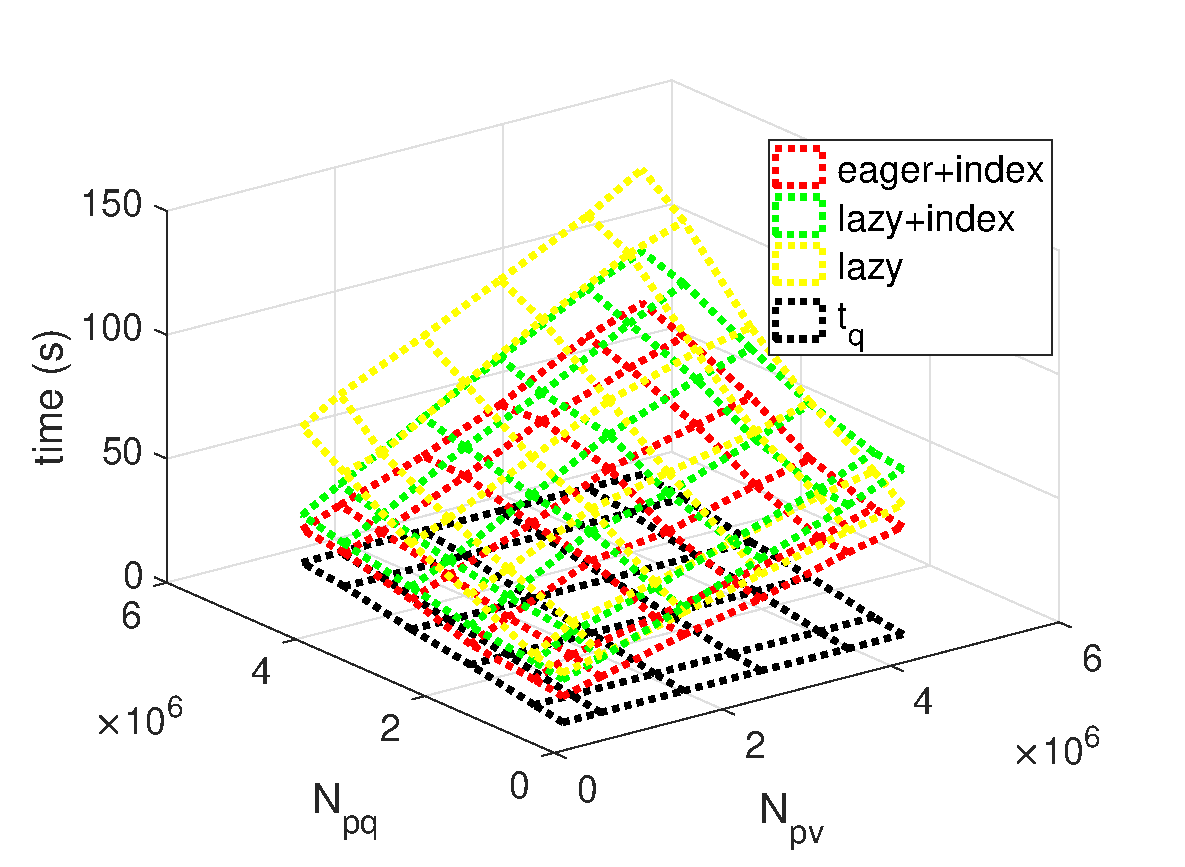
\includegraphics[height = 0.8\textwidth, width=1.2\textwidth]{Figures/synthetic_instance_size.eps}}
        \caption{$t_{cs}$ with varied $N_{pq}$ and $N_{pv}$}     \label{fig:stress_test_instance_size}
    \end{subfigure}
    \hfill
    \begin{subfigure}{0.30\textwidth}
    \hspace*{-0.8cm}
        \raisebox{-\height}{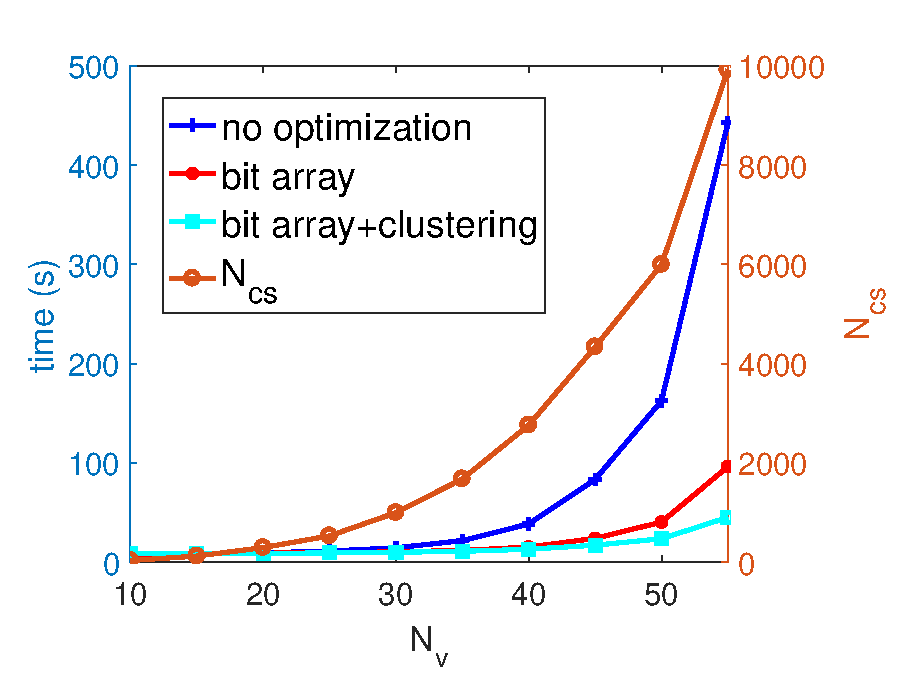
\includegraphics[height = 0.8\textwidth, width=1.2\textwidth]{Figures/synthetic_view_num.eps}}
        \caption{$t_{cs}$ with varied $N_v$}
        \label{fig:stress_test_view_num}
    \end{subfigure}
    \hfill
    \begin{subfigure}{0.30\textwidth}
    \hspace*{-0.8cm}
        \raisebox{-\height}{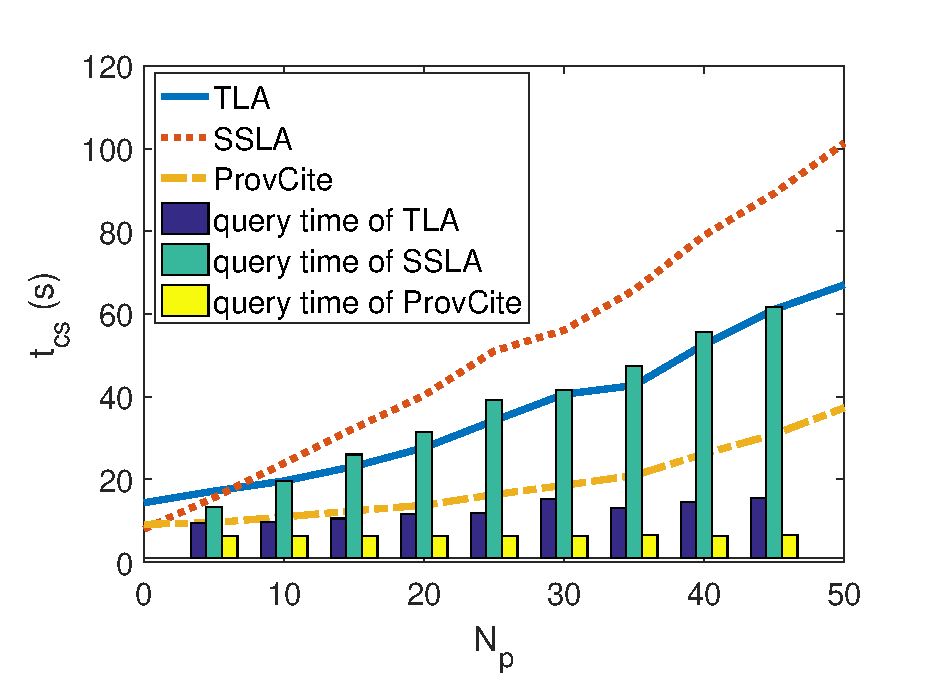
\includegraphics[height = 0.8\textwidth, width=1.2\textwidth]{Figures/synthetic_predicate_num.eps}}
        \caption{$t_{cs}$ with varied $N_p$}
        \label{fig:stress_test_predicate_num_time}
    \end{subfigure}
    \caption{Experimental results for synthetic workloads}
\end{figure*}

Table \ref{Table: notation_summary} provides a summary of the notation defined in this subsection.% which will be used in the remainder of this section.

\subsection{Experimental results}
We now report on results from the synthetic and realistic workloads.

\subsubsection{Synthetic workloads} 
We measured the impact of the size of provenance in both the query and view instances on time performance (Exp1), and the relative performance of \provalg\ and two implementations of the \rba, i.e. TLA and SSLA while varying the number of view mappings (Exp2) and number of view predicates (Exp3).

\textbf{Exp1.}  This experiment measures how the total reasoning time $t_{cs}$ is influenced by the total number of how-provenance monomials in the query instance ($N_{pq}$) as well as 
%the total number of how-provenance monomials 
in the view instance ($N_{pv}$). We randomly generate an aggregate query, and vary $N_{pq}$ by adding appropriate predicates. A fixed number of aggregate views are also generated such that there is exact one view mapping from each of them to the query and the total number of view mappings is fixed at 10, which is a reasonable number in practice. Both $N_{pq}$ and $N_{pv}$ are varied from 50K to 1M. $t_{cs}$ is measured for different ($N_{pq}$, $N_{pv}$) pairs under both the {\em eager} and {\em lazy} strategy.  

\textbf{Results.} 
The time performance, $t_{cs}$, is shown using 3D surfaces in Figure \ref{fig:stress_test_instance_size}, with the eager strategy shown in blue and the lazy strategy shown in red. It shows that the time performance under the eager strategy is only slightly better  than under the lazy strategy (10\% - 40\% faster). In the worst case, in which both $N_{pv}$ and $N_{pq}$ are 1 million, it takes no more than 150 seconds. This case will be rare, so the performance in practice should be much better. We also measured the extra space needed for the eager strategy, where the provenance of views is precomputed and stored in the database; it takes about 180 MB in the database to store the provenance for each view when the instance of the view includes up to 1 million how-provenance monomials. 

\textbf{Exp2.} The goal of this experiment is to compare the relative performance of \provalg, TLA and SSLA while varying the number of view mappings ($N_v$).
\eat{We call the system \provalg\ in the title, it is inconsistent to call it Prov here. I guess system is called \provalg\ while the algorithm is called Prov??}Since TLA and SSLA cannot handle aggregate views, only conjunctive views are used. So there is no difference between {\em eager} and {\em lazy} strategy since the provenance of views is not necessary. The query is a fixed aggregate query, with 500k how-provenance monomials in its instance. $N_v$ is varied from 1 to 50 and there are no predicates or lambda variables for each individual view. 

\textbf{Results.}
The experimental results are presented in Figure \ref{fig:stress_test_view_num}, which shows that $t_{cs}$ grows rapidly with the increasing number of view mappings ($N_v$) for all the three approaches. This is due to the fact that an exponential  number of covering sets are generated, which is inevitable. It is worth noting that \provalg\ \textit{outperforms} TLA when $N_v < 40$, and is on par with SSLA until $N_v >30$.
Furthermore it only adds a little extra overhead when $N_v > 40$ compared to the competitors. 


\textbf{Exp3.} In this experiment, \provalg\ is compared with TLA and SSLA while varying the total number of predicates ($N_p$) in views. Similar to Exp2, the query is an aggregate query which can generate about 500k tuples. The number of view mappings is fixed at 10 and there are initially no predicates. At each run, one more local predicate is added. As shown in \cite{wu2018data}, increasing $N_p$ can significantly influence the performance of TLA and SSLA by 1) increasing the query time since the query is extended to explicitly evaluate the satisfiability of predicates of the views in the query instance; 2) increasing the number of {\em reasoning groups} since we need to compute covering sets for each group and thus more {\em reasoning groups} in the query instance means more reasoning time. In theory, \provalg\ will also suffer from a large number of groups but will save on query time.

\textbf{Results.} The experimental results are shown in Figure \ref{fig:stress_test_predicate_num_time}, which matches the analysis above. As the number of predicates increases, $t_{cs}$ 
increases slowly for \provalg. In contrast, TLA and SSLA are twice as slow as \provalg\ for large $N_p$. To understand the reason for this, the query time for TLA and SSLA is also presented in this figure, which implies that the increasing query time becomes the major overhead for both TLA and SSLA, thus slowing down the computation.

{\bf Discussion.} The experiments reveal that all four metrics, $N_{pq}$ (the total number of how-provenance monomials in the query instance), $N_{pv}$ (the total number of how-provenance monomials in the view instance on average), $N_v$ (the total number of view mappings), $N_p$ (the total number of predicates under the view mappings) can affect the total reasoning time $t_{cs}$. In extreme cases, where the value of the metric is very large, bad performance is unavoidable.  However these cases are unlikely to happen in practice. We therefore expect reasonable time performance for realistic workloads. 

In the case of aggregate views where how-provenance is necessary, the  eager strategy beats the lazy strategy in terms of time.  The speedup is small (10\%-40\%), however, extra space is needed (up to 180 MB per view). So in practice, the choice between the eager or lazy strategy depends on whether speed or space is more important. In comparison to the previous approaches, TLA and SSLA, \provalg\ is not only more powerful in that it supports aggregate views but is also (surprisingly) frequently more efficient.  

\subsubsection{Realistic workloads}
\label{ssec: realistic}
The experimental results for realistic workloads are presented in Table \ref{Table: realistic_performance}, which includes the time to generate covering sets ($t_{cs}$) for both the lazy and eager strategies, as well as the metrics that can potentially affect the performance: the total number of how-provenance monomials in the query instance ($N_{pq}$), the total number of view mappings ($N_v$), the total number of predicates in the views under all the view mappings ($N_p$) and the query time to simply generate instance. Except for $q1$, most of $t_{cs}$ is less than 10 seconds for all queries. Although $N_{pq}$ is more than one million in $q1$, the total reasoning time ($t_{cs}$) is only about a half minute under both strategies, which is an acceptable considering the large query instance. To see how this compares to simply generating the query output, we list the query running time in the last column. When users are browsing the query result, the system can generate covering sets for all query tuples in the back-end, ready to instantly construct formatted citations when users select tuples of interest.

\eat{Comparing to time to simply generate query instance (See last column), $t_{cs}$ is still reasonable considering the large instance. When users are browsing the query result, the system can generate covering sets for all query tuple in the back-end, ready to construct formatted citations when users select tuples of interest.}

{\bf Discussion.} The experimental results above show that reasonable time performance can be guaranteed in practice where none of the crucial metrics become too large.  Revisiting the experimental results for synthetic workloads, when the total number of how-provenance monomials in the query instance ($N_{pq}$) is more than 1 million (as in $q1$), the reasoning time ($t_{cs}$) can be large (up to 150 seconds). However, the time shown for $q1$ is significantly smaller since the number of view mappings ($N_v$) is only 1, and the reasoning time relies on both $N_v$ and $N_{pq}$.




\begin{table}
\centering
\caption{Experimental results on realistic datasets}
\small
\begin{tabular}[!h]{|>{\centering\arraybackslash}p{0.8cm}|>{\centering\arraybackslash}p{1cm}|>{\centering\arraybackslash}p{1cm}|>{\centering\arraybackslash}p{1cm}|>{\centering\arraybackslash}p{0.25cm}|>{\centering\arraybackslash}p{0.25cm}|>{\centering\arraybackslash}p{1.5cm}|} \hline
Query& $t_{cs}$ (s) (eager) & $t_{cs}$ (s) (lazy)& $N_{pq}$&$N_v$&$N_p$&query time (s) \\ \hline
$q1$&22.51s&36.84s&1237914&1&0&1.02 \\ \hline
$q2$&4.40s&6.03s&203835&2&0&0.13 \\ \hline
$q3$&8.47s&11.23s&507515&2&0&1.15 \\ \hline
$q4$&3.72s&5.68s&416716&1&0&0.67\\ \hline
$q5$&4.56s&6.82s&243901&3&0&0.51 \\ \hline
\end{tabular}
\label{Table: realistic_performance}
\end{table} 



\section{Conclusions}\label{sec: conclusion}
We build on the connection to {\em data provenance} to develop a model for  data citation which is able to handle aggregate queries and views. The model reasons about citations at the level of tuples in the query result using provenance to enable citations to arbitrary subsets of the query result (fine-grained citation).  The \pbafull\ was implemented in \provalg, and extensive experiments conducted under both {\em synthetic} and {\em realistic workloads}.  The results show that \provalg\ can not only handle a larger class of queries than the Rewriting-Based Model~\cite{wu2018data} which assumes conjunctive queries and views, but is much faster in some cases.   The approach assumes a \textit{provenance-enabled DBMS}, and trade-offs between an {\em eager} versus {\em lazy} strategy for generating view provenance was explored. 

In future work, we would like to explore how to insert data citation into the larger citation ecosystem involving bibliometrics. We would also like to explore how to combine data citation with black-box computations, including Machine Learning models. 

\eat{
This is the first paper to build a {\em \pbafull} to connect the notion of {\em data citation} and {\em data provenance}, which is able to handle a larger class of queries and views i.e. aggregate queries and views compared to previous work and generate citations for query result at \textit{various granularity}. Efficient implementations for provenance reasoning, \provalg, are challenging but achieved by utilizing various optimization strategies. In \provalg, two different strategies are designed to deal with the provenance of views, which is either precomputed ({\em eager strategy}) or computed on the fly ({\em lazy strategy}). 

Extensive experiments are conducted under both {\em synthetic workloads} and {\em realistic workloads}. The experimental results justify the feasibility of \provalg\ to this model, which is not only powerful but also much faster in some cases compared to the implementations of \rba. Besides, the trade-offs between {\em eager strategy} and {\em lazy strategy} has been explored. The choice depends on users' preferences for speed or less space in practice.

In future work, we would like to explore how to integrate data citation into a larger citation ecosystem, which aims at efficiently and accurately computing and monitoring contributors' bibliometrics. Plus, considering the fact that machine learning algorithms are widely used and cited in {\em data science environment} and machine learning model is a special aggregate function, it will be also an interesting extension to automate citation generation process for machine learning pipeline.}
% \section{Optimizations in detail}
\subsection{Optimization on determining valid view mappings}
\subsubsection{Building indexes for query provenance}

Recall that the validity of view mapping $M$ for each query tuple $t_q$ depends on the mapping from a (or multiple) how-provenance monomial(s) of the view tuples to those of query tuple $t_q$. A naive solution is simply to scan the entire query provenance (at least once) for {\em every view mapping} to attempt to map every view provenance to the query provenance, which is expensive especially when $N_{pv}$ and $N_{pq}$ are large. Hashmap (mapping from the grouping attribute values to the how-provenance monomials in the query) seems to be helpful to speed up the searching, which, however, still needs to scan the entire query provenance for every view mapping. This issue is presented as below.

\begin{example}
Consider the following query:
\begin{tabbing}
$Q(G, COUNT(T), MAX(L), COUNT(E)):-Exon(E, L, T')$\\
\tab\tab$,Transcript(T, N, Ty, G), T = T', E <= 6$
% \tab\tab\tab$$
\end{tabbing}

Its instance along with the how-provenance polynomials are presented in Table \ref{Instance of Q}. By referencing the views defined in \ref{}, $V4-V6$ can potentially provide view mappings for $Q$. So their instance and how-provenance expressions are shown in Table \ref{Instance of V4'} to Table \ref{Instance of V6'}.

\begin{table}[htp]
\centering
\small
\caption{$Q(D)$ with how-provenance polynomials}\label{Instance of Q}
\begin{tabular}[t]{c|c|c|c|c||b|} \hhline{~-----}
&G&COUNT(T)&MAX(L)&COUNT(E)&prov\\ \hhline{~-----}
$t_{q1}$&1&1&1&1&$e_1*r_1$\\ \hhline{~-----}
$t_{q2}$&2&2&3&2&$e_2*r_2 + e_3*r_2$\\ \hhline{~-----}
$t_{q3}$&3&3&3&3&$e_4*r_3 + e_5*r_4 + e_6*r_4$\\ \hhline{~-----}
\end{tabular}
\bigskip
\caption{$V_4(D)$ with how-provenance polynomials}\label{Instance of V4'}
\begin{tabular}[t]{c|c|c||b|} \hhline{~---}
&G1&COUNT(T1)&prov\\ \hhline{~---}
$t_{v_41}$&1&1&$e_1*r_1$\\ \hhline{~---}
$t_{v_42}$&3&3&$e_4*r_3 + e_6*r_4 + e_7*r_4$\\ \hhline{~---}
\end{tabular}
\bigskip
\caption{$V_5(D)$ with how-provenance polynomials}\label{Instance of V5'}
\begin{tabular}[t]{c|c|c|c||b|} \hhline{~----}
&G1&MAX(L)&COUNT(E)&prov\\ \hhline{~----}
$t_{v_51}$&1&1&1&$e_1*r_1$\\ \hhline{~----}
$t_{v_52}$&2&3&2&$e_2*r_2 + e_3*r_2$\\ \hhline{~----}
$t_{v_53}$&3&3&4&$e_4*r_3 + e_5*r_4 + e_6*r_4 + e_7*r_4$\\ \hhline{~----}
\end{tabular}
\bigskip
\caption{Instance of relation $V6(D)$ with provenance}\label{Instance of V6'}
\begin{tabular}[t]{c|c|c||b|} \hhline{~---}
&G&COUNT(T)&prov\\ \hhline{~---}
$t_{v_61}$&1&1&$r_1$\\ \hhline{~---}
$t_{v_62}$&2&1&$r_2$\\ \hhline{~---}
$t_{v_63}$&3&2&$r_3 + r_4$\\ \hhline{~---}
\end{tabular}


\end{table}

There is an obvious view mapping from each view $V4-V6$ to $Q$, denoted as $M4-M6$, which should satisfy the {\em schema-level conditions} by comparing the grouping variables and aggregate variables between the views and the query. Then the {\em tuple-level conditions} are checked by comparing the how-provenance of each view tuple and that of each query tuples, As claimed earlier, a hashmap $HM$ is built to store the provenance information, in which the key-value pair stores the grouping attribute value and the set of how-provenance monomials respectively for each query tuple. For example, for query tuple $t_{q2}$ in the query $Q$, the entry in $HM$ corresponding to this tuple will be $\{2\rightarrow \{e_2*r_2, e_3*r_2\}\}$ (denoted by $En$) where $2$ is the value for grouping attribute $G$ while $\{e_2*r_2, e_3*r_2\}$ is the how-provenance monomial set for $t_{q2}$. For a view tuple (e.g. $t_{v_52}$), in order to build the potential monomail mappings for its how-provenance monomial, we firstly retrieve the {\em candidate entry} (e.g. $En$ for $t_{v_52}$) from $HM$ with the value of the grouping attributes (that are mapped to the grouping attributes under the view mapping). Then for every monomial of this view tuple (e.g. $e_2*r_2$), we can check its existence in the candidate entry (with $O(1)$ time for every monomial) and thus determine whether the provenance monomial mappings satisfy the validity conditions

However, it is worth noting that $HM$ is not helpful for determining the validity of $M6$ since the how-provenance monomials in $V6(D)$ only include one provenance token (e.g. see tuple $t_{v_62}$, it includes on provenance monomial $r_2$), for which we cannot determine their existence in some entry in $HW$ in $O(1)$ time. For example, the {\em candidate entry} for $t_{v_62}$ is still $En$, but $r_2$ is not the same as either of the two monomials in the monomial set ($e_2*r_2$ and $e_3*r_2$), which, however can be mapped to either $e_2*r_2$ or $e_3*r_2$ under view mapping $M6$ according to the validity conditions. So we either need to consume more time for search in $HW$ or have to reconstruct another hashmap $HW'$ which simply includes the portion of how-provenance monomials involved in $M6$ (such that the search takes only $O(1)$), either of which case can result in another full scan of the entire query provenance.

In order to avoid multiple scans over query provenance, we built an index $I$ for each single provenance token to indicate which query tuples (represented by grouping attribute values) and which provenance monomials it lies in. For example, for token $r_4$ in the query provenance, since it is in the second and third monomial in the query tuple $t_{q3}$, such {\em coordinate information} is thus stored in the index $I$ taking $r_4$ as the key. For a how-provenance monomial in the view, e.g. $e_4*r_3$ in $t_{v_42}$, to determine whether it can be mapped to some query provenance monomial, we can retrieve the {\em coordinate information} for $e_4$ and $r_3$ respectively (if any) and then perform intersection over the {\em coordinate information} of the two tokens to check whether they coexist in some how-provenance monomial in the query provenance. For instance, after taking the intersection operations, the common position for $e_4$ and $r_3$ is the first monomial in the tuple $t_{q3}$. We can further optimize the intersection operations by representing the monomial coordinate with bit array and applying bit AND operations for speed-ups. It turns out that this strategy only requires full scan over the query provenance for all the view mappings.

\subsubsection{Parallelly determine valid view mappings}
We also observe that the validity of one view mapping is independent from others, which thus drives us to parallelize the computation. One straightforward way is to create one thread for each view mapping, which, however can degrade the performance due to the overhead to retrieve the view provenance from the database and the memory consumption in each thread. After trial and errors, we find that batch processing 5 view mappings each time can lead to best performance. Note that the system is built on single machine, it is worth trying to migrate it to distributed systems for further performance gains in the future.

\subsubsection{Materializing the view content along with provenance}


\subsection{Optimization on computing covering sets}
As we observed in \cite{wu2018data}, it is a time-consuming step to compute {\em all} covering sets after the validity of view mappings are determined. Compared to \cite{wu2018data}, two strategies are applied to speed up the covering sets calculation, i.e. 1) representing coverings sets using bit arrays; 2) applying clustering algorithms to avoid an explosion of intermediate results. 

\subsubsection{Introducing bit arrays}
The computation of covering sets involves merging valid view mappings by each covered aggregate term incrementally and removing duplicates. For example, for $Q$, the aggregate term $COUNT(T)$, $MAX(L)$ and $COUNT(E)$ are covered by $\{M_3, M_4, M_6\}$ (denoted by $S_1$), $\{M_5, M_6\}$ (denoted by $S_2$) and $\{M_3, M_4\}$ (denoted by $S_3$) respectively. To compute covering sets, the cross product of $S_1$ and $S_2$ are computed first, which leads to some view mapping combinations (called {\em sub-covering sets thereafter}) that can cover both the aggregate terms. For instance, $\{M_3, M_5\}$ is one such sub-covering set. The construction of sub-covering sets (and covering sets ultimately) involves merging the view mappings and the aggregate terms and relational subgoals covered by them, which facilitate the following redundancy removal step. For example, $\{M_3,M_6\}$ (picked from $S_1$ and $S_2$ respectively) can jointly cover both the aggregate terms and relational subgoals of $Q$, which, however, is redundant with respect to $\{M_6\}$ (picked from $S_1$ and $S_2$ and one copy is retained) since $\{M_6\}$ is a {\em subset} of $\{M_3,M_6\}$ but still covers the same aggregate terms and relational subgoals as $\{M_3,M_6\}$. So it is safe to remove $\{M_3, M_6\}$ at this point. Then the resulting sub-covering sets are combined with the view mapping set in $S_3$ to compute the final covering sets.

Note that two key operations are essential in this step, i.e. 1) merging view mappings and the terms covered by them; 2) removing redundancy by subset checking, which can be optimized by applying bit operations. For example, we can encode the view mapping $M_3-M_6$ as $\{0,1,2,3\}$, the aggregate terms ($COUNT(T)$ and $MAX(L)$) as $\{0, 1\}$ and the relational subgoals ($Exon$ and $Transcript$) as $\{0, 1\}$. Three bit arrays are introduced for view mapping combinations, aggregate terms and relational subgoals, in which $i_th$ bit is 0 or 1 if $i_th$ view mapping/aggregate term/relational subgoal is included or missing in the sub-covering set. For example, for sub-covering set $\{M_3, M_6\}$, we use bit array 1001 to represent the view mapping in it (the leftmost 1 is in the 0th bit, which indicates the existence of $M_3$). Similarly, since they cover both the aggregate terms and relational subgoals, the other two bit arrays will be both 11. So when merging sub-covering set (or view mappings) with other sub-covering set (or view mappings), we can apply bit OR operations over the three bit arrays. Similarly, for subset checking operation, bit AND operation is applicable.



\subsubsection{Applying clustering algorithms}
The order of merging view mapping sets (e.g. merging $S_1$, $S_2$ first or $S_1$, $S_3$ first) have no effect on the final result but can bring about significant performance differences. For example, if $S_1$ and $S_3$ are merged first, after removing duplicates, the intermediate result will be $\{\{M_3\}, \{M_4\}\}$, which is smaller than the result of the other option (merging $S_1$ and $S_2$ first), i.e. $\{\{M_3, M_5\}, \{M_4, M_5\}, \{M_6\}\}$. For the purpose of better merging strategy, clustering algorithms are applied such that the view mapping sets that are similar to each other can be clustered and thus merged first (e.g. $S_1$ and $S_3$). In ProCite, affinity propagation clustering algorithm \cite{dueck2007non} is used since it does not require pre-defined cluster number.




\eat{; and 3) query tuples associated with the same set of valid view mappings form a {\em reasoning group} to avoid repetitive computations of covering sets. For example, $t_{q1}$ and $t_{q2}$ have the same set of valid view mappings, $\{M_5\}$, which should end up with the same covering sets. So those two tuples are grouped together to compute covering sets once. These optimizations can result in orders of magnitude speed-up.} %However, due to the space limit, the details are not provided here. 



\end{example}
% \begin{appendix}
You can use an appendix for optional proofs or details of your evaluation which are not absolutely necessary to the core understanding of your paper. 

\section{Details of approaches}

In this section, the details of provenance approach is presented step by step and the corresponding pseudo-code is provided. One key step is to derive the valid view mappings, which depends on checking the satisfiability of {\em schema-level approach} and {\em tuple-level approach} for each candidate view mapping. So we present the details of 
determining view mappings satisfying {\em schema-level approach} in Algorithm \ref{view_mapping_schema_level} and the details of continuing filtering out view mappings violating {\em tuple-level approach} for each individual query tuple in Algorithm \ref{view_mapping_tuple_level}.

\begin{algorithm}[h!] 
\footnotesize
 \SetKwInOut{Input}{Input}
 \SetKwInOut{Output}{Output}
 \Input{a set of views: $\mathcal{V} = \{V_1, V_2,...,V_k\}$, user query: $Q$, a Database instance $D$}

 \Output{the set of all covering sets for each tuple in $Q(D)$}

{\em Preprocessing step}: Return a set of view mappings $\mathcal{M}$ and the provenance of $Q$ and each $V$

{\em Reasoning valid view mapping step}: For each query tuple $t$, determine valid view mappings by comparing the provenance of  $Q$ and the provenance of $V$

{\em Covering sets calculation step}: Calculate covering sets based on derived valid view mappings for each query tuple, which will be the output of the algorithm.
%  }
%  \For{each view mapping $M \in \mathcal{M}$}{
 
%     Derive lambda terms $L(M)$ and the predicates $condition(M)$ under $M$
    
%     Add all lambda terms in $L(M)$ to $\bar{X}'$
    
%     Add boolean expressions of all the global conditions in $condition(M)$ to $\bar{X}''$
%  } 
%  \For{each relation $B_i$ in the body of $Q$}
%  {
%     Add the view vectors $Vec(B_i)$ to $\bar{X}'$.
%  }

%  Construct the extended query $Q_{ext1}$ with the following form:

%  $Q_{ext1}(\bar{X}') :- B_1(\bar{X_1}), B_2(\bar{X_2}), \dots, B_m(\bar{X_m}), condition(Q)$

 \Return $\mathcal{M}$

 \caption{Derive all possible view mappings in the schema level}
 \label{view_mapping_schema_level}
 \end{algorithm}


\begin{algorithm}[h!] 
\footnotesize
 \SetKwInOut{Input}{Input}
 \SetKwInOut{Output}{Output}
 \Input{a set of views: $\mathcal{V} = \{V_1, V_2,...,V_k\}$, user query:
 $Q(\bar{X}, Agg_1(\bar{X'_{1}}), \dots, Agg_s(\bar{X'_{s}})) :- B_1, B_2, \dots, B_m, condition(Q)$, a set of possible view mappings $\mathcal{M}$, a query tuple $t \in Q(D)$}

 \Output{the set of valid view mapping $\mathcal{M}_t$}

 Initialize $\mathcal{M}_t = \{\}$
 
 Suppose the assignment to tuple $t$ is $\Gamma$ and the isomorphism between each subgoal and how-provenance under the assignment $\Gamma$ is $F$.

Suppose the how-provenance polynomial of $t$ is $W = \sum_{i=1}^rW_i$

% Create a multiset $\bar{W}$ to store all the monomials in $W$


 \For{each view mapping $M \in \mathcal{M}$ which maps view $V$ to $Q$}
 {

	\For{each how-provenance monomial $W_i$}
 	{
    	\For{each how-provenance token $w_{ij}$ in $W_i$}
        {
        	Subgoal $R=F^{-1}(w_{ij}|\Gamma)$
            
            \If{a subgoal $R'$ in the body of $V$ can be mapped to $R$ under $M$}
            {
      			Assign the base relation tuple $t'$ which is associated with how-provenance token $w_{ij}$ to $R'$      		
            }
        }
        \If{any predicate of $V$ is evaluated to be false}
        {
        	\textbf{break}
        }
    }
    \eIf{$V$ is a conjunctive view}
    {
		add $M$ to $\mathcal{M}_t$
    }
    {

		Initialize potential valid view tuple sets $\mathcal{T}_v$
    	
        Suppose grouping variable set $\bar{Y}$ in the head of $V$ is mapped to $\bar{X}$, i.e. $\phi(\bar{Y}) = \bar{X}$
        
        Initialize $W' = 0$
        
        
		\For{every view tuple $t_v \in V(D)$}
        {
        
        	Suppose that the corresponding value assignment in $t_v$ is $\Gamma'$
            
			\If{$\Gamma'(\bar{Y}) = \Gamma(\bar{X})$ }
            {
            	\tcc{$t_v$ has the same values on attributes $\bar{Y}$ as $t$ has on attributes $\bar{X}$}
                
                Suppose the how-provenance polynomial of $t_v$ is $W'$
                
                \If{every monomial in $W'$ can be mapped to some monomial in $\bar{W}$}
                {
                	$W := W + W'$
                }
            }
        }
        
        \If{W == W'}
        {
        	add $M$ to $\mathcal{M}_t$
        }
        
%         \While{$\bar{W}$ shrinks}
%         {
% 			\For{every view tuple $t_v \in \mathcal{T}_v$}
%             {
% 				\If{every monomial in $W'$ can be mapped to some monomial in $\bar{W}$}
%                 {
%                 	Remove the monomials in $W'$ from $\bar{W}$
%                 }
%             }        
%         }
        
%         \If{$\bar{W}$ is empty}
%         {
%         	Add $M$ to $M_t$
%         }
    }
 }
 \Return $\mathcal{M}$
 \caption{Derive valid view mappings for each tuple}
 \label{view_mapping_tuple_level}
 \end{algorithm}


Please use readable font sizes in the figures and graphs. Avoid tempering with the correct border values, and the spacing (and format) of both text and captions of the PVLDB format (e.g. captions are bold).

At the end, please check for an overall pleasant layout, e.g. by ensuring a readable and logical positioning of any floating figures and tables. Please also check for any line overflows, which are only allowed in extraordinary circumstances (such as wide formulas or URLs where a line wrap would be counterintuitive).

Use the \texttt{balance} package together with a \texttt{\char'134 balance} command at the end of your document to ensure that the last page has balanced (i.e. same length) columns.

\end{appendix}
%ACKNOWLEDGMENTS are optional
\section{Acknowledgments}
This research was partially funded by NSF IIS 1302212 and NSF ACI 154736. The authors thank Peter Buneman for conceiving the idea that data citation is a computational challenge and recognizing its connection to provenance, and to Val Tannen for discussions on query rewriting and provenance.
%; and Boris Glavic for his support in understanding details of GProM's source code.


% The following two commands are all you need in the
% initial runs of your .tex file to
% produce the bibliography for the citations in your paper.
\newpage
\bibliographystyle{abbrv}
\bibliography{vldb_sample}  % vldb_sample.bib is the name of the Bibliography in this case
% You must have a proper ".bib" file
%  and remember to run:
% latex bibtex latex latex
% to resolve all references

% \subsection{References}
% Generated by bibtex from your ~.bib file.  Run latex,
% then bibtex, then latex twice (to resolve references).

%APPENDIX is optional.
% ****************** APPENDIX **************************************
% Example of an appendix; typically would start on a new page
%pagebreak



\end{document}
